\documentclass[preprint,12pt]{elsarticle}

\usepackage{graphicx}
\usepackage{amssymb}
\usepackage{amsmath}
\usepackage{hyperref}
\usepackage{booktabs}
\usepackage{color}
\usepackage{algorithm}
\usepackage{algorithmic}
\usepackage{bm}
\usepackage{natbib}

% Layout robustness: absorb long inline-math lines and break long URLs
\setlength{\emergencystretch}{3em}
\makeatletter
\g@addto@macro\UrlBreaks{\do\a\do\b\do\c\do\d\do\e\do\f\do\g\do\h\do\i\do\j\do\k\do\l\do\m\do\n\do\o\do\p\do\q\do\r\do\s\do\t\do\u\do\v\do\w\do\x\do\y\do\z\do\A\do\B\do\C\do\D\do\E\do\F\do\G\do\H\do\I\do\J\do\K\do\L\do\M\do\N\do\O\do\P\do\Q\do\R\do\S\do\T\do\U\do\V\do\W\do\X\do\Y\do\Z}
\makeatother

\journal{Journal of Sound and Vibration}

\begin{document}

\begin{frontmatter}

\title{Multiplication-Free Stochastic Semi-Discretization for the Efficient Moment Stability Analysis of Vibration Systems with Delay}

\author[1]{D\'aniel Bachrathy\corref{cor1}}
\ead{bachrathy@mm.bme.hu}
\author[1]{Henrik T. Sykora}

\address[1]{Department of Applied Mechanics, Faculty of Mechanical Engineering, Budapest University of Technology and Economics, M\H{u}egyetem rkp. 3., H-1111 Budapest, Hungary}

\cortext[cor1]{Corresponding author}

\begin{abstract}
The moment-stability analysis of stochastic time-delayed vibration systems by the Stochastic Semi-Discretization Method (SSDM) is limited by the $\mathcal{O}(p^4)$ cost of assembling and multiplying the second-moment step operators over one period. This work introduces the Multiplication-Free Stochastic Semi-Discretization Method (MF-SSDM), which evaluates the action of the identical period operator by an in-place block recursion at strictly quadratic $\mathcal{O}(p^2)$ cost; the measured advantage over the explicit period product reaches $1.3\times10^4$ in time and $1.8\times10^4$ in solver memory allocation at resolutions as low as $p=192$. Four further contributions extend the practical reach of the framework. A Kronecker-factored formulation of the It\^o-contraction operator replaces the $\mathcal{O}(d^4)$ pre-contracted tensors by $\mathcal{O}(K d^2)$ sampled factors --- algebraically identical to the dense form --- extending the analysis to hundreds of state variables (a 100-DOF oscillator chain and a finite-element beam with a $2.16$-million-unknown covariance problem are demonstrated). A Gauss--Legendre collocation reformulation of the covariance blocks lifts the measured second-moment convergence order from one (observed for the classical scheme at any deterministic interpolation order) to $2S$ in the stage number $S$, with rates consistent with order eight at $S=4$; owing to its $(2S+2)^2$ covariance scaling this high-order route targets low- and moderate-dimensional systems, complementary to the factored operator that covers the high-dimensional regime at classical order. A fractional-limit generalization of the integrated-history blocks extends the high-order route to smoothly time-varying delays --- spindle-speed variation being the motivating case --- with measured orders of $3.5$ ($S{=}2$) and $5.9$ ($S{=}3$) on an SSV turning model, at or near $2S$ and above the guaranteed $S{+}1$ floor. Finally, a structural order limitation caused by delayed reads of noise-driven (Brownian-rough) state components --- the delayed derivative term of a PD controller being the archetype --- is identified and removed by integrated-history reads complemented by an exact integration-by-parts reformulation. The framework is demonstrated on a spindle-speed-variation milling model with time-varying delay, where the variance-based surface-quality boundary is shown to lie strictly below the stability boundary.
\end{abstract}

\begin{highlights}
\item Multiplication-free stochastic semi-discretization for delayed vibration systems
\item Second-moment cost reduced from $\mathcal{O}(p^4)$ to $\mathcal{O}(p^2)$ in time and memory
\item Kronecker-factored It\^o operator reaches hundreds of state variables
\item Collocation covariance blocks raise the measured moment order to $2S$
\item Fractional-limit history blocks extend the high order to time-varying delays
\item Integration by parts restores high order for delayed PD feedback
\end{highlights}

\begin{keyword}
Time-delay systems \sep Stochastic stability \sep Semi-discretization \sep Multiplication-free algorithm \sep Machine tool chatter \sep Moment stability
\end{keyword}

\end{frontmatter}

\section*{Nomenclature}
\begin{tabbing}
  $d$, $m$ \quad\quad \= State dimension; number of independent Wiener processes \\
  $\mathbf{x}(t)$ \> State vector in $\mathbb{R}^d$; $W_k(t)$: independent Wiener processes \\
  $\mathbf{A}(t), \mathbf{B}(t)$ \> Deterministic drift and delayed-coupling matrices \\
  $\boldsymbol{\alpha}_k(t), \boldsymbol{\beta}_k(t)$ \> Multiplicative noise coefficient matrices (present / delayed read) \\
  $\boldsymbol{\gamma}_k(t)$, $\mathbf{c}(t)$ \> Additive noise vector; deterministic excitation vector \\
  $\tau$, $T$ \> Time delay; principal period \\
  $\Delta t$, $p$, $r$ \> Time step; steps per period ($T = p\Delta t$); steps per delay ($\tau = r\Delta t$) \\
  $q$ \> Interpolation order of the classical semi-discretization \\
  $\mathbf{y}_n$ \> Augmented state history vector in $\mathbb{R}^{d(r+1)}$ \\
  $\mathbf{M}_n$ \> Second-moment matrix $\mathbb{E}[\mathbf{y}_n \mathbf{y}_n^\top]$ (= covariance for zero mean) \\
  $\mathbf{C}_{i,j}^{(n)}$ \> $d \times d$ block of $\mathbf{M}_n$; $D$: dimension of $\operatorname{vech}\mathbf{M}$ \\
  $\mathbf{F}_n, \mathbf{G}_{n,k}(s)$ \> Deterministic transition matrix; sampled stochastic coefficient \\
  $\mathcal{H}$, $\rho(\cdot)$ \> Second-moment period operator; spectral radius \\
  $\mathcal{S}$, $\mathcal{U}_n$ \> History shift operator; boundary-injection operator \\
  $K$, $\tilde{\mathbf{G}}^{(\kappa),w}_{n,k}$ \> It\^o-isometry quadrature count; weight-scaled samples (Kronecker factors) \\
  $S$, $\mathbf{Y}_i$, $\mathbf{J}_i$ \> Collocation stages; stage values; integrated-history DOFs \\
  $N$ \> Stored history sub-points per period ($N = p(2S+2)$ for GL-$S$) \\
  $k_P, k_D$ \> Delayed proportional / derivative feedback gains \\
  $Y_c$ \> Antiderivative of the rough state component $x_c$ (IBP) \\
  $\zeta$ \> Damping ratio \\
  $z$, $a_D$, $K_n/K_t$ \> Number of cutter teeth; radial immersion; cutting-force ratio \\
  $w$, $\Omega_0$ \> Dimensionless depth of cut; dimensionless mean spindle speed \\
  $\mathrm{RVA}$, $T_{\mathrm{SSV}}$ \> Relative amplitude and period of the spindle speed variation \\
  $\sigma_c$, $\sigma_a$, $\sigma_P$ \> Multiplicative (cutting-coefficient / axial-load) and additive noise intensities
\end{tabbing}

\section{Introduction}
\label{sec:intro}

The interaction between time delays and stochastic perturbations is a defining characteristic of many critical engineering systems \cite{Stepan1989, Tobias1965, Tlusty1954, Altintas2012}. In manufacturing, the regenerative chatter effect in milling and turning is classically governed by deterministic Delay Differential Equations (DDEs), where the time delay corresponds to the tooth-passing period of the cutter in milling, or the workpiece revolution period in turning \cite{Altintas2012, Insperger2011, Munoa2016, Quintana2011}. Real-world machining environments, however, are inherently noisy: stochastic variations of the cutting force, non-uniform tool wear, and random spindle speed fluctuations introduce persistent broadband noise that transforms these deterministic models into Stochastic Delay Differential Equations (SDDEs) \cite{Long2007, Fodor2020, Sykora2021_MSSP}.

Predicting the stability of such systems is significantly more complex than in the deterministic case. While deterministic stability is typically determined by the spectral radius of a monodromy matrix (Floquet theory), recent research has demonstrated that deterministic stability limits can rarely be approached in practice in real machining operations \cite{Sykora2021_MSSP}. As the system parameters approach the deterministic stability boundary, the damping of the dominant vibration modes diminishes, and even small random perturbations are amplified into large-amplitude sustained oscillations well before the theoretical limit is crossed \cite{Sykora2021_MSSP, Bachrathy2021_CIRP}. Consequently, a sharp ``onset of chatter'' cannot be identified in noisy environments.

Therefore, stochastic stability necessitates the investigation of moment dynamics rather than individual sample paths \cite{Arnold1973, Khasminskii2011, Mao2007}; classical approximate routes to stochastic vibration analysis include stochastic averaging \cite{Roberts1986}, while direct numerical treatment of SDDEs is covered by \cite{Kloeden1992, Higham2001, Buckwar2000}. In particular, second-moment stability provides a rigorous condition for the boundedness of the system's variance, ensuring that vibrations do not grow without limit in a mean-square sense. More importantly for practical engineering, the \emph{stationary} second moment is directly usable: the stationary variance of the tool vibration maps onto the surface location error and the macroscopic surface roughness of the machined workpiece \cite{HoneycuttSchmitz2017, Fodor2020, Fodor2024_PSD}, so a strict upper bound on the stationary variance ensures the required surface quality and establishes a pragmatic, safe operational window \cite{Sykora2020b, Fodor2024_PSD}.

The Semi-Discretization Method (SDM) has been a cornerstone for analyzing time-periodic delayed systems for decades \cite{Insperger2002, Insperger2011, Bachrathy2013}. Its extension to stochastic systems is the Stochastic Semi-Discretization Method (SSDM) \cite{Sykora2019, Sykora2020a, Sykora2020b, Fodor2023_PEM}. While SSDM preserves the robustness of the original scheme, the dimension of the second-moment mapping scales quadratically with the discretization resolution $p$. The recursive evaluation of this mapping results in a computational complexity of $\mathcal{O}(p^4)$ even with sparse optimizations \cite{Sykora2019}. This resolution bottleneck effectively prohibits high-resolution parameter studies and the analysis of multi-degree-of-freedom (multi-DOF) models.

A fundamentally different route has recently been opened by Iklodi and Dankowicz \cite{Iklodi2026}, who dispense with discretization altogether: for linear, \emph{time-invariant} SDDEs with a single constant delay they derive semi-analytic algebraic equality conditions for the second-moment stability boundary from an advection-type correlation boundary-value problem, trace them by parameter continuation at a cost that scales only with the square of the state dimension, and obtain a closed-form condition in the scalar case. Where it applies, this is the sharper instrument: it carries no discretization error and returns the exact boundary. Its scope is, however, complementary to the present work --- the underlying reduction presumes constant coefficients and a single constant point delay, so the time-periodic, time-varying-delay systems that motivate this paper (milling under spindle-speed variation, parametrically excited structures) lie outside it, as do multiple and distributed delays, which the authors leave to future work. We note further that the substantial speed-up reported there is measured against a \emph{direct} pseudo-spectral discretization --- that is, against precisely the $\mathcal{O}(p^4)$-type resolution bottleneck that the present paper removes; the reformulations developed below reduce that cost by orders of magnitude (Section \ref{sec:results}), so on the subclass where both apply the practical distance between discretization-free algebra and a well-implemented discretization is considerably smaller than that comparison suggests.

In this paper, we address this fundamental limitation by proposing the Multiplication-Free Stochastic Semi-Discretization Method (MF-SSDM). Building upon the multiplication-free evaluation of the deterministic semi-discretization mapping \cite{BachrathyMFSD}, we reformulate the stochastic covariance mapping. By treating the history evolution as a shift operator and computing only the localized block-sparse updates, we reduce the complexity to strictly quadratic $\mathcal{O}(p^2)$. We further integrate this approach with Krylov subspace solvers \cite{Saad1986, Haegeman2021}, allowing for stability and stationary solution calculations without ever constructing the large mapping matrices explicitly.

Beyond the complexity reduction in $p$, three further methodological contributions are presented, each following the same pattern: a concrete limitation of the previous state of the art, a structural remedy, and quantitative numerical evidence. First, for systems with many degrees of freedom, the classical assembly of the second-moment operator stores dense $d^2 \times d^2$ It\^o-contraction blocks whose $\mathcal{O}(d^4)$ footprint becomes the dominant obstacle well before the delay resolution does. We show that these blocks are Kronecker-structured sums, and derive a \emph{factored operator} formulation which applies the identical linear map through $\mathcal{O}(K d^2)$ storage and $\mathcal{O}(K d^3)$ work, where $K$ is the number of quadrature samples of the It\^o isometry. The factored form is algebraically identical to the dense one --- spectral radii and stationary moments agree to machine rounding --- while extending the tractable range from $d \approx 10$ to systems with hundreds of state variables. Second, we document a barrier that is easily overlooked: however high the interpolation order of the deterministic semi-discretization, the measured convergence of the \emph{second moment} remains first order, because the accuracy is limited by the per-step stochastic quadrature rather than by the deterministic interpolation. We lift this barrier by a Gauss--Legendre collocation reformulation of the covariance blocks, which carries stage values and integrated-history quantities per step and attains measured order $2S$ in the number of stages $S$ (rates consistent with order eight), so that a handful of steps per period can outperform the classical scheme extrapolated to $p = 10^4$. Third, we analyze how the \emph{structure} of the delayed coupling limits the attainable convergence order in the presence of multiplicative noise: whenever the delayed drift term reads a state component that is directly driven by the Wiener process (a ``rough'' component, e.g.\ a velocity in a mechanical system under delayed derivative feedback), sampling-based quadrature of the delayed term incurs an irreducible low-order error. The integrated-history states of the collocation blocks evaluate the delayed coupling exactly and remove the collapse for mechanical PD feedback; an integration-by-parts (IBP) reformulation of the delayed-coupling integral complements this by shifting rough reads onto smooth (integrated) components, further reducing the error constants.

The paper is structured as follows. Section \ref{sec:theory} establishes the explicit mapping from SDDE coefficients to the discrete-time mapping matrices and identifies the period operator --- a product of $p$ step operators --- as the classical bottleneck. Section \ref{sec:mf_algo} derives the multiplication-free block updates and details the implementation using virtual circular buffers. Section \ref{sec:kron} introduces the Kronecker-factored operator for high-dimensional systems. Section \ref{sec:colloc} presents the high-order collocation reformulation of the covariance blocks and its automatic structural pruning, together with its fractional-limit extension to smoothly time-varying delays. Section \ref{sec:ibp} analyzes the convergence-order limitation induced by rough delayed reads and presents the IBP treatment for delayed PD control. Section \ref{sec:results} provides an extensive numerical validation, including a work-precision study against the explicit period product, the PD-controlled stochastic Mathieu example with full work-precision comparisons of all schemes, and an SSV milling case study with a time-varying delay and a linear force model; the GPU implementation and a finite-element beam study are reported in the appendices. Section \ref{sec:conclusions} summarizes the results.

\section{Stochastic Semi-Discretization Framework}
\label{sec:theory}

In this section, we lay the mathematical foundation for the stochastic stability analysis and describe the classical SSDM implementation. We consider a linear system of SDDEs representing a multi-DOF mechanical system subjected to non-autonomous drift, delay, and both additive and multiplicative noise:
\begin{equation}
\label{eq:sdde_theory}
\begin{split}
\mathrm{d}\mathbf{x}(t) = {}& \left[\mathbf{A}(t)\mathbf{x}(t) + \mathbf{B}(t)\mathbf{x}(t-\tau) + \mathbf{c}(t)\right] \mathrm{d}t \\
&+ \sum_{k=1}^m \left[\boldsymbol{\alpha}_k(t)\mathbf{x}(t) + \boldsymbol{\beta}_k(t)\mathbf{x}(t-\tau) + \boldsymbol{\gamma}_k(t)\right] \mathrm{d}W_k(t),
\end{split}
\end{equation}
interpreted in the It\^o sense; all coefficient matrices are bounded, piecewise-continuous, and $T$-periodic, which guarantees a unique strong solution with finite second moments for square-integrable initial data \cite{Mao2007}. When a physical broadband excitation of non-zero correlation time is modeled, the Wong--Zakai limit yields the Stratonovich interpretation, and the corresponding drift correction $\tfrac12\sum_k \boldsymbol\alpha_k(\boldsymbol\alpha_k \mathbf{x} + \boldsymbol\beta_k \mathbf{x}_\tau + \boldsymbol\gamma_k)$ must be absorbed into $\mathbf{A}, \mathbf{B}, \mathbf{c}$ before applying the present (It\^o-based) framework.

\paragraph{Mean-square stability and the quantity computed.}
The zero solution of the homogeneous part of Eq.~\eqref{eq:sdde_theory} is called \emph{mean-square (second-moment) exponentially stable} if $\mathbb{E}\,\|\mathbf{x}(t)\|^2 \to 0$ exponentially for every square-integrable deterministic initial segment. The exact second-moment dynamics of an SDDE is infinite-dimensional --- it propagates the two-time covariance kernel $\mathbf{C}(\theta_1,\theta_2,t) = \mathbb{E}[\mathbf{x}(t+\theta_1)\mathbf{x}(t+\theta_2)^\top]$ on $[-\tau,0]^2$. The semi-discretization below replaces this kernel by its values on a finite grid, producing a finite-dimensional linear map $\mathcal{H}$ over one period; the discrete stability criterion is $\rho(\mathcal{H}) < 1$. The convergence of $\rho(\mathcal{H})$ to the exact second-moment Floquet radius as the resolution grows is inherited from the consistency of the underlying discretization \cite{Sykora2019,Sykora2020a} and is verified numerically to high accuracy throughout this paper (self-convergence plus an independent-solver certificate in Section \ref{sec:results_pd}); no formal convergence proof is claimed here. Unless stated otherwise the examples have zero-mean excitation ($\mathbf{c}\equiv\mathbf{0}$ and zero-mean initial data), so that $\mathbf{M}_n$ below is simultaneously the second moment and the covariance; the implementation propagates the mean jointly with the second moment in the general case, and the affine coupling terms are omitted from the displayed formulas for brevity.

\subsection{State-Augmented Mapping}
The semi-discretization procedure partitions the delay $\tau$ into $r$ intervals of length $\Delta t = \tau/r$ (in this and the next section the derivation is displayed for the common case $T = \tau$, i.e.\ $p = r$; the bookkeeping for $\tau \ne T$ only changes the buffer length). The continuous history is approximated by the augmented vector $\mathbf{y}_n = [\mathbf{x}_n^\top, \mathbf{x}_{n-1}^\top, \dots, \mathbf{x}_{n-r}^\top]^\top \in \mathbb{R}^{d(r+1)}$. Over a single time step $\Delta t$, the evolution is governed by:
\begin{equation}
\label{eq:discrete_map}
\mathbf{y}_{n+1} = \mathbf{F}_n \mathbf{y}_n + \sum_{k=1}^m \mathbf{G}_{n,k} \mathbf{y}_n \Delta W_{n,k} + \mathbf{q}_n.
\end{equation}

\subsection{Explicit Matrix Components and Stochastic Integration}
The transition matrices $\mathbf{F}_n$ and $\mathbf{G}_{n,k}$ share the following block-sparse structures:
\begin{equation}
\mathbf{F}_n = \begin{bmatrix} \mathbf{F}_{n,0} & \mathbf{0} & \dots & \mathbf{0} & \mathbf{F}_{n,r} \\ \mathbf{I} & \mathbf{0} & \dots & \mathbf{0} & \mathbf{0} \\ \vdots & \ddots & & \vdots & \vdots \\ \mathbf{0} & \dots & \dots & \mathbf{I} & \mathbf{0} \end{bmatrix}, \quad \mathbf{G}_{n,k} = \begin{bmatrix} \mathbf{G}_{n,0}^k & \mathbf{0} & \dots & \mathbf{0} & \mathbf{G}_{n,r}^k \\ \mathbf{0} & \mathbf{0} & \dots & \mathbf{0} & \mathbf{0} \\ \vdots & \vdots & & \vdots & \vdots \\ \mathbf{0} & \dots & \dots & \mathbf{0} & \mathbf{0} \end{bmatrix}.
\end{equation}
The deterministic leading blocks $\mathbf{F}_{n,0}, \mathbf{F}_{n,r}$ follow from exact integration over the step in the standard way; the explicit zeroth-order expressions are collected in \ref{app:blocks} to keep the exposition compact. The stochastic contribution over the step is the It\^o integral $\int_0^{\Delta t}\boldsymbol\Phi_n(s)\,[\boldsymbol\alpha_k \mathbf{x} + \boldsymbol\beta_k \mathbf{x}_\tau + \boldsymbol\gamma_k](t_n{+}s)\,\mathrm{d}W_k(s)$, with $\boldsymbol\Phi_n(s) = \exp(\mathbf{A}_{\mathrm{avg}}(\Delta t - s))$ the within-step propagator. Rather than representing it by a single matrix times $\Delta W_{n,k}$ --- which is only first-order consistent --- we work with the \emph{sampled} stochastic coefficient functions
\begin{equation}
\label{eq:Gsampled}
\begin{gathered}
\mathbf{G}^k_{n,0}(s) = \boldsymbol\Phi_n(s)\, \boldsymbol{\alpha}_k(t_n+s), \qquad
\mathbf{G}^k_{n,r}(s) = \boldsymbol\Phi_n(s)\, \boldsymbol{\beta}_k(t_n+s), \\
\hat{\boldsymbol\gamma}_{n,k}(s) = \boldsymbol\Phi_n(s)\, \boldsymbol{\gamma}_k(t_n+s),
\end{gathered}
\end{equation}
whose second moments enter through the It\^o isometry as integrals over the step (Eq.~\eqref{eq:mom_update} below); the deterministic forcing enters through $\hat{\mathbf{c}}_n = \int_0^{\Delta t} \boldsymbol\Phi_n(s)\, \mathbf{c}(t_n+s)\, \mathrm{d}s$. In the block-sparse augmented notation of Eq.~\eqref{eq:discrete_map}, $\mathbf{G}_{n,k}(s)$ carries the two blocks of Eq.~\eqref{eq:Gsampled} in its first row, and $\Delta W_{n,k}$ is understood in the isometry sense made precise next.

\subsection{Second-Moment Propagation and Complexity}
Let $\mathbf{M}_n = \mathbb{E}[\mathbf{y}_n \mathbf{y}_n^\top]$ denote the second-moment matrix (equal to the covariance under the zero-mean convention of Section \ref{sec:theory}). Taking the second moment of Eq.~\eqref{eq:discrete_map} and applying the It\^o isometry --- the martingale increment is uncorrelated with $\mathbf{y}_n$, and $\mathbb{E}[\mathrm{d}W_k(u)\,\mathrm{d}W_l(v)] = \delta_{kl}\,\delta(u-v)\,\mathrm{d}u\,\mathrm{d}v$ --- yields the exact one-step update
\begin{equation}
\label{eq:mom_update}
\mathbf{M}_{n+1} = \mathbf{F}_n \mathbf{M}_n \mathbf{F}_n^\top \;+\; \sum_{k=1}^m \int_0^{\Delta t} \mathbf{G}_{n,k}(s)\, \mathbf{M}_n\, \mathbf{G}_{n,k}(s)^\top \mathrm{d}s \;+\; \mathbf{Q}_n,
\end{equation}
where the non-zero corner block of the additive injection matrix is
\begin{equation}
\label{eq:Qblock}
\mathbf{Q}_{0,0,n} = \hat{\mathbf{c}}_n \hat{\mathbf{c}}_n^\top + \sum_{k=1}^m \int_0^{\Delta t} \hat{\boldsymbol{\gamma}}_{n,k}(s)\, \hat{\boldsymbol{\gamma}}_{n,k}(s)^\top\, \mathrm{d}s .
\end{equation}
Both isometry integrals are $\mathcal{O}(\Delta t)$, as required; they are evaluated by a $K$-point quadrature whose sampled, weight-scaled factors are exactly the objects the factored operator of Section \ref{sec:kron} stores. For non-zero mean ($\mathbf{c} \not\equiv \mathbf{0}$), Eqs.~\eqref{eq:mom_update}--\eqref{eq:Qblock} additionally contain the mean-coupling terms $\mathbf{F}_n \mathbb{E}[\mathbf{y}_n] \hat{\mathbf{c}}_n^\top + \hat{\mathbf{c}}_n \mathbb{E}[\mathbf{y}_n]^\top \mathbf{F}_n^\top$ and the state--additive noise cross-isometry $\sum_k \int_0^{\Delta t} \mathbf{G}_{n,k}(s)\,\mathbb{E}[\mathbf{y}_n]\, \hat{\boldsymbol\gamma}_{n,k}(s)^\top \mathrm{d}s + (\cdot)^\top$; the implementation propagates the mean by the corresponding first-moment recursion and includes these terms, and they are omitted from the displayed formulas only under the zero-mean convention.
\paragraph{The period operator is a product of $p$ step operators.}
Equation~\eqref{eq:mom_update} advances the second moment by a \emph{single} step. Floquet stability and the stationary second moment, however, are properties of the map over one full \emph{period}. In the examples of this paper the period and the delay are commensurate, $T = p_T\,\Delta t$ and $\tau = r\,\Delta t$ with integers $p_T, r$ (the two coincide when $T = \tau$; the SSV examples of Sections \ref{sec:results_tvd} and \ref{sec:results_ssv} have time-varying delays --- handled by the fractional-limit blocks of Section \ref{sec:colloc_tvd} and by the classical per-step delay treatment, respectively, see there). Vectorizing Eq.~\eqref{eq:mom_update} as $\operatorname{vec}(\mathbf{M}_{n+1}) = \mathbf{H}_n \operatorname{vec}(\mathbf{M}_n) + \operatorname{vec}(\mathbf{Q}_n)$ defines the single-step operator
\begin{equation}
\label{eq:Hn_kron}
\mathbf{H}_n \;=\; \mathbf{F}_n \otimes \mathbf{F}_n \;+\; \sum_{k=1}^m \int_0^{\Delta t}\mathbf{G}_{n,k}(s)\otimes\mathbf{G}_{n,k}(s)\,\mathrm{d}s
\end{equation}
acting on the $\operatorname{vec}$-space of dimension $\big(d(r{+}1)\big)^2$. Since $\mathbf{M}_n$ is symmetric, all iterates remain in the symmetric subspace, and the computation is carried out in half-vectorized ($\operatorname{vech}$) coordinates of dimension
\begin{equation}
D \;=\; \dim\operatorname{vech}\mathbf{M} \;=\; \tfrac{1}{2}\,d(r{+}1)\big(d(r{+}1)+1\big) \;=\; \mathcal{O}(r^2 d^2);
\end{equation}
the restriction changes neither the relevant part of the spectrum nor the fixed point,
and the second-moment period (monodromy) operator $\mathcal{H}$ is the \emph{ordered product} of the $p$ single-step operators making up one period:
\begin{equation}
\label{eq:period_product}
\operatorname{vec}(\mathbf{M}_{n+p}) \;=\; \mathcal{H}\,\operatorname{vec}(\mathbf{M}_n) + \text{const},
\qquad
\boxed{\;\mathcal{H} \;=\; \mathbf{H}_{n+p-1}\,\mathbf{H}_{n+p-2}\cdots\mathbf{H}_{n+1}\,\mathbf{H}_{n}\;}\,.
\end{equation}
Stability is decided by $\rho(\mathcal{H})$ and the stationary covariance by the fixed point $(\mathcal{I}-\mathcal{H})\operatorname{vec}(\mathbf{M}^*)=\text{const}$; both require the \emph{period} operator $\mathcal{H}$, not a single step $\mathbf{H}_n$.

Forming $\mathcal{H}$ through the matrix product of Eq.~\eqref{eq:period_product} is precisely the classical bottleneck --- the second-moment analogue of assembling the deterministic monodromy matrix $\boldsymbol{\Phi} = \mathbf{F}_{n+p-1}\cdots\mathbf{F}_n$, but with dense $D\times D$ factors, $D=\mathcal{O}(p^2 d^2)$: the $\mathcal{O}(D^2)=\mathcal{O}(p^4 d^4)$ storage of a single factor alone makes the direct product intractable beyond coarse resolutions. The multiplication-free algorithm of Section~\ref{sec:mf_algo} eliminates exactly this step: it \emph{never assembles or multiplies the $\mathbf{H}_n$}, but evaluates the action $\operatorname{vec}(\mathbf{M})\mapsto\mathcal{H}\operatorname{vec}(\mathbf{M})$ by running the $p$-step recursion once as in-place, block-sparse buffer updates (Algorithm~\ref{alg:mfsd_detailed}) at $\mathcal{O}(p^2)$ cost per period application --- and the Krylov eigensolve for $\rho(\mathcal{H})$ and the GMRES solve for $\mathbf{M}^*$ need nothing else.

\section{The Multiplication-Free Algorithm}
\label{sec:mf_algo}

To resolve this complexity, we derive the MF-SSDM, reformulating the transition as a structured memory shift coupled with a rank-limited boundary injection.

\subsection{Decomposition into Shift and Injection Operators}
Let $\mathbf{C}_{i,j}^{(n)} = \mathbb{E}[\mathbf{x}_{n-i} \mathbf{x}_{n-j}^\top]$ be the $d \times d$ sub-blocks of $\mathbf{M}_n$. We formally decompose the update into a geometric shift operator $\mathcal{S}$ and a boundary update operator $\mathcal{U}_n$:
\begin{equation}
\mathbf{M}_{n+1} = \mathcal{S} \mathbf{M}_n + \mathcal{U}_n(\mathbf{M}_n), \quad \text{with } \mathbf{C}_{i,j}^{(n+1)} = \mathbf{C}_{i-1,j-1}^{(n)} \text{ for } i,j \ge 1.
\end{equation}
The shift $\mathcal{S}$ merely relabels the retained history blocks (on the finite window it is nilpotent, so it contributes no spectrum of its own); all growth or decay of the composed period map originates from the boundary injections $\mathcal{U}_n$.

\subsection{Implicit Block-Sparse Updates and It\^o Contraction}
The boundary update $\mathcal{U}_n$ modifies only the first row and column. The cross-covariance terms are computed via a dot-product across the active history components. For a zeroth-order scheme:
\begin{equation}
\mathbf{C}_{0,j+1}^{(n+1)} = \mathbf{F}_{n,0} \mathbf{C}_{0,j}^{(n)} + \mathbf{F}_{n,r} \mathbf{C}_{r,j}^{(n)}.
\end{equation}
The newest variance block $\mathbf{C}_{0,0}^{(n+1)}$ is updated using the full It\^o contraction, with the isometry integrals of Eq.~\eqref{eq:mom_update} restricted to the two active block columns:
\begin{equation}
\label{eq:ito_injection}
\mathbf{C}_{0,0}^{(n+1)} = \sum_{k,l \in \{0,r\}} \left( \mathbf{F}_{n,k} \mathbf{C}_{k,l}^{(n)} \mathbf{F}_{n,l}^\top + \sum_{w=1}^m \int_0^{\Delta t} \mathbf{G}_{n,k}^w(s)\, \mathbf{C}_{k,l}^{(n)}\, \big(\mathbf{G}_{n,l}^w(s)\big)^\top \mathrm{d}s \right) + \mathbf{Q}_{0,0,n}.
\end{equation}

\subsection{Circular Buffer Logic and Stationary Fixed-Point}
The algorithm is implemented using a virtual circular buffer with logical indices $\operatorname{idx}(k) = (n-k) \pmod{r+1}$ for the retained history offsets $k = 0,\dots,r$; the same formula with $k = -1$ addresses the slot about to be overwritten by the new block. This achieves $\mathcal{O}(p^2)$ complexity per period application, and --- contrary to what modulo indexing might suggest --- it does not sacrifice memory locality: the modulo maps only permute the order of the $d\times d$ \emph{blocks}, while all inner loops stream through contiguous block memory; each block row is traversed sequentially with a single wrap-around discontinuity, i.e.\ at most two extra cache-line misses per row of $r{+}1$ blocks, negligible against the $d^2$-sized contiguous streams. Empirically, the measured wall-clock time follows the $p^2$ trend over more than two decades of resolution (Fig.~\ref{fig:wp_ultra}) --- a memory-latency-dominated implementation would bend visibly upward --- and the copy-based reference implementation, which has textbook-perfect locality but moves the covariance physically, is slower by a factor that grows linearly in $p$. Stationary solutions satisfy
\begin{equation}
(\mathcal{I} - \mathcal{H})\, \operatorname{vec}(\mathbf{M}^*) = \hat{\mathbf{q}},
\qquad
\hat{\mathbf{q}} \;=\; \sum_{n=0}^{p-1} \mathbf{H}_{p-1}\cdots\mathbf{H}_{n+1} \operatorname{vec}(\mathbf{Q}_n)
\end{equation}
--- the period-accumulated additive injection, which the multiplication-free recursion again evaluates without forming any $\mathbf{H}_n$ (one pass with zero initial covariance). The linear system is solved by GMRES \cite{Saad1986}. A structural limitation must be stated here explicitly: because $\mathcal{H}$ is never assembled, \emph{standard preconditioning is not available} --- constructing an incomplete factorization or approximate inverse would require exactly the operator entries the multiplication-free formulation avoids. Consequently the conditioning of $\mathcal{I}-\mathcal{H}$, and with it the GMRES iteration count of the \emph{stationary-moment} solve, degrades as $\rho(\mathcal{H}) \to 1$; this is part of the price of the $\mathcal{O}(p^2)$ complexity. In practice the impact is limited, because the quantity that diverges in that limit is the stationary variance itself, so no finite answer is being missed; and stability-\emph{boundary} searches do not use this solve at all --- they locate $\rho(\mathcal{H}) = 1$ through the Krylov eigensolve, which remains well-conditioned at the boundary (the dominant eigenvalue is simple and well separated in all our experiments). A unique fixed point exists whenever $1 \notin \operatorname{spec}(\mathcal{H})$; a physically meaningful (attracting, positive-semidefinite) stationary moment additionally requires $\rho(\mathcal{H}) < 1$, and all stationary-moment computations in this paper are restricted to that regime. In exact arithmetic the fixed point is symmetric positive-semidefinite as the limit of PSD iterates; the Krylov iterate is not structurally constrained, so the result is symmetrized, $\mathbf{M}^* \leftarrow (\mathbf{M}^* + (\mathbf{M}^*)^\top)/2$, and its smallest eigenvalues are monitored for negativity at the level of the solver tolerance.

\begin{algorithm}
\caption{MF-SSDM Circular Buffer Propagation}
\label{alg:mfsd_detailed}
\begin{algorithmic}[1]
\STATE \textbf{Input:} Initial blocks $\mathbf{C}_{i,j}$, Resolution $p$, Coefficients $\mathbf{F}_{n,k}, \mathbf{G}_{n,k}^w, \mathbf{Q}_{0,0,n}$
\FOR{$n = 0$ \TO $p-1$}
    \STATE $idx(k) = (n - k) \pmod{p+1}$
    \FOR{$j = 0$ \TO $p-1$}
        \STATE $\mathbf{C}_{idx(-1), idx(j)} \leftarrow \sum_{k} \mathbf{F}_{n,k} \mathbf{C}_{idx(k), idx(j)}$
        \STATE $\mathbf{C}_{idx(j), idx(-1)} \leftarrow (\mathbf{C}_{idx(-1), idx(j)})^\top$
    \ENDFOR
    \STATE Evaluate Eq. \eqref{eq:ito_injection} mapping $k, l \to idx(k), idx(l)$ and store in $\mathbf{C}_{idx(-1), idx(-1)}$
\ENDFOR
\end{algorithmic}
\end{algorithm}

\section{Improvement for Large Systems: the Kronecker-Factored Second-Moment Operator}
\label{sec:kron}

The multiplication-free reformulation of Section \ref{sec:mf_algo} removes the $\mathcal{O}(p^4)$ bottleneck in the delay resolution. For systems with many degrees of freedom, however, a second, independent bottleneck emerges from the \emph{state} dimension $d$: the It\^o contraction in Eq.~\eqref{eq:ito_injection} is classically assembled by pre-contracting, for every step $n$ and every pair of stochastic coefficient blocks, the fourth-order tensor
\begin{equation}
\label{eq:emat}
\begin{gathered}
\mathbf{E}^{(k,l)}_n \;=\; \sum_{w=1}^{m}\int_0^{\Delta t} \mathbf{G}^w_{n,l}(s) \otimes \mathbf{G}^w_{n,k}(s)\, \mathrm{d}s \;\in\; \mathbb{R}^{d^2 \times d^2}, \\
\operatorname{vec}\!\Big(\textstyle\sum_w \int_0^{\Delta t} \mathbf{G}^w_{n,k}(s)\, \mathbf{C}\, \mathbf{G}^w_{n,l}(s)^\top \mathrm{d}s\Big) = \mathbf{E}^{(k,l)}_n \operatorname{vec}(\mathbf{C}),
\end{gathered}
\end{equation}
which is then applied as a dense matrix--vector product on the vectorized covariance block. The $\mathcal{O}(d^4)$ storage and $\mathcal{O}(d^4)$ per-application work of Eq.~\eqref{eq:emat} restricts this classical form to small state dimensions in practice ($d \lesssim 10$ for the fully assembled tensor; with aggressive sparsity exploitation at most a few tens), independently of any delay-resolution optimization.

\subsection{Factored form via the It\^o-isometry quadrature}
The key observation is that $\mathbf{E}^{(k,l)}_n$ is never an arbitrary $d^2\times d^2$ matrix: it inherits the structure of the It\^o isometry. In practice the isometry integral is evaluated by a $K$-point quadrature rule with nodes $s_\kappa \in [0,\Delta t]$ and weights $w_\kappa$ (trapezoidal with $K=20$ in the present implementation, so $\sum_\kappa w_\kappa = \Delta t$),
\begin{equation}
\label{eq:kron_quad}
\begin{gathered}
\int_0^{\Delta t} \mathbf{G}^w_{n,k}(s)\, \mathbf{C}\, \mathbf{G}^w_{n,l}(s)^\top \mathrm{d}s
\;\approx\; \sum_{\kappa=1}^{K} \tilde{\mathbf{G}}^{(\kappa),w}_{n,k}\, \mathbf{C}\, \big(\tilde{\mathbf{G}}^{(\kappa),w}_{n,l}\big)^{\!\top}, \\
\tilde{\mathbf{G}}^{(\kappa),w}_{n,k} = \sqrt{w_\kappa}\; \mathbf{G}^w_{n,k}(s_\kappa),
\end{gathered}
\end{equation}
i.e.\ the quadrature-discretized operator is a sum of $mK$ Kronecker-product terms, $\mathbf{E}^{(k,l)}_n \approx \sum_{w,\kappa} \tilde{\mathbf{G}}^{(\kappa),w}_{n,l} \otimes \tilde{\mathbf{G}}^{(\kappa),w}_{n,k}$. Folding the quadrature weights into the sampled coefficient matrices (the $\sqrt{\cdot}$-scaling above), the stochastic contribution to the boundary injection is evaluated \emph{directly in factored form},
\begin{equation}
\label{eq:factored_apply}
\mathbf{C}_{0,0}^{(n+1)} \;\mathrel{+}=\; \sum_{k,l}\sum_{w=1}^{m}\sum_{\kappa=1}^{K} \tilde{\mathbf{G}}^{(\kappa),w}_{n,k}\, \mathbf{C}^{(n)}_{k,l}\, \big(\tilde{\mathbf{G}}^{(\kappa),w}_{n,l}\big)^{\!\top},
\end{equation}
requiring only $K$ matrices of size $d\times d$ per coefficient block and noise channel ($\mathcal{O}(K d^2)$ storage) and $2K$ small matrix products per pair ($\mathcal{O}(K d^3)$ work). No fourth-order tensor is ever formed.

\subsection{Exactness and scaling}
The factored form \eqref{eq:factored_apply} and the pre-contracted tensor \eqref{eq:emat} \emph{assembled with the same $K$-point quadrature} are the same linear operator --- the factorization itself introduces no approximation; both share the (identical) quadrature error of the isometry integral, which decreases at the rate of the underlying rule as $K$ grows and is part of the overall discretization error studied in Section \ref{sec:results}. Consequently the spectral radius $\rho(\mathcal{H})$ and the stationary second moment $\mathbf{M}^*$ obtained from the factored implementation coincide with the dense implementation up to floating-point summation order; in our tests the relative deviation remained below $5\times 10^{-15}$ for both quantities on all benchmark problems where the dense form is feasible. At the same time the practical range of the method is extended substantially. Table~\ref{tab:kron_scaling} summarizes measured solution times for a chain-of-oscillators model with time-periodic stiffness, time-periodic delayed coupling, and strong multiplicative (present and delayed) noise; in this benchmark the delay spans half the principal period, $\tau = T/2$, so the history window holds $r = p/2$ steps and $D = \tfrac12 d(r{+}1)(d(r{+}1){+}1)$. The dense form is faster per solve at very small $d$ due to compiler-unrolled small-matrix kernels, but its $\mathcal{O}(d^4)$ coefficient assembly dominates the total cost already at $d = 8$, and in our implementation the assembly already failed at $d = 20$ (code-generation limits of the small-matrix kernels; the $\mathcal{O}(d^4)$ memory wall follows at a few tens of state variables regardless of implementation). The factored operator continues smoothly to $d = 200$: a $100$-DOF chain, corresponding to a second-moment fixed-point problem with $D \approx 3.9\times 10^6$ unknowns, is solved in under four minutes on a single CPU core.

\begin{table}[ht!]
\centering
\caption{Measured wall-clock times of the second-moment spectral-radius computation for the periodic, delayed, stochastically excited oscillator chain ($\tau = T/2$, so the delay spans $r = p/2$ steps; the circular buffer of the implementation retains the $r{+}1$ history blocks plus one write slot, hence $D = \frac12 d(r{+}2)\big(d(r{+}2){+}1\big)$; $p$ = steps per period; It\^o-isometry quadrature $K=20$). ``Dense'' = classical pre-contracted operator (coefficient assembly + Krylov solve); ``factored'' = Kronecker-factored operator (assembly negligible). Agreement of $\rho(\mathcal{H})$ between the two forms is $\le 5\times10^{-15}$ wherever both run. (Xeon Gold 6154, single-threaded solve, Julia 1.12.)}
\label{tab:kron_scaling}
\resizebox{\textwidth}{!}{%
\begin{tabular}{rrrrrr}
\toprule
DOF & $d$ & $p$ & $D=\dim \operatorname{vech} \mathbf{M}$ & dense (build+solve) [s] & factored solve [s] \\
\midrule
2   & 4   & 256 & $1.4\times10^{5}$ & $0.62 + 0.20$ & $0.16$ \\
4   & 8   & 256 & $5.4\times10^{5}$ & $6.51 + 0.97$ & $1.38$ \\
10  & 20  & 64  & $2.3\times10^{5}$ & --- & $1.60$ \\
20  & 40  & 64  & $9.3\times10^{5}$ & --- & $5.30$ \\
50  & 100 & 32  & $1.6\times10^{6}$ & --- & $24.3$ \\
100 & 200 & 24  & $3.9\times10^{6}$ & --- & $224.5$ \\
\bottomrule
\end{tabular}%
}
\end{table}

We remark that the factored form is also the natural formulation for massively parallel hardware: the per-step work consists of independent small dense products. A GPU implementation of the multiplication-free recursion --- with the entire Krylov iteration resident on the device and only the Floquet multiplier returned to the host, available in the accompanying package behind a one-line switch --- is presented in Appendix~\ref{app:gpu}, with measured speedups growing with both $p$ and $d$.

\section{High-Order Collocation Blocks: Lifting the First-Order Barrier of the Second Moment}
\label{sec:colloc}

The reformulations of Sections \ref{sec:mf_algo} and \ref{sec:kron} accelerate the \emph{evaluation} of the second-moment map, but they inherit its \emph{accuracy}: the discretization error of the classical scheme itself. Here a further structural limitation appears, which motivates the second methodological thread of this paper.

\subsection{The problem: first-order moments from any-order semi-discretization}
Increasing the interpolation order $q$ of the deterministic semi-discretization improves the deterministic monodromy operator at the nominal rate, and one might expect the second moment to follow. It does not. In our measurements on the PD-controlled stochastic Mathieu problem of Section \ref{sec:results_pd}, the second-moment quantities (spectral radius \emph{and} stationary variance) of the classical scheme converge at first order for $q=2$ and $q=4$ alike --- measured slopes $0.99$ in both cases over more than two decades of resolution (Figs.~\ref{fig:grand_orders} and \ref{fig:triple}). The reason is that the covariance propagation \eqref{eq:mom_update} injects the per-step It\^o increment through coefficient integrals that are only first-order consistent with the exact two-time covariance of the within-step noise: refining the deterministic interpolation leaves this stochastic quadrature error untouched. In our measurements no choice of $q$ lifted the moment order --- a different discretization of the \emph{covariance itself} is required. The same ceiling was present in our earlier Chebyshev-collocation treatment of SDDE moments \cite{Fodor2023_PEM}: there too, adding collocation points sharpened the deterministic mapping but left the second-moment quantities converging at only $\approx 2$nd order regardless of the number of points, while the element-by-element assembly of the covariance operator further degraded the accuracy per unit cost --- both symptoms of the same stochastic-quadrature bottleneck rather than of the interpolation, and both removed by the block construction and multiplication-free evaluation introduced here.

\subsection{The remedy: collocation blocks with integrated-history states}
We therefore replace the per-step nodal update by a Gauss--Legendre collocation block, extending the collocation idea of \cite{Fodor2023_PEM} with two ingredients that are precisely what lift the moment order: integrated-history states that carry the delayed drift \emph{exactly}, and a covariance filling built from the causal two-time noise kernel rather than from point-sample quadrature. Over each step, the discretization carries, in addition to the nodal state $\mathbf{x}_e$, the $S$ stage values $\mathbf{Y}_1,\dots,\mathbf{Y}_S$ of an $S$-stage Gauss--Legendre collocation of the drift, and $S{+}1$ \emph{integrated-history} degrees of freedom
\begin{equation}
\label{eq:Jdof}
\mathbf{J}_i \;=\; \int_{0}^{c_i \Delta t} \mathbf{B}(t_{n+r} + s)\, \mathbf{x}(t_n + s)\, \mathrm{d}s , \qquad i = 1, \dots, S, \; e,
\end{equation}
weighted by the delayed-coupling matrix $\mathbf{B}$ of the step that will \emph{read} them one delay later (the delayed interval is read $r$ steps later, at step $n+r$). The delayed drift term then enters the stage equations \emph{exactly} --- as a stored integral rather than a quadrature of point samples. The within-step noise enters through the causal two-time covariance kernel $\mathbb{E}[\boldsymbol\eta(u)\boldsymbol\eta(v)^\top] = \boldsymbol\Sigma_\eta(u)\,\boldsymbol\Psi(v,u)^\top$ for $u \le v$, where $\boldsymbol\eta$ is the within-step noise perturbation, $\boldsymbol\Sigma_\eta$ its equal-time covariance, and $\boldsymbol\Psi$ the within-step drift propagator (this drift-transport identity is exact for the locally frozen within-step dynamics; see \ref{app:colloc} for the precise scope), evaluated by Gauss quadrature on its smooth pieces; all node--node, node--integral, and integral--integral covariance entries of the block are filled from this kernel. Two structural properties are retained by construction. First, with the noise switched off the second-moment operator degenerates to $\mathcal{H} = \boldsymbol\Phi \otimes \boldsymbol\Phi$ restricted to the symmetric subspace; its eigenvalues are the pairwise products $\mu_i \mu_j$ of the deterministic Floquet multipliers, and since the symmetric subspace contains the eigendirections associated with $\mu_{\max}\bar\mu_{\max}$, the identity $\rho(\mathcal{H}) = |\mu_{\max}|^2 = \rho(\boldsymbol{\Phi})^2$ holds \emph{exactly} --- including complex-conjugate Floquet pairs of periodic systems. We use this identity as a machine-precision consistency gate in every experiment (it must, and does, also survive the block pruning of Section \ref{sec:pruning}). Second, the block map remains a linear covariance update that plugs unchanged into the multiplication-free recursion and the factored It\^o contraction of the previous sections. The explicit block equations --- the collocation stage system, the integrated-history rows, and the quadrature filling of all node--node, node--integral, and integral--integral covariance entries from the within-step two-time kernel --- are collected in \ref{app:colloc}.

The measured payoff is an order of $2S$ in the second moment: slopes $2.0$, $4.1$--$4.6$, $\approx 6$, and $\approx 8$ for $S=1,2,3,4$ on the benchmark of Section \ref{sec:results_pd} --- against slope $1$ for the classical scheme at any $q$. The price is block size: each delay slot carries $2S+2$ coupled sub-states instead of one, so the covariance-level cost is $(2S+2)^2$ relative to the classical block, and the number of stored history sub-points per period is $N = p\,(2S+2)$ rather than $p$. Both views are reported in Section \ref{sec:results_pd} (Figs.~\ref{fig:grand_orders}--\ref{fig:stored}); the practical rule that emerges is to match the stage count to the accuracy target --- $S=1,2$ for engineering tolerances near $10^{-3}$, $S \ge 3$ whenever tight tolerances ($\lesssim 10^{-6}$) are required, where the high-order schemes win by orders of magnitude in accuracy per unit time.

\subsection{Automatic block pruning in structurally simple cases}
\label{sec:pruning}
A side remark on cost, relevant because it is \emph{automatic}: of the $2S+2$ sub-states carried per block, the $S$ stage values $\mathbf{Y}_i$ are referenced by exactly one consumer --- the \emph{delayed multiplicative-noise} term $\boldsymbol\beta_k(t)\mathbf{x}(t-\tau)$, which samples the delayed path at the stage nodes. Whenever the problem has no delayed multiplicative noise ($\boldsymbol\beta_k \equiv 0$ over the period --- e.g.\ delayed \emph{feedback control} of either P or PD type, regenerative machining with noise on the present cutting force, or any model whose noise reads only the present state), those blocks are never read after the step that creates them, and the implementation drops them from the persistent covariance automatically, shrinking the block to $S+2$ sub-states. The detection is a structural test of the coefficient functions; the user does not interact with it, and when delayed multiplicative noise is present the full block is used --- the results are identical either way (verified to $10^{-13}$ on both quantities). On the delayed-PD-control benchmark the pruning reduces covariance storage by $2.6\times$ ($S{=}3$) to $2.8\times$ ($S{=}4$) and solve time by $1.4\times$; on the hard problem with delayed multiplicative noise it changes nothing, at no overhead. This helps only in the stated special cases --- but those cases (delayed feedback control without delayed noise) are common in applications.

\subsection{Extension to smoothly time-varying delays}
\label{sec:colloc_tvd}
The construction above assumed the grid-aligned constant delay $\tau = r\,\Delta t$: the delayed interval of every reading step coincides with a stored block, and the integrated-history states are read whole. A smooth, $T$-periodic delay $\tau(t)$ breaks the alignment but not the mechanism. Let $\xi(t) = t - \tau(t)$ be the \emph{reading map} and require $\xi'(t) = 1 - \tau'(t) \ge \xi'_{\min} > 0$ --- a one-sided condition, $\tau' \le 1-\xi'_{\min}$; the delay may \emph{shorten} arbitrarily fast --- together with $\tau(t) \ge \Delta t$. Then $\xi$ is invertible, and the delayed-drift integral of reading stage $(n,i)$ transforms, with $u = \xi(s)$, into
\begin{equation}
\label{eq:tvd_read}
\int_{t_n}^{t_n + c_i \Delta t} \mathbf{B}(s)\,\mathbf{x}(s - \tau(s))\,\mathrm{d}s
= \int_{\xi(t_n)}^{\xi(t_n + c_i \Delta t)} \widetilde{\mathbf{B}}(u)\,\mathbf{x}(u)\,\mathrm{d}u,
\end{equation}
where the weight $\widetilde{\mathbf{B}}(u) = \mathbf{B}\big(\xi^{-1}(u)\big)/\xi'\big(\xi^{-1}(u)\big)$ is a \emph{single global function} of the history coordinate $u$ --- the reading time of a history point is unique by the monotonicity of $\xi$. All reading limits $\xi(t_n + c_i \Delta t)$ are known a priori and their pattern is $p$-periodic; each stored block therefore carries \emph{cumulative} weighted-history integrals $\mathbf{G}_k = \int_{t_m}^{v_k} \widetilde{\mathbf{B}}(u)\,\mathbf{x}(u)\,\mathrm{d}u$ at the reading-image breakpoints $v_k$ that fall inside it, and every stage's delayed integral is assembled \emph{exactly} as a $\pm 1$ signed sum of stored quantities (the two partial blocks plus the telescoped full-block increments between them). No interpolation of the delayed path occurs anywhere, so the rough-read immunity of the integrated-history construction (Section~\ref{sec:ibp}) carries over verbatim; the within-step noise fill is unchanged --- its causality argument requires only $\tau(t) \ge \Delta t$, never alignment --- and for a constant $\tau = r\,\Delta t$ the construction reduces identically to the aligned blocks (verified to $3\times 10^{-14}$ on $\rho(\mathcal{H})$). The block size grows only through the breakpoint multiplicity, $\approx (S{+}1)/\xi'$ entries per block. Delayed \emph{multiplicative} noise ($\boldsymbol\beta \not\equiv 0$) is accommodated in the same framework. Unlike the delayed drift, the delayed noise enters the second moment as a \emph{pointwise} It\^o-isometry contraction $\boldsymbol\beta\,\mathbf{x}(\xi(t_{n}{+}c_k\Delta t))\,\boldsymbol\beta^\top$, with no integral to preintegrate; the block therefore carries, in addition to the $\mathbf{G}_k$, point-sample states $\mathbf{D}_k = \mathbf{x}(v_k)$ at the same breakpoints, realized as the collocation dense output plus their exact within-step noise covariance from the identical causal kernel. This is a causal (diagonal-kink-free) point read rather than a covariance interpolation, so it introduces no low-order error, and because the delayed-path \emph{covariance} is smooth in the read position even for a Brownian-rough path, rough delayed-noise reads retain the order (measured second-moment slopes $\approx 4$ at $S{=}2$ for a smooth read and $\approx 3.2$ for a velocity read, both above the $S{+}1$ floor). At a stage node the dense output equals the stage value, so for a constant aligned delay the $\mathbf{D}_k$ coincide with the persisted stage values and the construction reduces identically to the full aligned engine of Section~\ref{sec:pruning} (verified to $6\times10^{-14}$ on $\rho(\mathcal{H})$, rough read included); when $\boldsymbol\beta\equiv0$ the $\mathbf{D}_k$ are pruned. Multiple delays $\sum_j \mathbf{B}_j(t)\,\mathbf{x}(t-\tau_j(t))$ (single Wiener channel) are handled in the same block: each delay carries its own weighted integrated-history states $\mathbf{G}^{(j)}$, the point-sample states are shared across delays, and the second-moment injection sums over delays with the cross-delay contributions $\sum_{j,l}\boldsymbol\beta_j\,\mathbb{E}[\mathbf{x}(t{-}\tau_j)\mathbf{x}(t{-}\tau_l)^\top]\boldsymbol\beta_l^\top$ read directly from the maintained window covariance; two coincident delays reduce exactly to a single summed-coefficient delay (a machine-precision regression check). Only multiple independent Wiener channels fall back to the classical factored path. The Bellen--Zennaro dense-output bound \cite{BellenZennaro2003} guarantees order $S{+}1$ for the deterministic coupling; the measured second-moment orders on a genuinely time-varying problem are reported in Section~\ref{sec:results_tvd} and lie at or near $2S$.

\section{Delayed PD Control and the Integration-by-Parts Treatment of Rough Delayed Reads}
\label{sec:ibp}

The convergence order of any sampling-based discretization of Eq.~\eqref{eq:sdde_theory} depends not only on the scheme, but on the \emph{regularity of the state components that the delayed drift term reads}. This observation, which to the authors' knowledge has not been stated explicitly in the delayed-system literature, has immediate practical consequences for delayed feedback control.

\subsection{Smooth and rough delayed reads}
Under multiplicative noise, the components of $\mathbf{x}(t)$ split into two regularity classes, identifiable directly from the coefficient matrices: component $x_c$ is structurally \emph{rough} (generically of Brownian regularity, $C^{1/2^-}$; H\"older class of every exponent below the index) exactly when row $c$ of any diffusion coefficient $[\boldsymbol{\alpha}_k \mid \boldsymbol{\beta}_k \mid \boldsymbol{\gamma}_k]$ is non-zero; otherwise its sample paths are one integration smoother ($C^{3/2^-}$). In a mechanical system in first-order form, positions are smooth and velocities are rough whenever the noise enters the force balance. The delayed drift $\mathbf{B}(t)\mathbf{x}(t-\tau)$ reads component $c$ through column $c$ of $\mathbf{B}$. If every such read hits a smooth component --- e.g.\ delayed \emph{proportional} (position) feedback, or the regenerative coupling in machining, which reads the tool position --- the delayed-term quadratures act on smooth integrands and the nominal order of the scheme is retained. If, however, a non-zero column of $\mathbf{B}(t)$ overlaps a rough row of the diffusion --- the delayed \emph{derivative} (velocity) term of a PD controller being the archetype --- then the step-wise integral
\begin{equation}
\label{eq:rough_integral}
\int_{t_n}^{t_{n+1}} \mathbf{B}(s)\, \mathbf{x}(s-\tau)\, \mathrm{d}s
\end{equation}
involves point samples of a Brownian-rough path, and its second-moment error saturates at low order regardless of the nominal order of the underlying scheme. In our measurements, purely sampling-based treatments of Eq.~\eqref{eq:rough_integral} collapse to $\mathcal{O}(\Delta t^{2})$ the moment the derivative term of the delayed controller is activated, while nothing else in the problem changes. Two complementary remedies apply. The delayed-coupling integral can be carried as an \emph{integrated-history} quantity of the discretization (so that Eq.~\eqref{eq:rough_integral} is evaluated exactly rather than sampled); for mechanical systems under delayed derivative feedback this restores the full nominal order, as quantified in Section \ref{sec:results_pd}. In addition --- and at negligible additional cost --- the integral can be reformulated by integration by parts \emph{before} discretization, which both reduces the error constants and covers the remaining structural cases, as follows.

\subsection{The integration-by-parts reformulation}
The remedy is to reformulate Eq.~\eqref{eq:rough_integral} \emph{before} discretization so that only smooth quantities are read. Let $x_c$ be a rough component read by column $c$ of $\mathbf{B}$, and let $Y_c$ denote an antiderivative of $x_c$. Integration by parts gives
\begin{equation}
\label{eq:ibp_identity}
\int_{t_n}^{t_{n+1}} \mathbf{b}_c(s)\, x_c(s-\tau)\, \mathrm{d}s
= \Big[ \mathbf{b}_c(s)\, Y_c(s-\tau) \Big]_{t_n}^{t_{n+1}}
- \int_{t_n}^{t_{n+1}} \mathbf{b}_c'(s)\, Y_c(s-\tau)\, \mathrm{d}s ,
\end{equation}
where $\mathbf{b}_c$ is the $c$-th column of $\mathbf{B}$ and $Y_c$ is smooth ($C^{3/2^-}$). Every term on the right-hand side reads a smooth quantity, and the time-periodic $\mathbf{b}_c'(s)$ is known in closed form. Two realizations of the antiderivative are available:
\begin{enumerate}
\item \textbf{Structural (mechanical) form.} If the state contains the antiderivative explicitly --- in companion form, $\dot q = v$ identifies the position $q$ as the antiderivative of the velocity $v$ --- Eq.~\eqref{eq:ibp_identity} simply redirects the delayed-velocity read onto the delayed position. A delayed PD law $k_P\, q(t-\tau) + k_D\, \dot q(t-\tau)$ is thereby handled with position reads only. The required pairing is detected automatically from the coefficient structure (a row $p$ with $\mathbf{A}_{p\cdot} = \mathbf{e}_c^\top$ and vanishing delay, diffusion, and forcing rows identifies $x_p$ as the antiderivative of $x_c$).
\item \textbf{General (block-local) form --- outlook only.} If no antiderivative exists in the state, a block-local integral $Y_c(s) = \int_{t_{m}}^{s} x_c(u)\,\mathrm{d}u$ over the delayed discretization interval could serve instead, reusing the integrated-history machinery without dynamic state augmentation. This variant is \emph{not} analyzed or tested in this paper; it is listed as future work, and all quantitative IBP results reported here concern the structural (mechanical) form only.
\end{enumerate}
The IBP reformulation is exact --- the transformation is performed on the continuous system --- and consequently preserves all structural invariants of the discretization; in particular the noise-free consistency $\rho(\mathcal{H}) = \rho(\mathbf{\Phi})^2$ between the second-moment operator and the deterministic monodromy operator is retained to machine precision. Its payoff is the restoration of high-order convergence for delayed PD (and more generally derivative-feedback) control laws; quantitative convergence results are reported in Section \ref{sec:results_pd}.

\paragraph{Scope of the rough-read phenomenon: a property of the white-noise idealization.}
It must be stated plainly that the order collapse analyzed here is a property of the \emph{idealized white-noise model}, not of physically realizable control hardware. In a real machine the velocity signal is obtained from encoder positions through band-limited (filtered) electronics; band-limited noise has smooth sample paths, the delayed read is then a smooth read, and no collapse occurs --- the discretization attains its nominal order without any special treatment. The white-noise SDDE is nevertheless the standard modeling idealization for broadband disturbances, and whoever adopts that idealization inherits the collapse \emph{numerically}, whether or not the underlying physics is rough; the present analysis identifies this consequence and removes it at negligible cost. When the filter dynamics are modeled explicitly (state augmentation), the automatic regularity classification of the coefficient matrices detects the smooth read by itself and the IBP machinery remains inactive. The white-noise treatment is thus the conservative envelope of the band-limited family, not a claim about physical encoder noise.

\section{Numerical Results}
\label{sec:results}

We demonstrate the efficiency and accuracy of MF-SSDM through the following case studies: a canonical benchmark from the literature, a delayed-PD-controlled stochastic Mathieu oscillator exercising the collocation and IBP treatments, and a complex mechanical milling model. Two further studies are reported in the appendices: the GPU implementation and its dimensional scaling (Appendix~\ref{app:gpu}), and a finite-element beam model demonstrating the dimensional reach of the factored operator on a covariance problem with $2.16$ million unknowns (Appendix~\ref{app:beam}).

\subsection{Stochastic Delayed Mathieu Benchmark from the Literature}
We first reproduce the second-moment stability chart of the stochastic delayed Mathieu equation from \cite{Sykora2020a} (Fig.~4 therein) to confirm the fidelity of the MF-SSDM boundary extraction. The parametric oscillator is
\begin{multline}
\ddot{x} + 2\zeta\dot{x} + \big(A + \epsilon \cos(t/2)\big)x = B\, x(t-\tau) \\
+ \alpha\big[\!-\!(A+\epsilon\cos(t/2))\,x - 2\zeta \dot x + B\,x(t-\tau)\big] \dot{W}(t),
\end{multline}
i.e.\ the multiplicative noise perturbs the full restoring force with relative intensity $\alpha$, with $\epsilon = 2$, $\zeta = 0.1$, $\tau = 2\pi$, principal period $4\pi$, and $p = 40$ steps per period ($q=2$). Figure \ref{fig:mathieu} shows the second-moment stability boundaries in the $(A, B)$ plane for $\alpha \in \{0, 0.1, 0.2, 0.3\}$, obtained by the multi-dimensional bisection method \cite{Bachrathy2021}. The stable region shrinks monotonically with the noise intensity, and at $\alpha = 0.3$ it contracts to a closed island.

\begin{figure}[ht!]
    \centering
    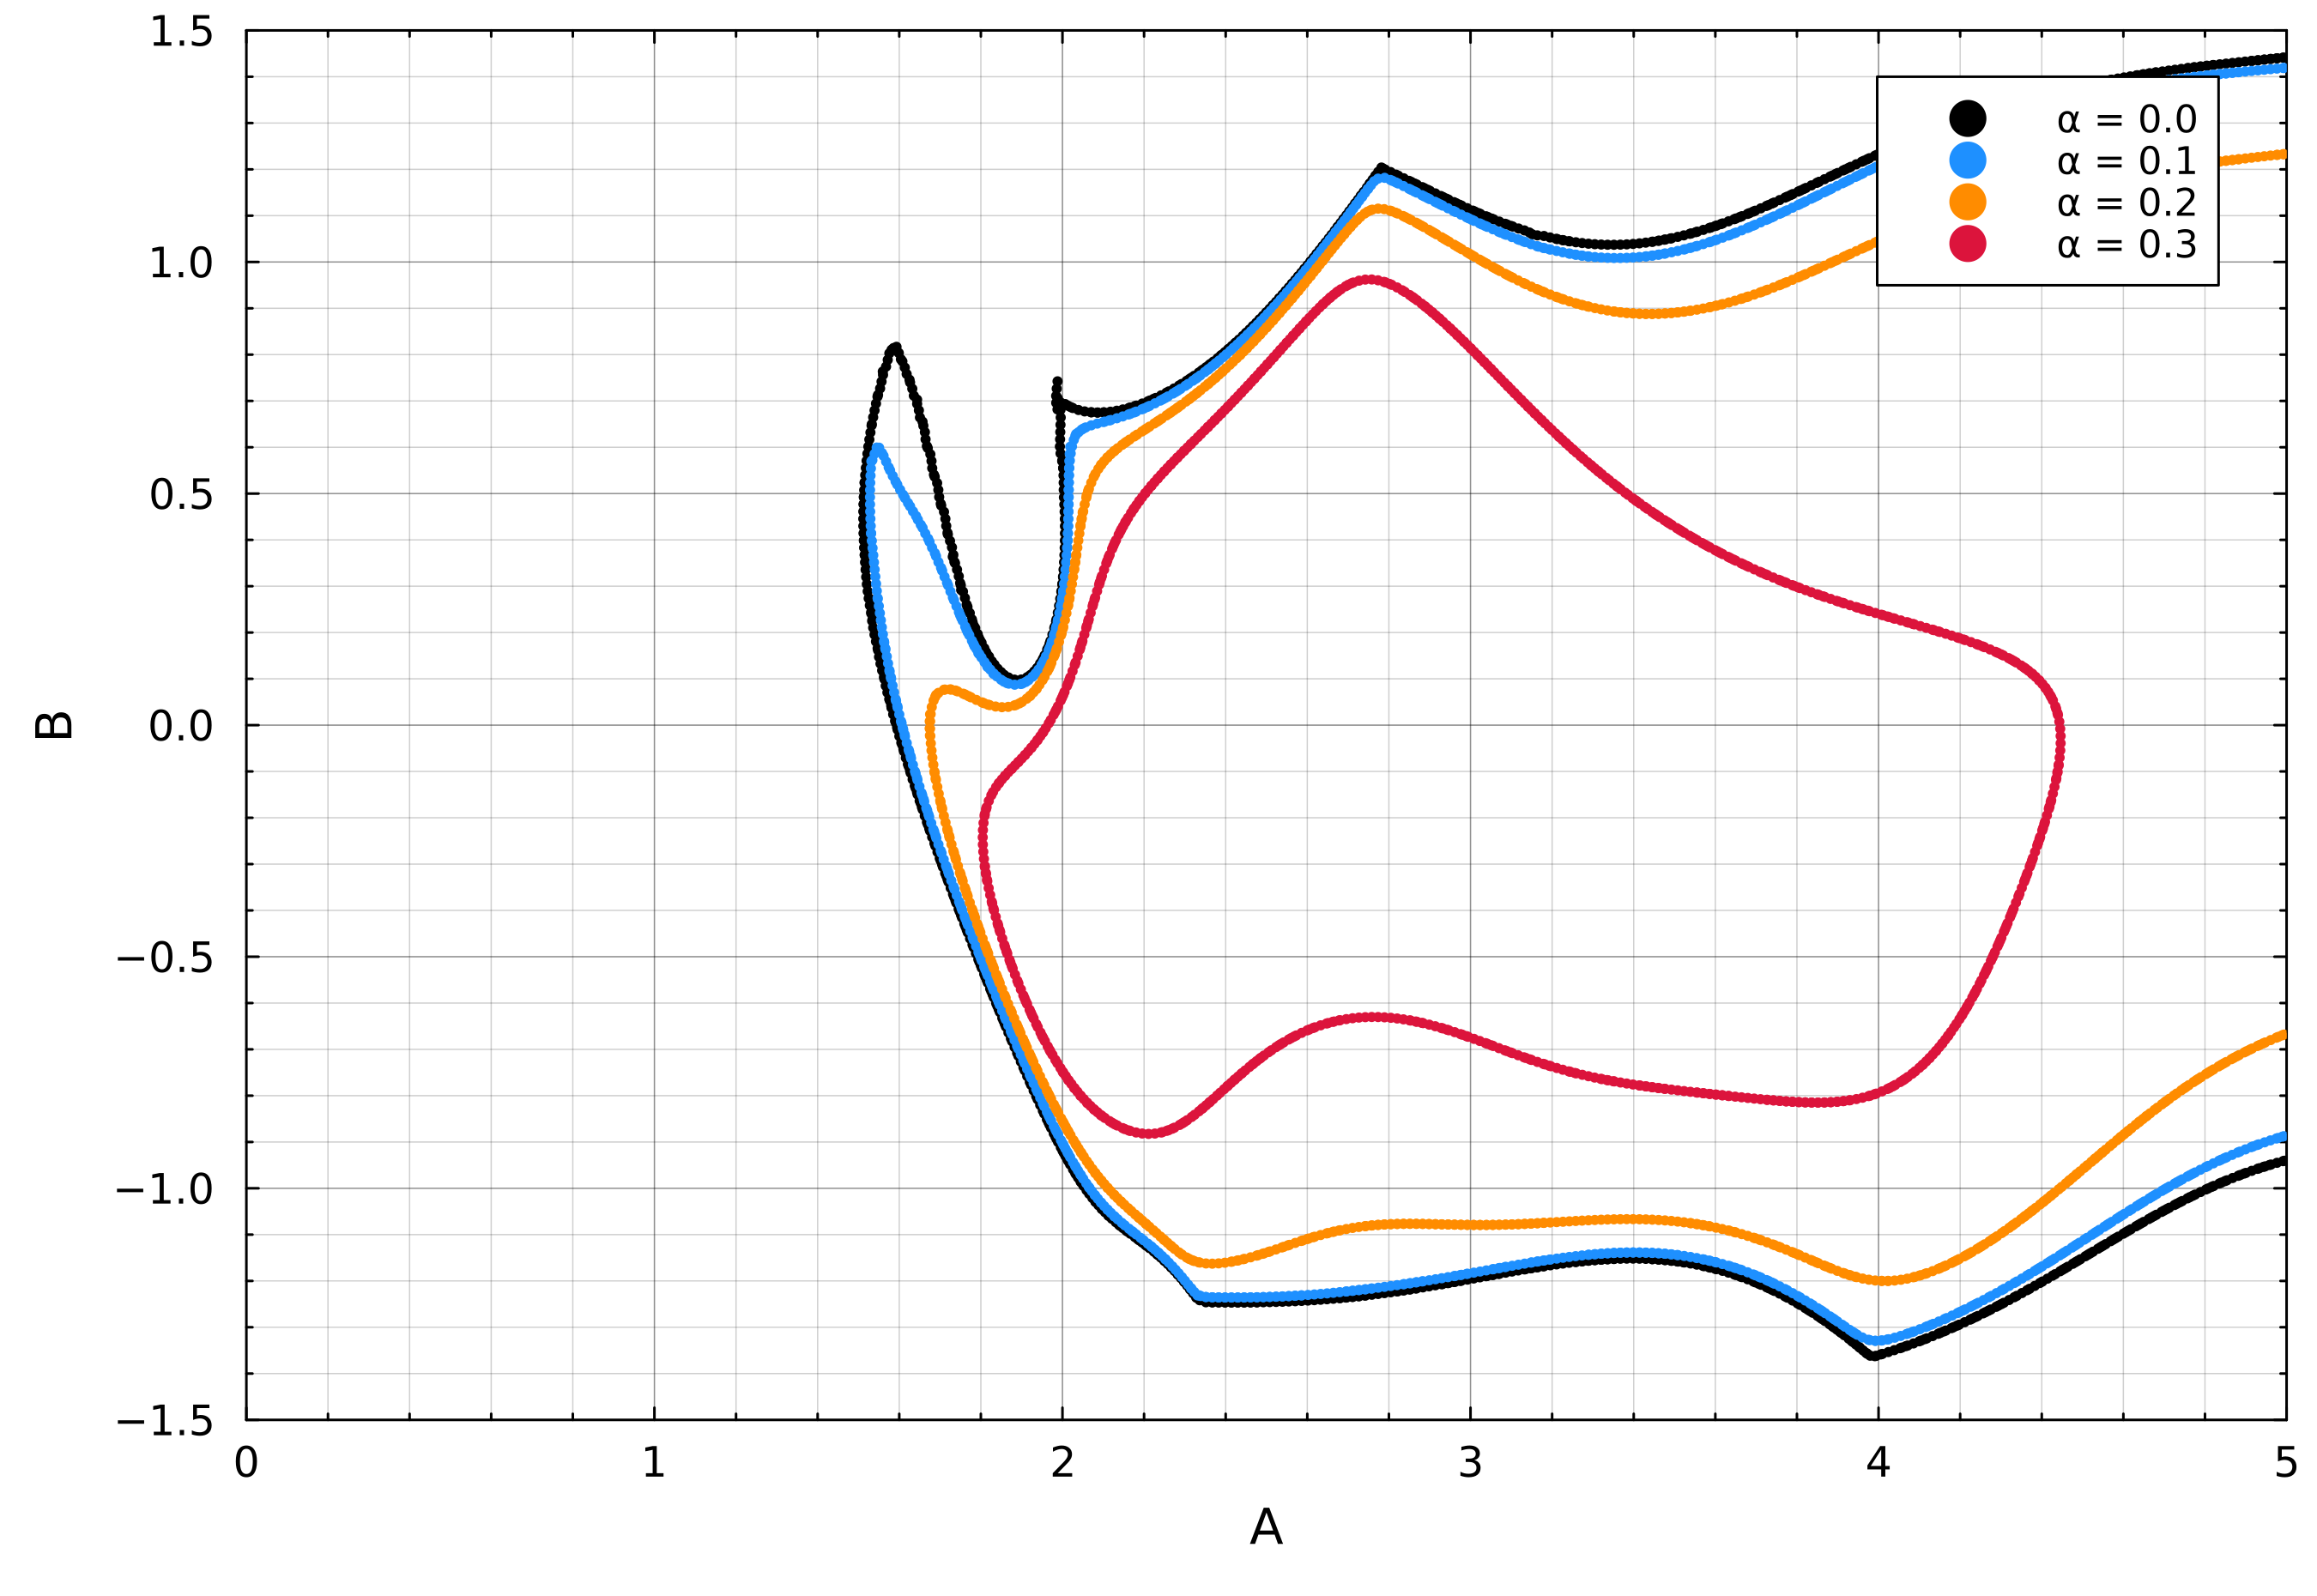
\includegraphics[width=0.72\textwidth]{images/fig1_sykora_fig4_repro.png}
    \caption{Second-moment stability boundaries of the stochastic delayed Mathieu equation in the $(A,B)$ plane for multiplicative noise intensities $\alpha \in \{0, 0.1, 0.2, 0.3\}$ ($\epsilon=2$, $\zeta=0.1$, $\tau=2\pi$, period $4\pi$, $p=40$, $q=2$); reproduction of Fig.~4 of \cite{Sykora2020a}. The stable region shrinks monotonically with increasing noise.}
    \label{fig:mathieu}
\end{figure}

\subsection{Work-Precision and Memory Scaling}
The scaling claim of Section \ref{sec:mf_algo} is verified directly by evaluating the \emph{same} discrete operator along both routes: the classical path assembles the explicit period product of Eq.~\eqref{eq:period_product} (sparse single-step factors, explicitly multiplied into a densifying accumulator) and calls a sparse eigensolver on the result, while the MF path evaluates only operator actions inside the Krylov iteration. Figure~\ref{fig:wp_ultra} reports wall-clock time, memory, and accuracy on the fully time-periodic stochastic delayed Mathieu benchmark (all coefficients $T$-periodic, present and delayed multiplicative noise; $q=2$; single-threaded, one BLAS thread; timings are minima over repeated runs after JIT warm-up; all CPU results in this paper were obtained on a dual-socket Intel Xeon Gold 6154 workstation ($2\times18$ cores, $3.0\,\mathrm{GHz}$, $192\,\mathrm{GB}$ RAM), Julia 1.12, KrylovKit with Krylov dimension 15; single-core unless a thread count is stated). The memory metric is the \emph{cumulative solver allocation} reported by the runtime --- a robust, reproducible proxy that upper-bounds the peak working set; the peak footprint itself scales as $\mathcal{O}(p^4)$ for the explicit product (one densifying $D\times D$ accumulator) versus $\mathcal{O}(p^2)$ for MF. Panel (c) confirms that the two routes are algebraically identical --- the error curves coincide point-by-point --- so the comparison isolates pure implementation cost. The classical route follows the predicted $\mathcal{O}(p^4)$ growth in time (the cumulative allocation grows one power faster, $\mathcal{O}(p^5)$, since $p$ products of $\mathcal{O}(p^4)$ objects are formed): at $p = 192$ it requires $384\,\mathrm{s}$ and allocates $386\,\mathrm{GB}$ cumulatively, against $0.030\,\mathrm{s}$ and $22\,\mathrm{MB}$ for the multiplication-free route --- a measured factor of $1.3\times10^{4}$ in time and $1.8\times10^{4}$ in allocation --- and becomes infeasible shortly above this resolution. The MF route continues along its $\mathcal{O}(p^2)$ trend to $p = 2048$ (and to $p = 4096$ in the GPU experiments of Appendix~\ref{app:gpu}) on the same machine. Figure~\ref{fig:wp_ultra} also includes the natural \emph{intermediate} classical formulation --- the sparse single-step recursion applied $p$ times per operator action, with the covariance copied at each step, which avoids the explicit product without any of the new machinery --- whose $\mathcal{O}(p^3)$ per-application cost is confirmed by the data: at $p = 1024$ it takes $507\,\mathrm{s}$ against $1.2\,\mathrm{s}$ for MF, an advantage of one power of $p$ that keeps growing with resolution. The Arnoldi eigensolve (KrylovKit, Krylov dimension 15, relative tolerance $10^{-12}$, no restart needed) converges within a single Krylov factorization --- $15$ operator applications --- for \emph{every} $p$ and every method in the sweep (identical operators, identical spectra), so the per-application cost governs the end-to-end scaling in all cases. The dominant eigenvalue of $\mathcal{H}$ is real and positive in all our experiments, as expected for a map that preserves the cone of positive-semidefinite matrices; no preconditioning is used anywhere in this paper.

\begin{figure}[ht!]
    \centering
    
\includegraphics[width=0.92\textwidth]{images/wp_ultra.png}
    \caption{Three evaluations of the identical second-moment operator (fully periodic stochastic delayed Mathieu, $q=2$): explicit period product (black), single-step recursion with copy (gray dashed, $\mathcal{O}(p^3)$), and multiplication-free (red, $\mathcal{O}(p^2)$). (a) Wall-clock time with $p^2$/$p^4$ guides; (b) cumulative solver allocation; (c) error vs resolution --- the curves coincide, confirming algebraic identity; (d) error vs cost. At $p=192$ the measured advantage over the explicit product is $1.3\times10^4$ in time and $1.8\times10^4$ in allocation; over the step recursion it is $\approx 420\times$ at $p=1024$ and grows linearly with $p$.}
    \label{fig:wp_ultra}
\end{figure}

\subsection{Delayed PD Control of the Stochastic Mathieu Oscillator: the Effect of Rough Reads and the IBP Remedy}
\label{sec:results_pd}
To isolate the order-limiting mechanism of Section \ref{sec:ibp} on the canonical benchmark, we extend the delayed Mathieu equation by a time-periodic delayed PD control law and strong multiplicative noise:
\begin{equation}
\label{eq:pd_mathieu}
\ddot q + 2\zeta \dot q + \big(\delta + \epsilon \cos \Omega t\big) q
= k_P(t)\, q(t-\tau) + k_D(t)\, \dot q(t-\tau)
+ \big[\alpha\, q + \beta\, q(t-\tau)\big] \dot W(t),
\end{equation}
with periodic gains $k_P(t) = k_{P0}\,(1 + \kappa_P \cos \Omega t)$ and $k_D(t) = k_{D0}\,(1 + \kappa_D \cos \Omega t)$. In first-order form the delayed matrix $\mathbf{B}(t)$ acquires a non-zero \emph{velocity} column through $k_D$, which is exactly a rough delayed read: the noise drives the velocity row through $\alpha, \beta \ne 0$. In the reported study $\zeta = 0.05$, $\delta = 1$, $\epsilon = 0.8$, $\Omega = 2\pi$, $\tau = 1$, $k_{P0} = 0.40$, $\kappa_P = 0.3$, $k_{D0} = 0.45$, $\kappa_D = 0.4$, $\alpha = 0.5$, $\beta = 0.35$ (deliberately strong gains and noise so that the convergence is measurable over several decades). The reference value $\rho_{\mathrm{ref}} = 1.324866438112$ is self-converged within the highest-order scheme ($\Delta = 4.6\times10^{-11}$ between its two finest resolutions) and independently confirmed to $9.4\times 10^{-13}$ by a fine-grid method-of-steps solver for the two-time covariance kernel (second-order accurate, Richardson-extrapolated) that shares no discretization machinery with the methods under test.

Figure \ref{fig:pd_orders} summarizes the measured convergence of $\rho(\mathcal{H})$ for three treatments of the delayed coupling, all using Gauss--Legendre collocation with $S=3$ stages (nominal order six). The sampling-based treatment collapses to a clean second order (measured local rates $2.03, 2.01, 2.00, 2.00, 2.00$) --- the rough-read ceiling --- while the integrated-history treatment restores the full nominal order (rates $6.06, 6.00, 5.97, 6.07$), reaching $|\rho - \rho_{\mathrm{ref}}| \approx 8\times 10^{-12}$ at just $p=24$ steps per period. The IBP reformulation preserves the restored order and further reduces the error constants by a factor of $2$--$3$; at $S=4$ stages the IBP variant attains $10^{-9}$ accuracy at $p=4$, i.e.\ with four steps per period. For first-order systems in which the delayed drift reads the rough component itself (so that no smooth antiderivative is available in the state), a residual $\mathcal{O}(\Delta t^4)$ term remains; this case is outside the scope of the present paper (cf.\ the block-local outlook in Section \ref{sec:ibp}).

\begin{figure}[ht!]
    \centering
    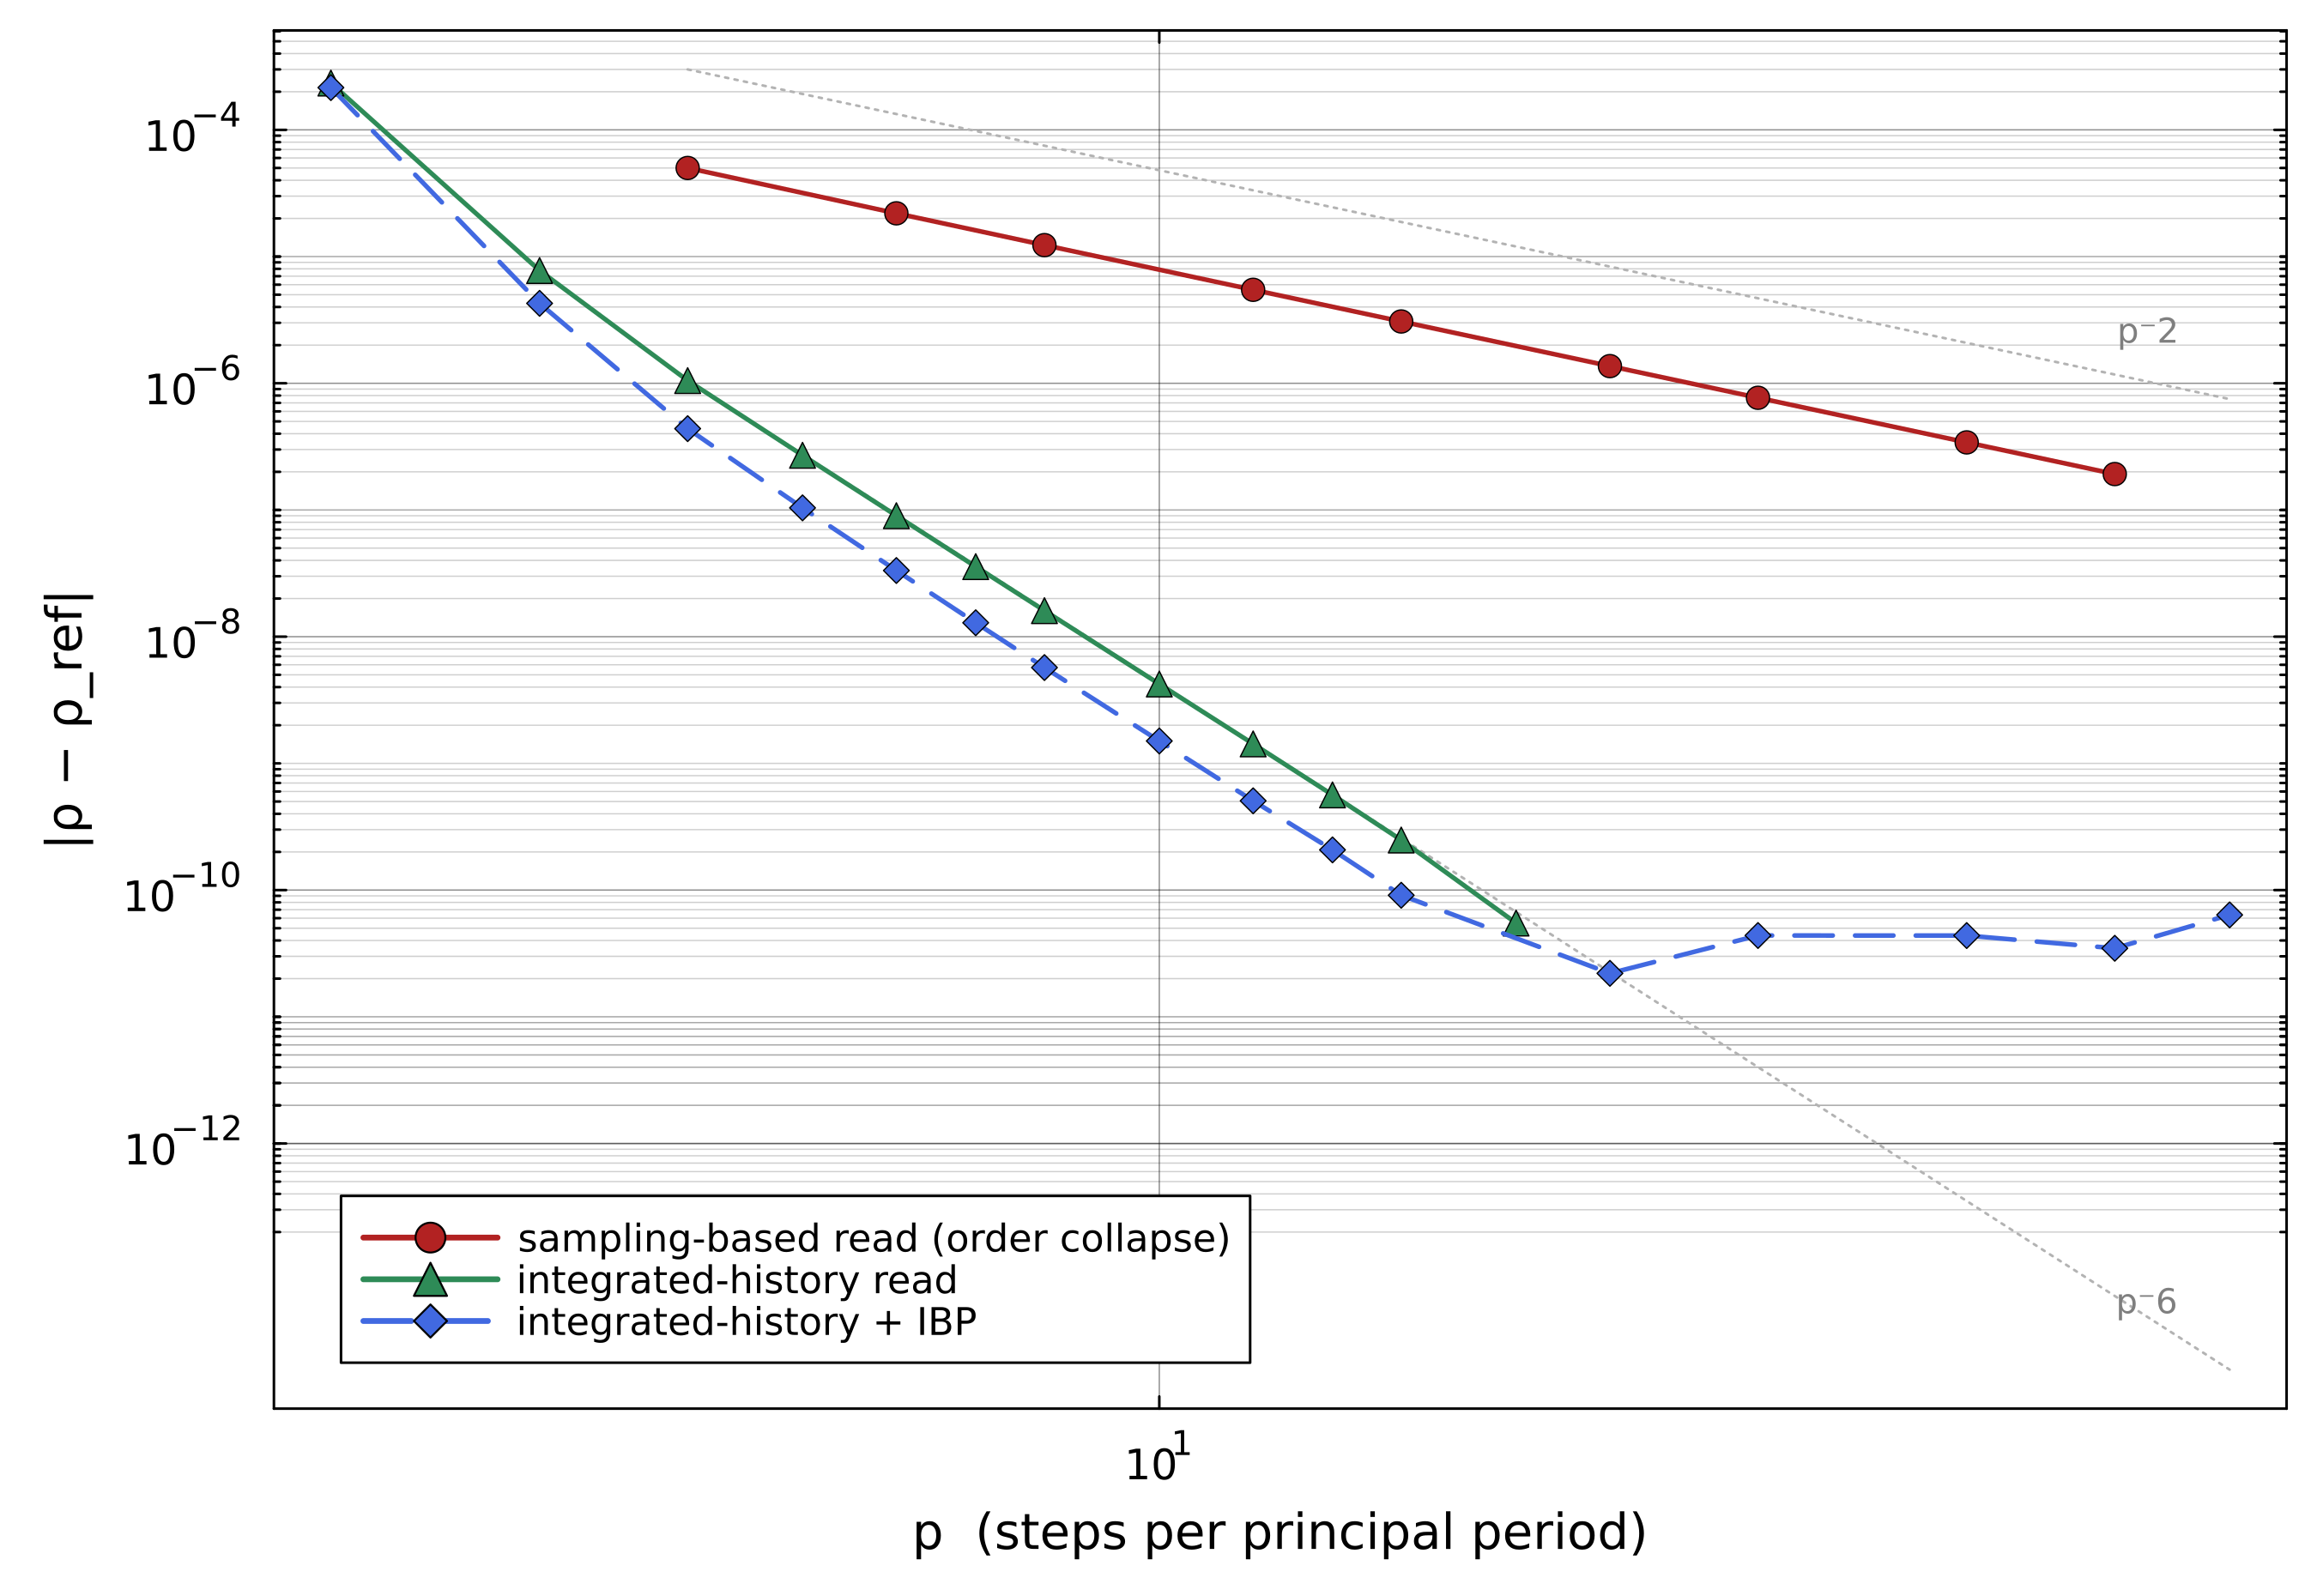
\includegraphics[width=0.62\textwidth]{images/pd_mathieu_orders.png}
    \caption{Convergence of $\rho(\mathcal{H})$ for the PD-controlled stochastic Mathieu equation \eqref{eq:pd_mathieu} ($S=3$ Gauss--Legendre stages). Sampling the delayed-velocity term collapses the order to $\mathcal{O}(\Delta t^2)$; carrying it as an integrated-history quantity restores the nominal sixth order; the IBP reformulation additionally reduces the error constants. Reference certified to $9.4\times10^{-13}$ by an independent fine-grid two-time-covariance solver.}
    \label{fig:pd_orders}
\end{figure}

Figure \ref{fig:grand_orders} places all methods on a common error--resolution diagram for the same problem: the classical stochastic semi-discretization (orders $q=2$ and $q=4$ of the underlying deterministic scheme) against the integrated-history collocation engine with $S = 1,\dots,5$ Gauss--Legendre stages, each with and without the IBP reformulation. Two observations stand out. First, the classical method converges at first order in the second moment regardless of $q$ --- the measured slopes are $0.99$ for both $q=2$ and $q=4$ over more than two decades of resolution --- so no amount of refinement of the deterministic scheme lifts the stochastic order. Second, the collocation family realizes its nominal order $2S$ until it meets the accuracy floor of the iterative eigensolver ($\sim 10^{-11}$): measured slopes are $2.0$ ($S=1$), $4.1$--$4.6$ ($S=2$), and $\approx 6$ ($S=3$) with the $S=4,5$ curves starting at $10^{-9}$ already at $p=4$ and reaching the floor by $p \approx 12$. In practical terms, the $S=4$ scheme at $p=8$ is more accurate than the classical scheme would reach at $p = 10^4$ (extrapolating its measured first-order trend).

\begin{figure}[ht!]
    \centering
    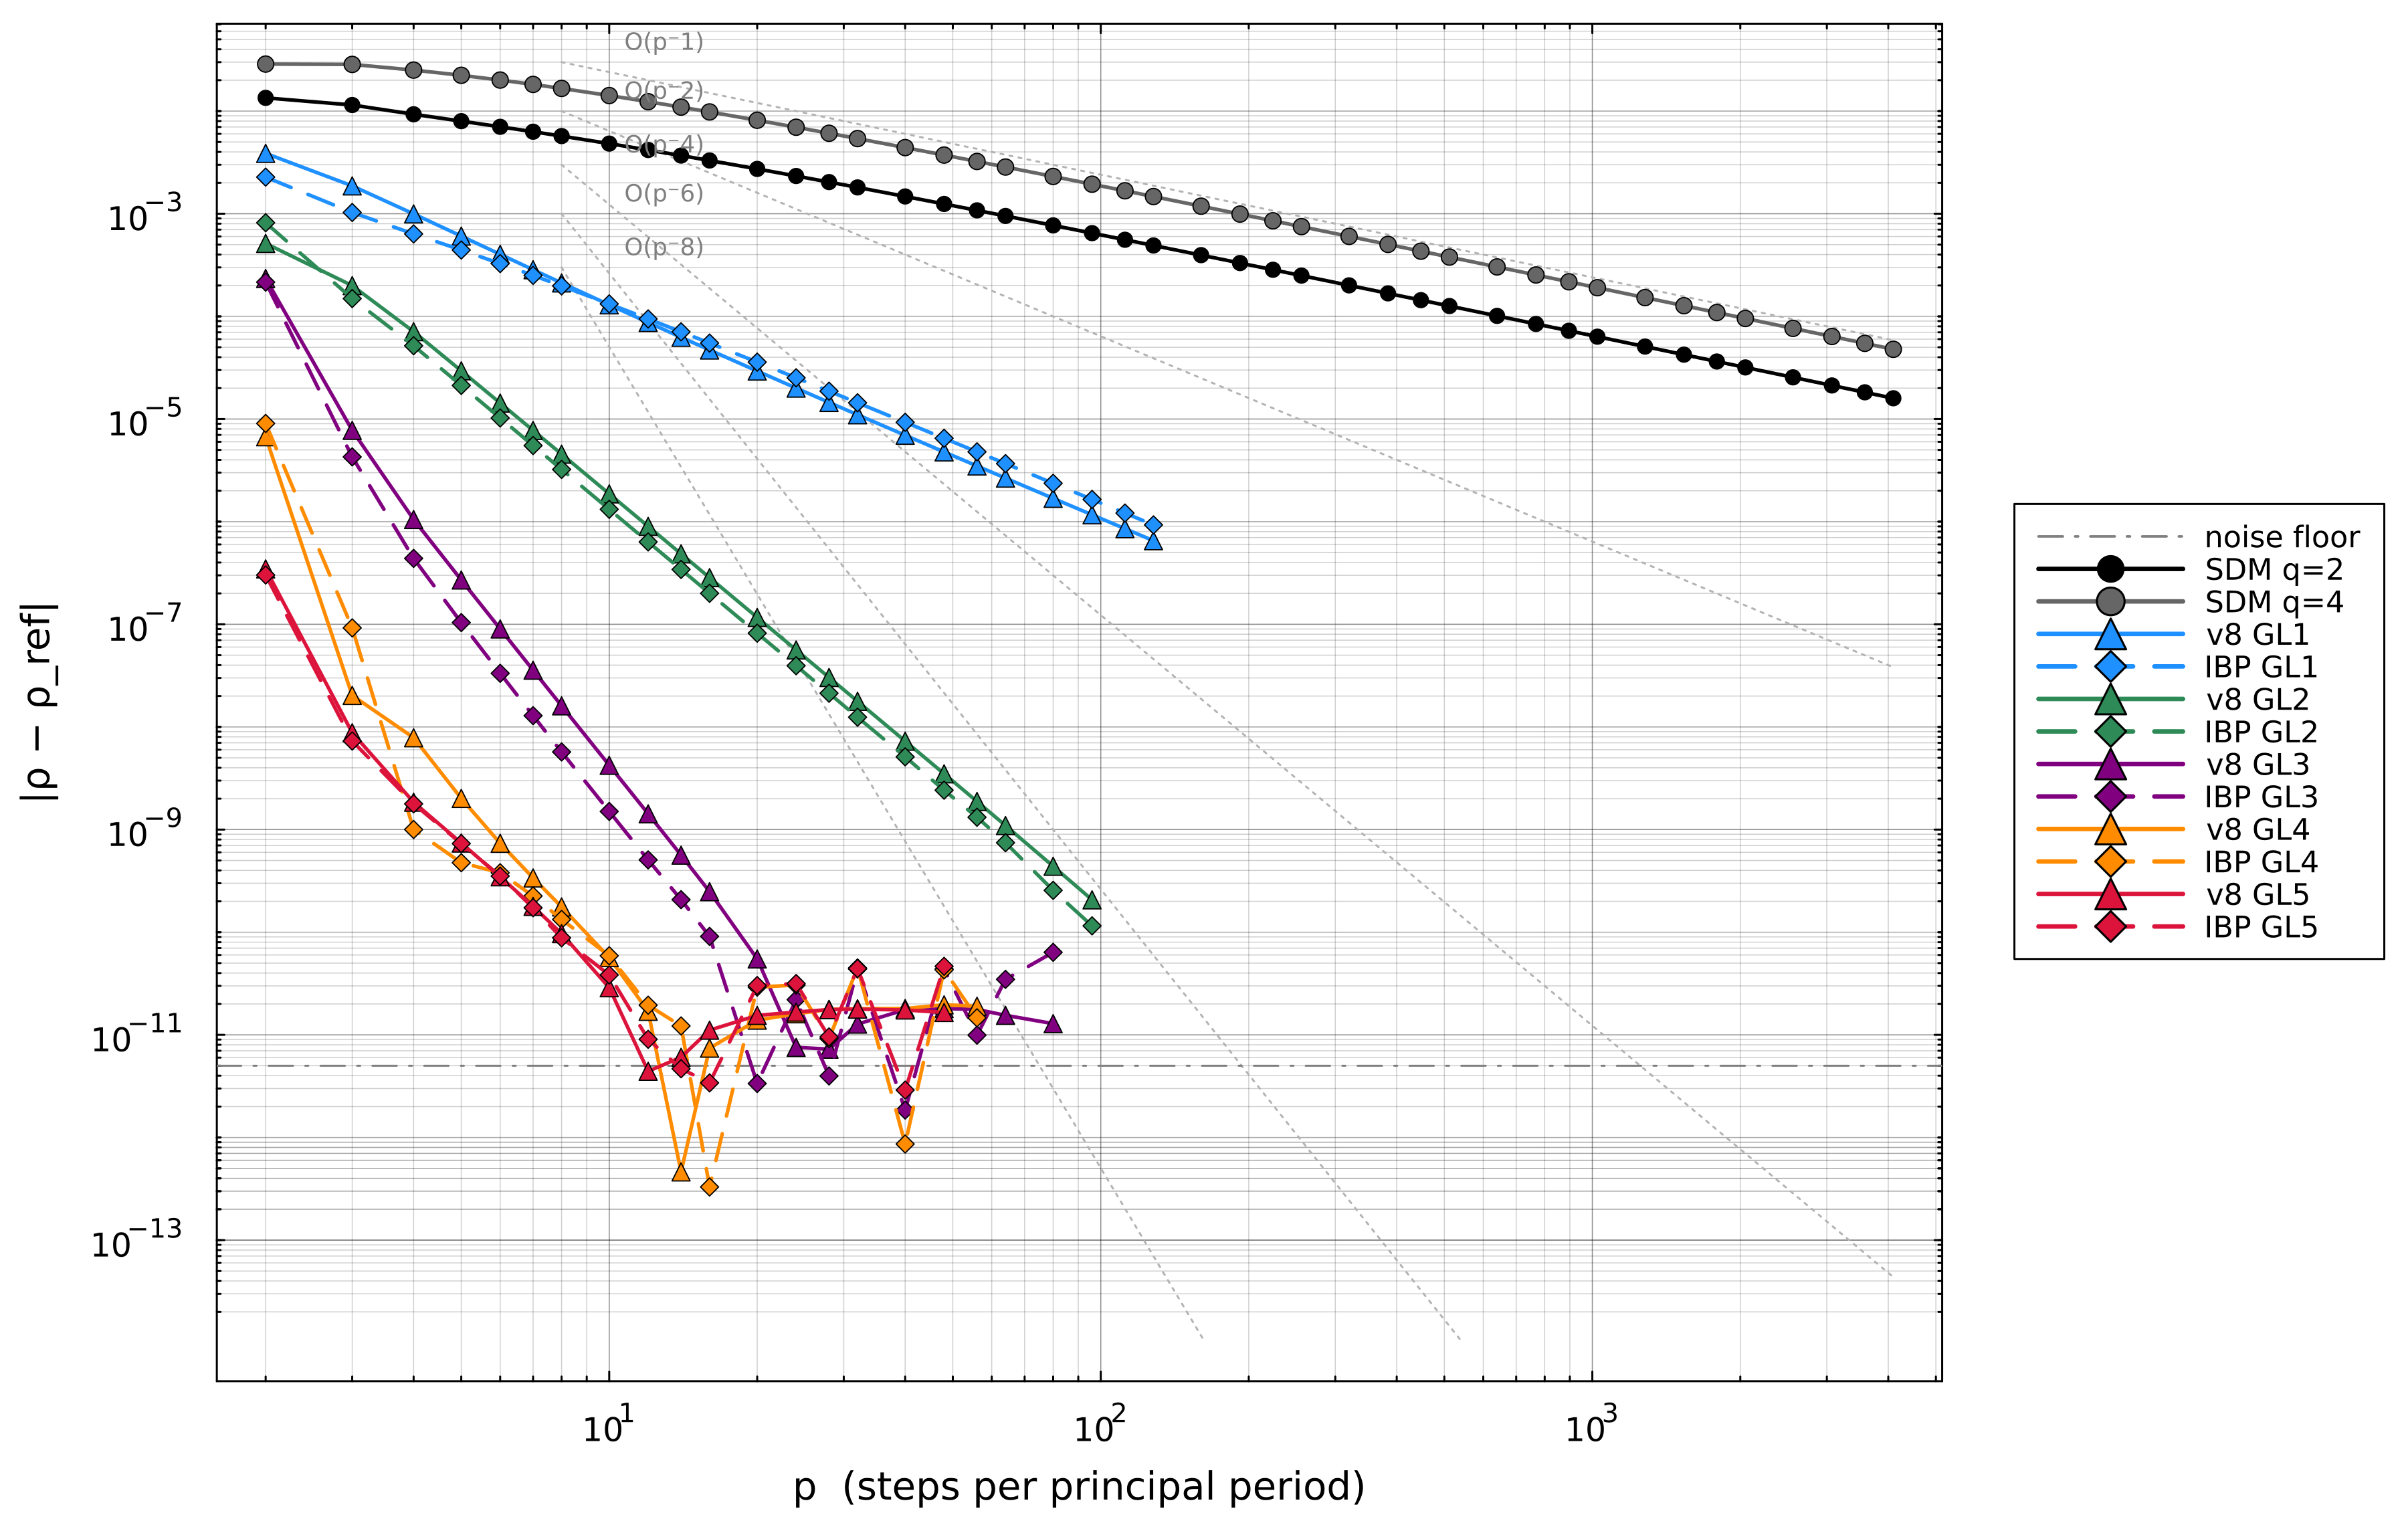
\includegraphics[width=0.85\textwidth]{images/grand_orders_pub.png}
    \caption{Error--resolution diagram for the PD-controlled stochastic Mathieu equation \eqref{eq:pd_mathieu}: classical stochastic semi-discretization (SDM, $q=2,4$) vs the integrated-history collocation engine (GL$S$, $S=1,\dots,5$; solid) and its IBP variant (dashed). Dotted guides indicate slopes $p^{-1}$ to $p^{-8}$; curves are truncated where they reach the eigensolver accuracy floor (dash-dotted line). The classical method is first-order in the second moment for any $q$; the collocation family attains its nominal order $2S$.}
    \label{fig:grand_orders}
\end{figure}

Convergence order alone does not settle which method is cheapest for a target accuracy, since higher-order blocks carry more degrees of freedom per step. Figure~\ref{fig:triple} therefore reports the full work--precision picture for \emph{both} deliverables of the method: the Floquet stability indicator $\rho(\mathcal{H})$ (top row) and the stationary second moment $\operatorname{Var}(q)=\mathbf{M}^*_{q,q}$ (bottom row), the latter computed on a stable variant of Eq.~\eqref{eq:pd_mathieu} (damping and gains reduced so that $\rho(\mathcal{H})\approx0.77$ and a bounded stationary variance exists, with an additive load-noise source added so that variance is non-trivial; reference $\operatorname{Var}_{\mathrm{ref}}=0.18675690782$, self-converged to $10^{-11}$; unlike $\rho_{\mathrm{ref}}$ it carries no independent-solver certificate). Three views are shown: error versus resolution $p$ (left), wall-clock cost versus $p$ (middle), and the decisive error-versus-cost tradeoff (right). Per step the classical operator is the cheapest (middle column), but because it is stuck at first order it must take $p\sim 10^3$--$10^4$ steps to reach even $10^{-5}$, whereas a fourth- or fifth-stage collocation scheme reaches the solver floor ($\sim10^{-10}$) in a few tenths of a second at $p\lesssim 12$. On the accuracy-per-cost axis (right column) the high-order schemes are consequently three to five orders of magnitude more accurate than the classical method at equal wall-clock time, for the stationary variance exactly as for the spectral radius.

\begin{figure}[ht!]
    \centering
    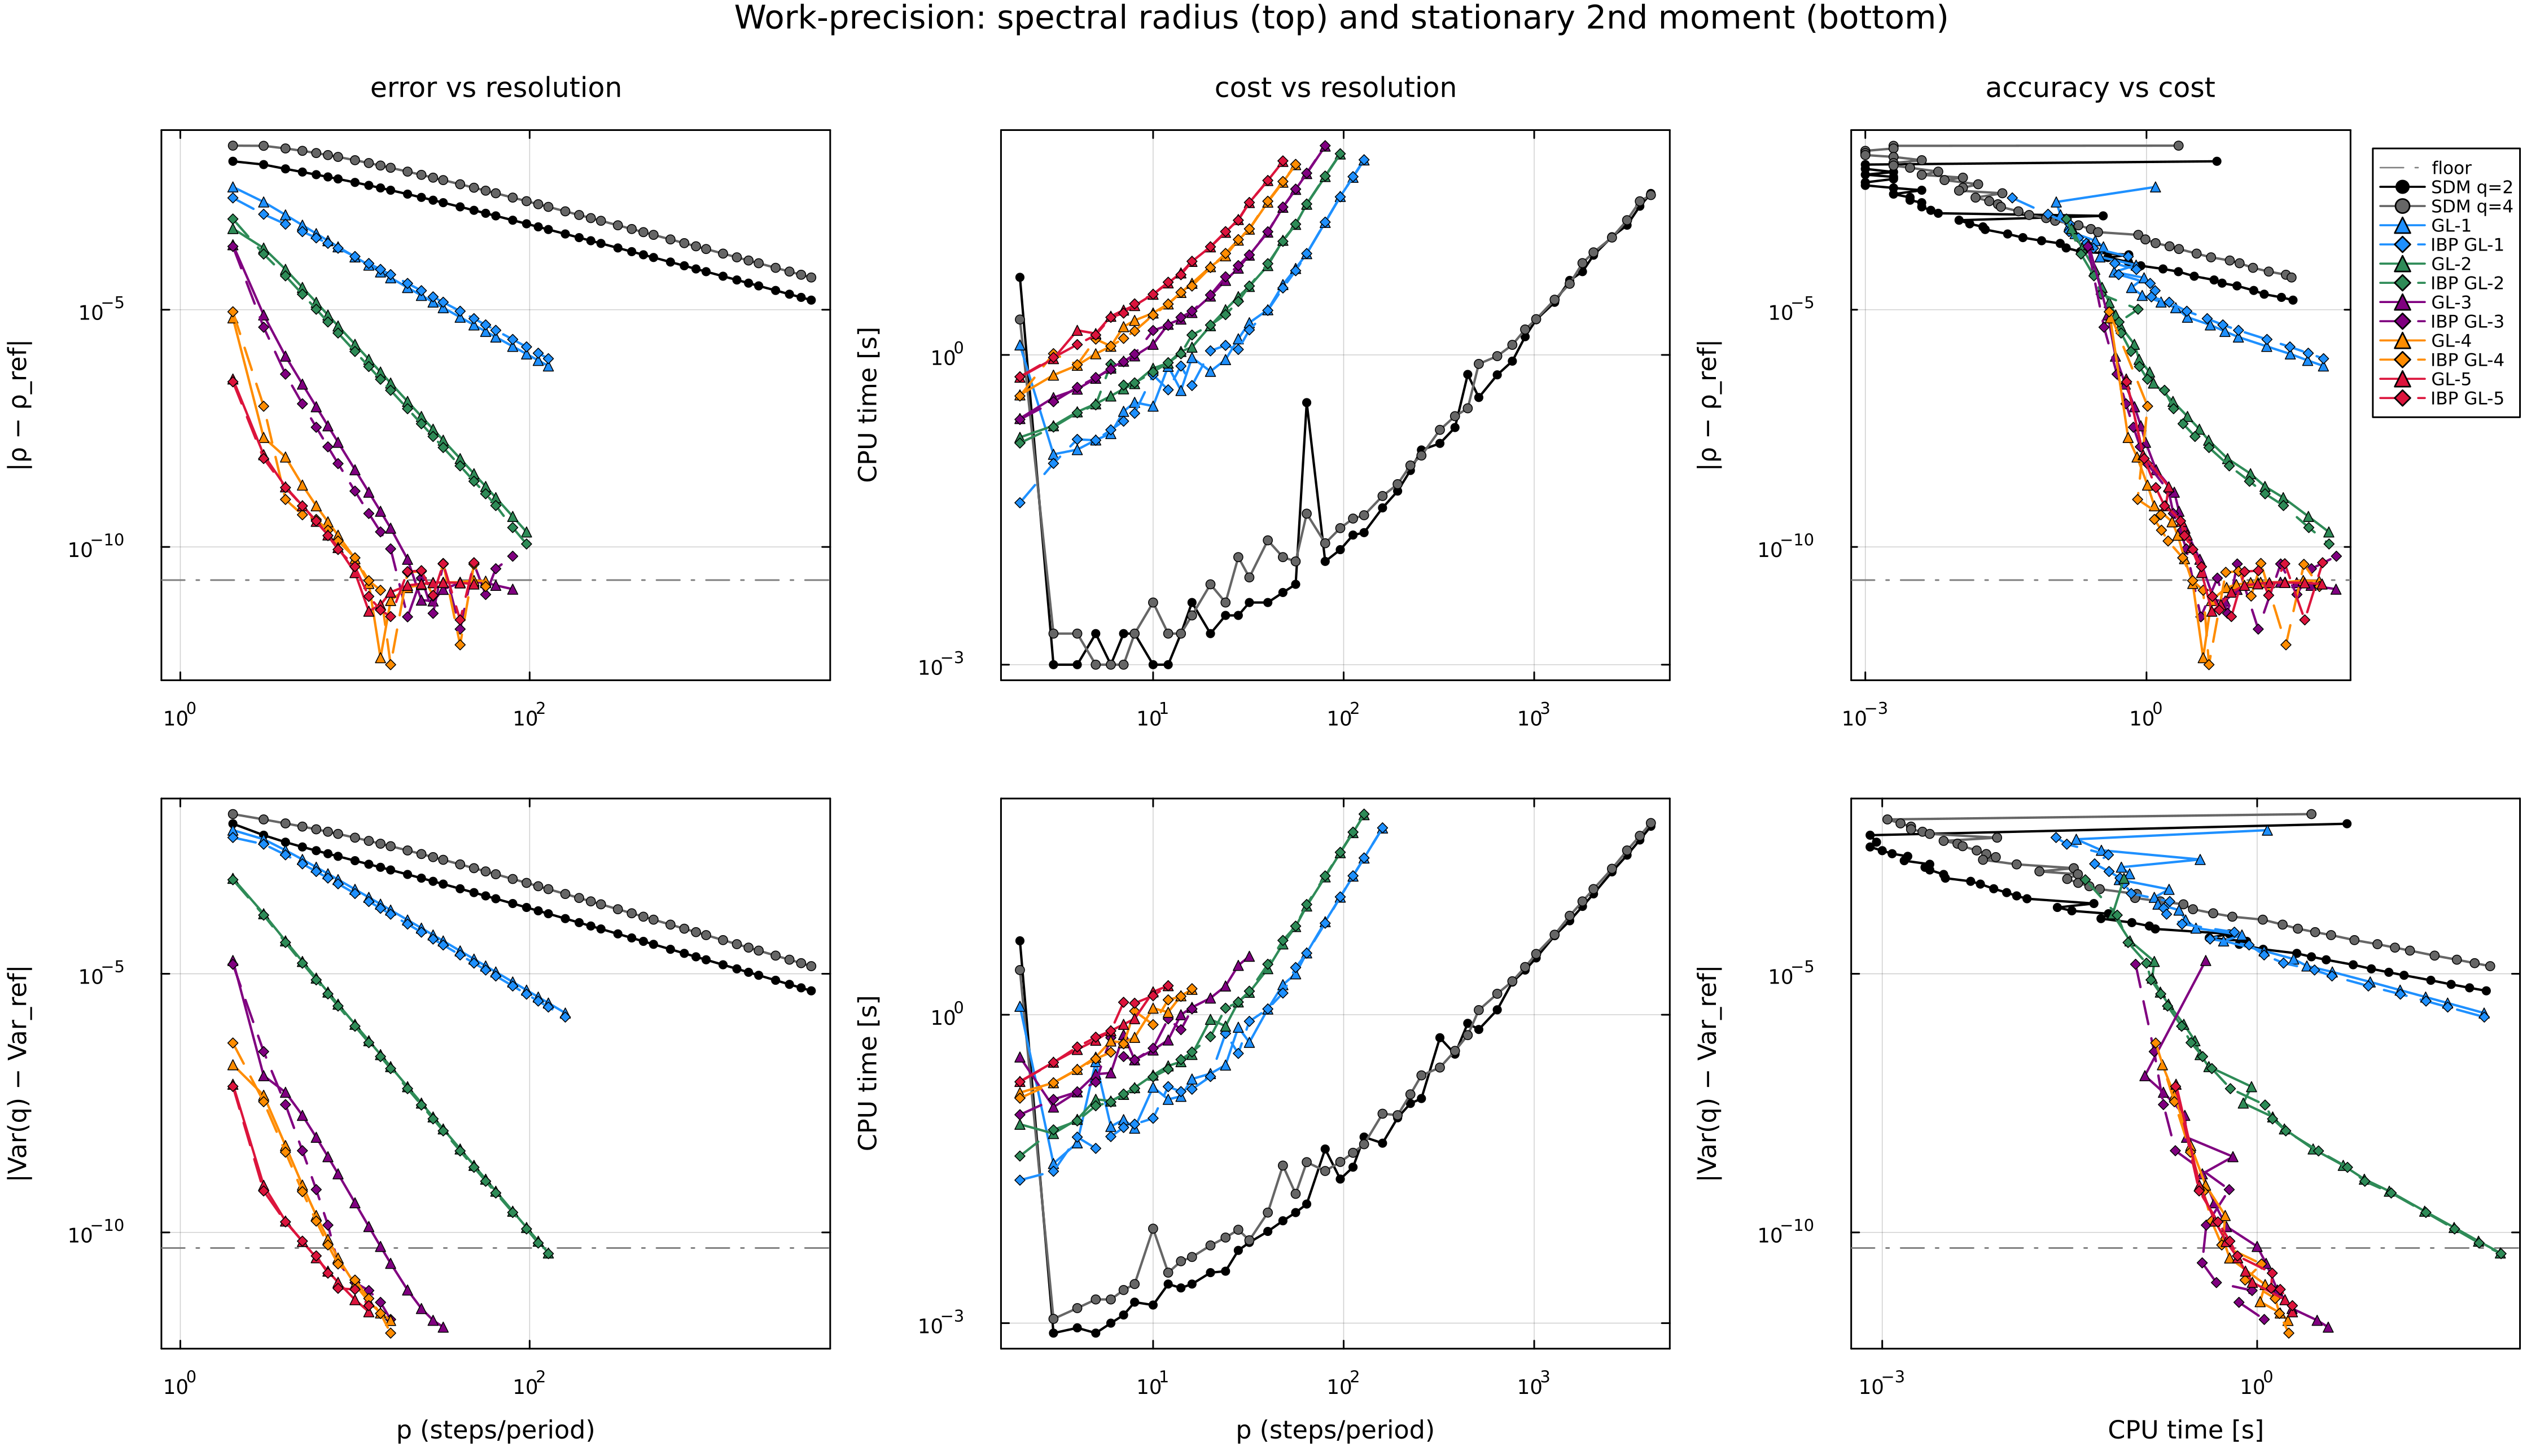
\includegraphics[width=0.95\textwidth]{images/grand_triple.png}
    \caption{Work--precision diagrams for the two second-moment deliverables on the PD-controlled stochastic Mathieu problem: Floquet spectral radius $\rho(\mathcal{H})$ (top) and stationary variance $\operatorname{Var}(q)$ (bottom). Columns: error vs resolution $p$; CPU time vs $p$; error vs CPU time. Same method set and styling as Fig.~\ref{fig:grand_orders}. The rightmost column is the practical figure of merit --- accuracy per unit wall-clock time --- on which the high-order collocation schemes dominate the classical semi-discretization by several orders of magnitude for both quantities.}
    \label{fig:triple}
\end{figure}

Since the collocation blocks store $2S+2$ history sub-states per step while the classical scheme stores one, resolution $p$ alone is not a storage-fair comparison axis. Figure~\ref{fig:stored} therefore replots the error of both quantities against the number of \emph{stored history sub-points per period}, $N = p\,(2S+2)$ for GL-$S$ and $N = p$ for the classical scheme, next to the plain resolution axis. The rescaling shifts each collocation curve right by its factor $2S+2$ and leaves the classical curves unchanged. Two conclusions follow. At low accuracy targets the picture tightens considerably: per stored point, the $S=1$ scheme no longer outperforms the classical method --- its second-order gain does not pay for its fourfold storage. At tight tolerances the ordering is unaffected: the $S \ge 3$ schemes reach $10^{-10}$ with $N \approx 10^2$ stored sub-points, where the classical first-order scheme would require $N$ of order $10^{8}$. High order wins not because it stores more information per step, but because of the slope.

\begin{figure}[ht!]
    \centering
    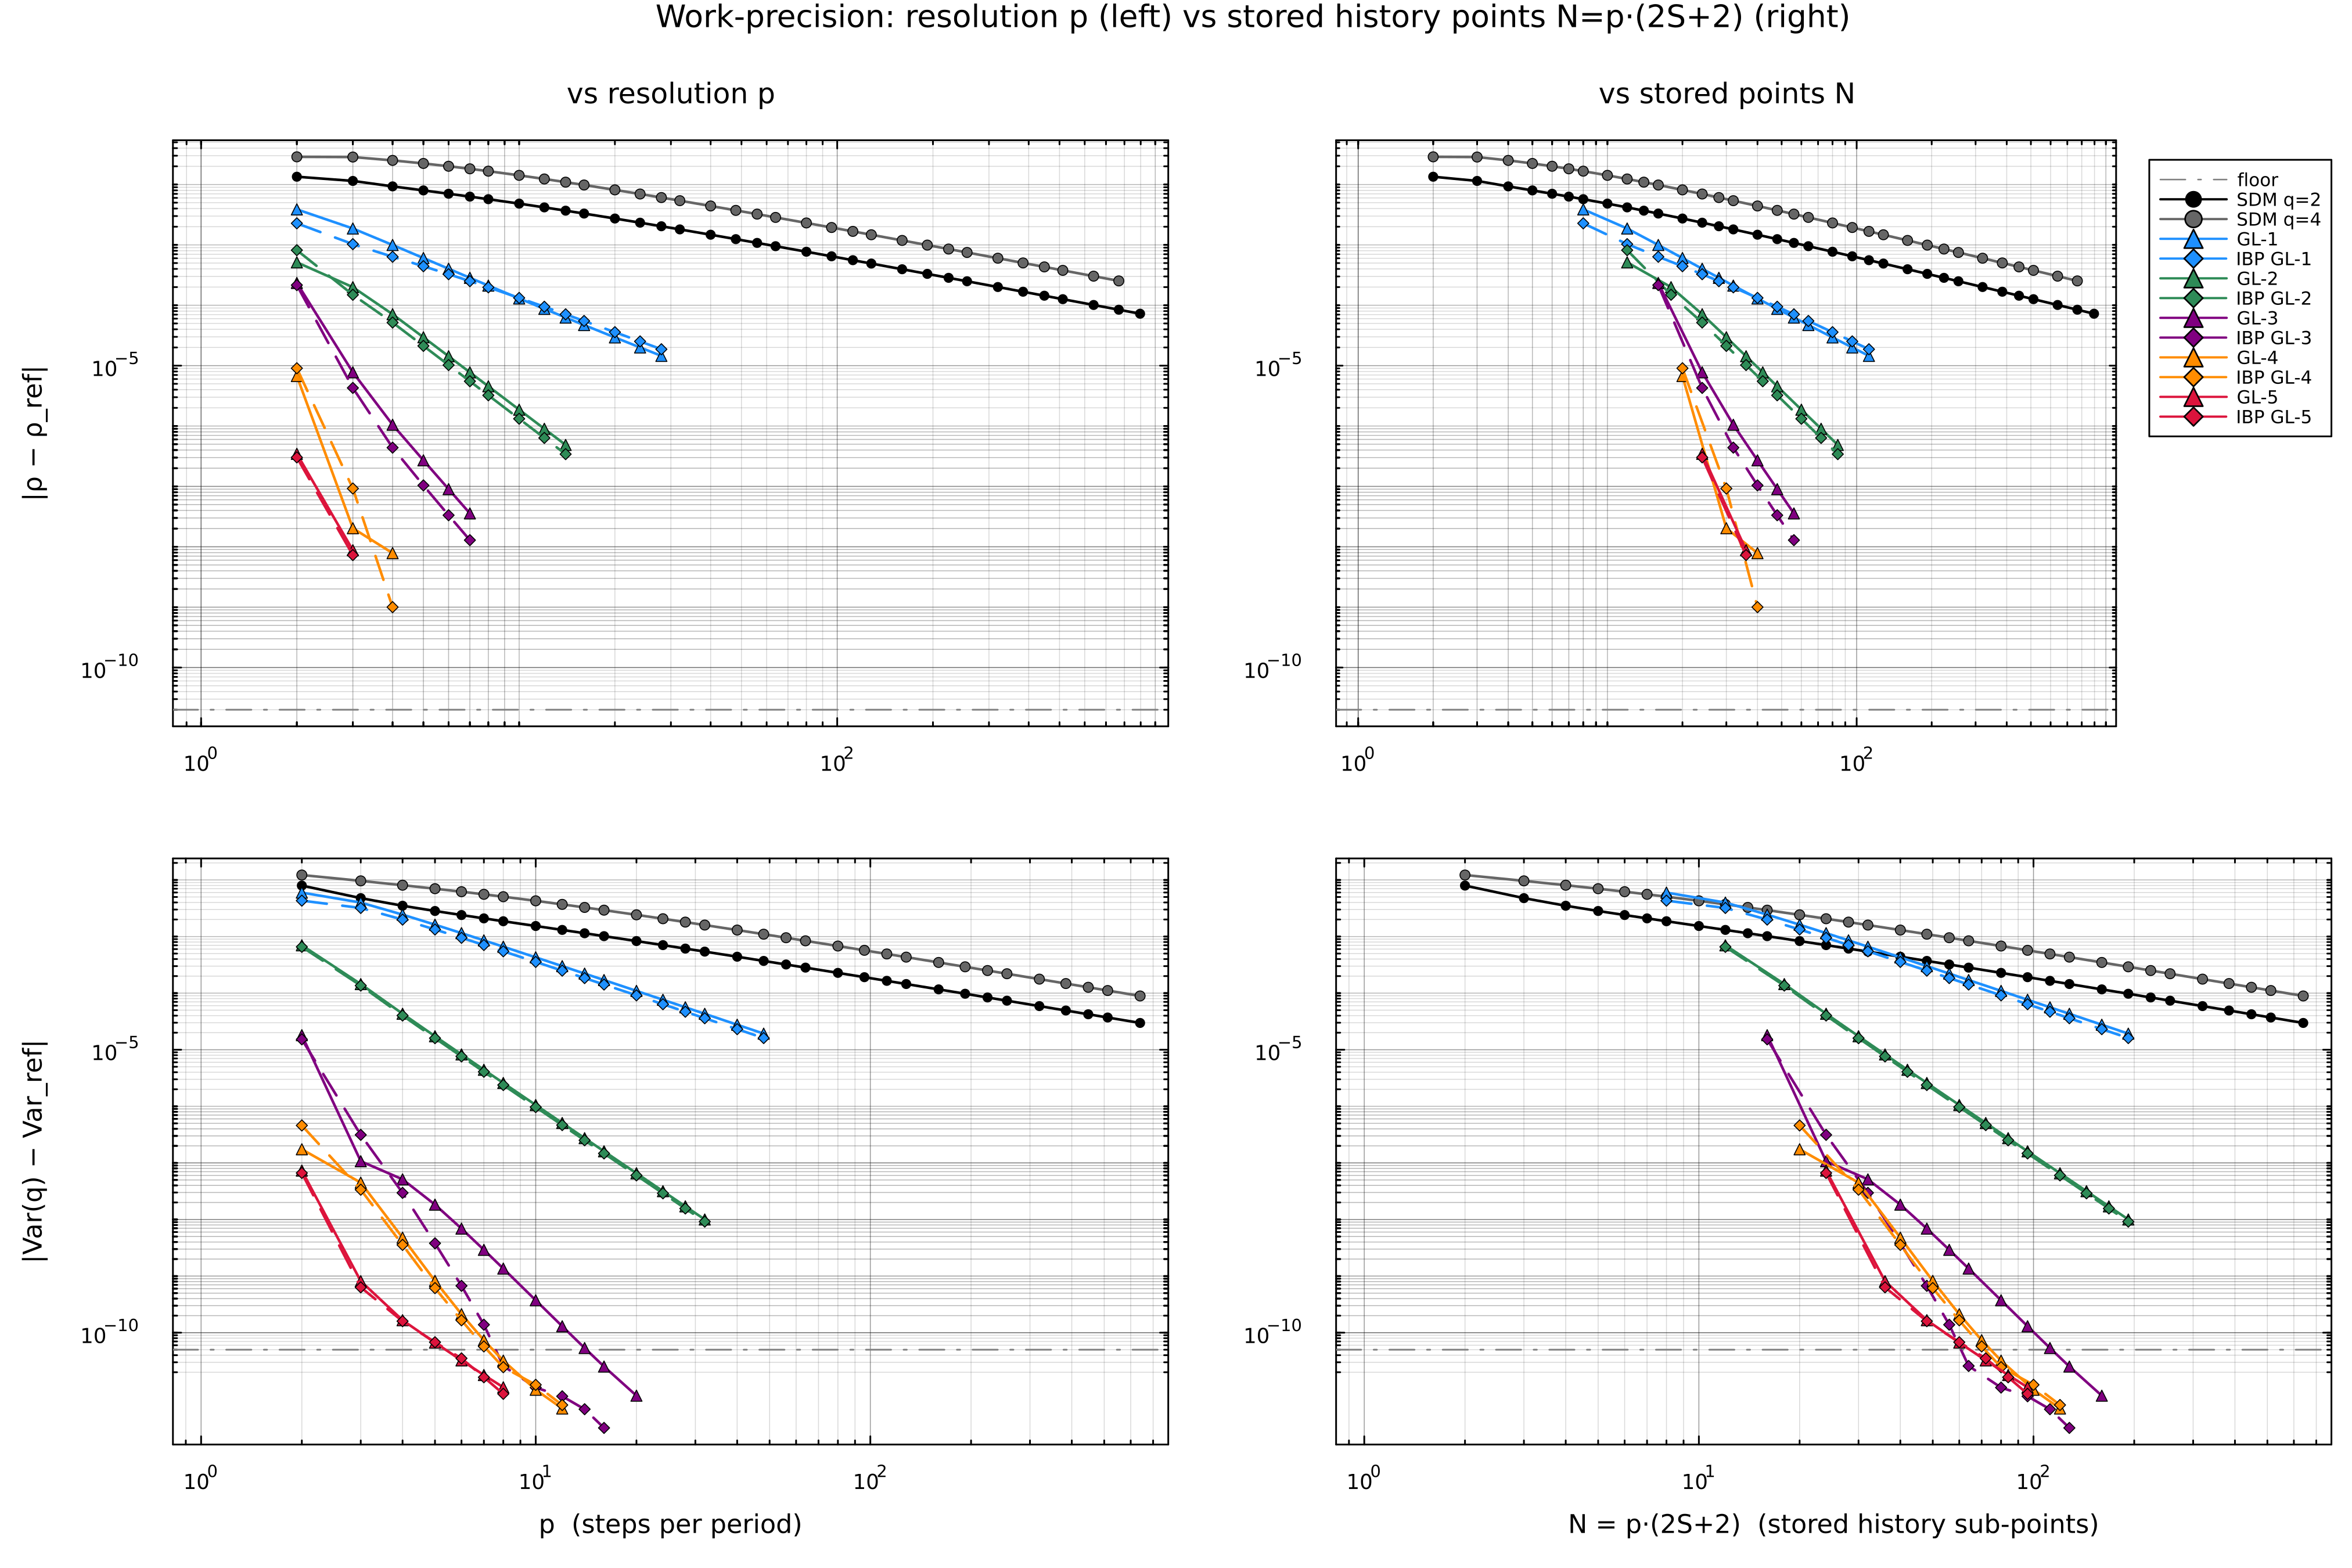
\includegraphics[width=0.88\textwidth]{images/grand_stored.png}
    \caption{Work--precision replotted against stored history sub-points $N$ (right column) next to the resolution axis $p$ (left column), for the spectral radius (top) and the stationary variance (bottom). GL-$S$ stores $2S+2$ sub-states per step ($N = p\,(2S+2)$); the classical scheme stores one ($N=p$). Per stored point the $S=1$ scheme loses its advantage over the classical method, while the $S\ge3$ schemes retain a many-orders-of-magnitude lead at tight tolerances.}
    \label{fig:stored}
\end{figure}

\subsection{Time-Varying Delay: Measured Orders on the SSV Turning Model}
\label{sec:results_tvd}
The fractional-limit blocks of Section~\ref{sec:colloc_tvd} are exercised on the single-axis SSV \emph{turning} model --- delayed position feedback $\ddot{x} + 2\zeta\dot{x} + (1{+}w)x = w\,x(t-\tau(t))$ with $\zeta = 0.05$, $w = 0.4$, additive force noise $\sigma_a = 0.1$, and the sinusoidal spindle-speed modulation $\tau(t) = 2\pi/\big(\Omega_0(1 + \mathrm{RVA}\sin(\mathrm{RVF}\,t))\big)$ with $\Omega_0 = 0.87$, $\mathrm{RVA} = 0.1$, $\mathrm{RVF} = 0.1$, so the principal period is $T = 2\pi/\mathrm{RVF} \approx 62.8$ and the delay $\tau \in [6.57, 8.03]$ is genuinely time-varying and incommensurate with every uniform grid: the aligned engine of Section~\ref{sec:colloc} does not apply, and the classical scheme was hitherto the only route. Figure~\ref{fig:ssv_vt} shows the convergence of $\rho(\mathcal{H})$ and of the stationary variance for $S = 1, 2, 3$ against the classical scheme ($q=2$). The measured slopes are $3.5$ at $S{=}2$ and $5.9$ at $S{=}3$ for \emph{both} observables --- at or near the superconvergent $2S$ and well above the guaranteed $S{+}1$ floor --- while $S{=}1$ is still pre-asymptotic in the plotted range (even at its coarsest point, $p=80$, the errors are still of the order of the observable itself). The reference is the Richardson extrapolation of the finest $S{=}3$ ladder; the classical ladder extrapolates \emph{independently} to the same limit within $8\times 10^{-8}$ relative in $\rho(\mathcal{H})$ and $1.4\times 10^{-7}$ in the variance, so the reference is method-independent at the accuracy displayed. Two caveats are owed. First, on this additive-noise-only problem ($\boldsymbol\alpha \equiv 0$) the classical scheme rides its \emph{deterministic} order $\approx 2$ rather than its generic first-order stochastic cap, so the comparison \emph{understates} the collocation advantage on multiplicatively forced problems. Second, the near-$2S$ slopes exceed what the dense-output bound guarantees; we report them as measured, without claiming superconvergence in general. At $S{=}3$ the collocation reaches at $p \approx 240$ the variance accuracy the classical scheme attains only near $p \approx 4000$ (in $\rho(\mathcal{H})$, near $p \approx 2000$) --- a ${\approx}8$--$15\times$ resolution advantage at equal accuracy (reproduction script \texttt{benchmark/ssv\_timevarying\_orders.jl}).

\begin{figure}[htb]
\centering
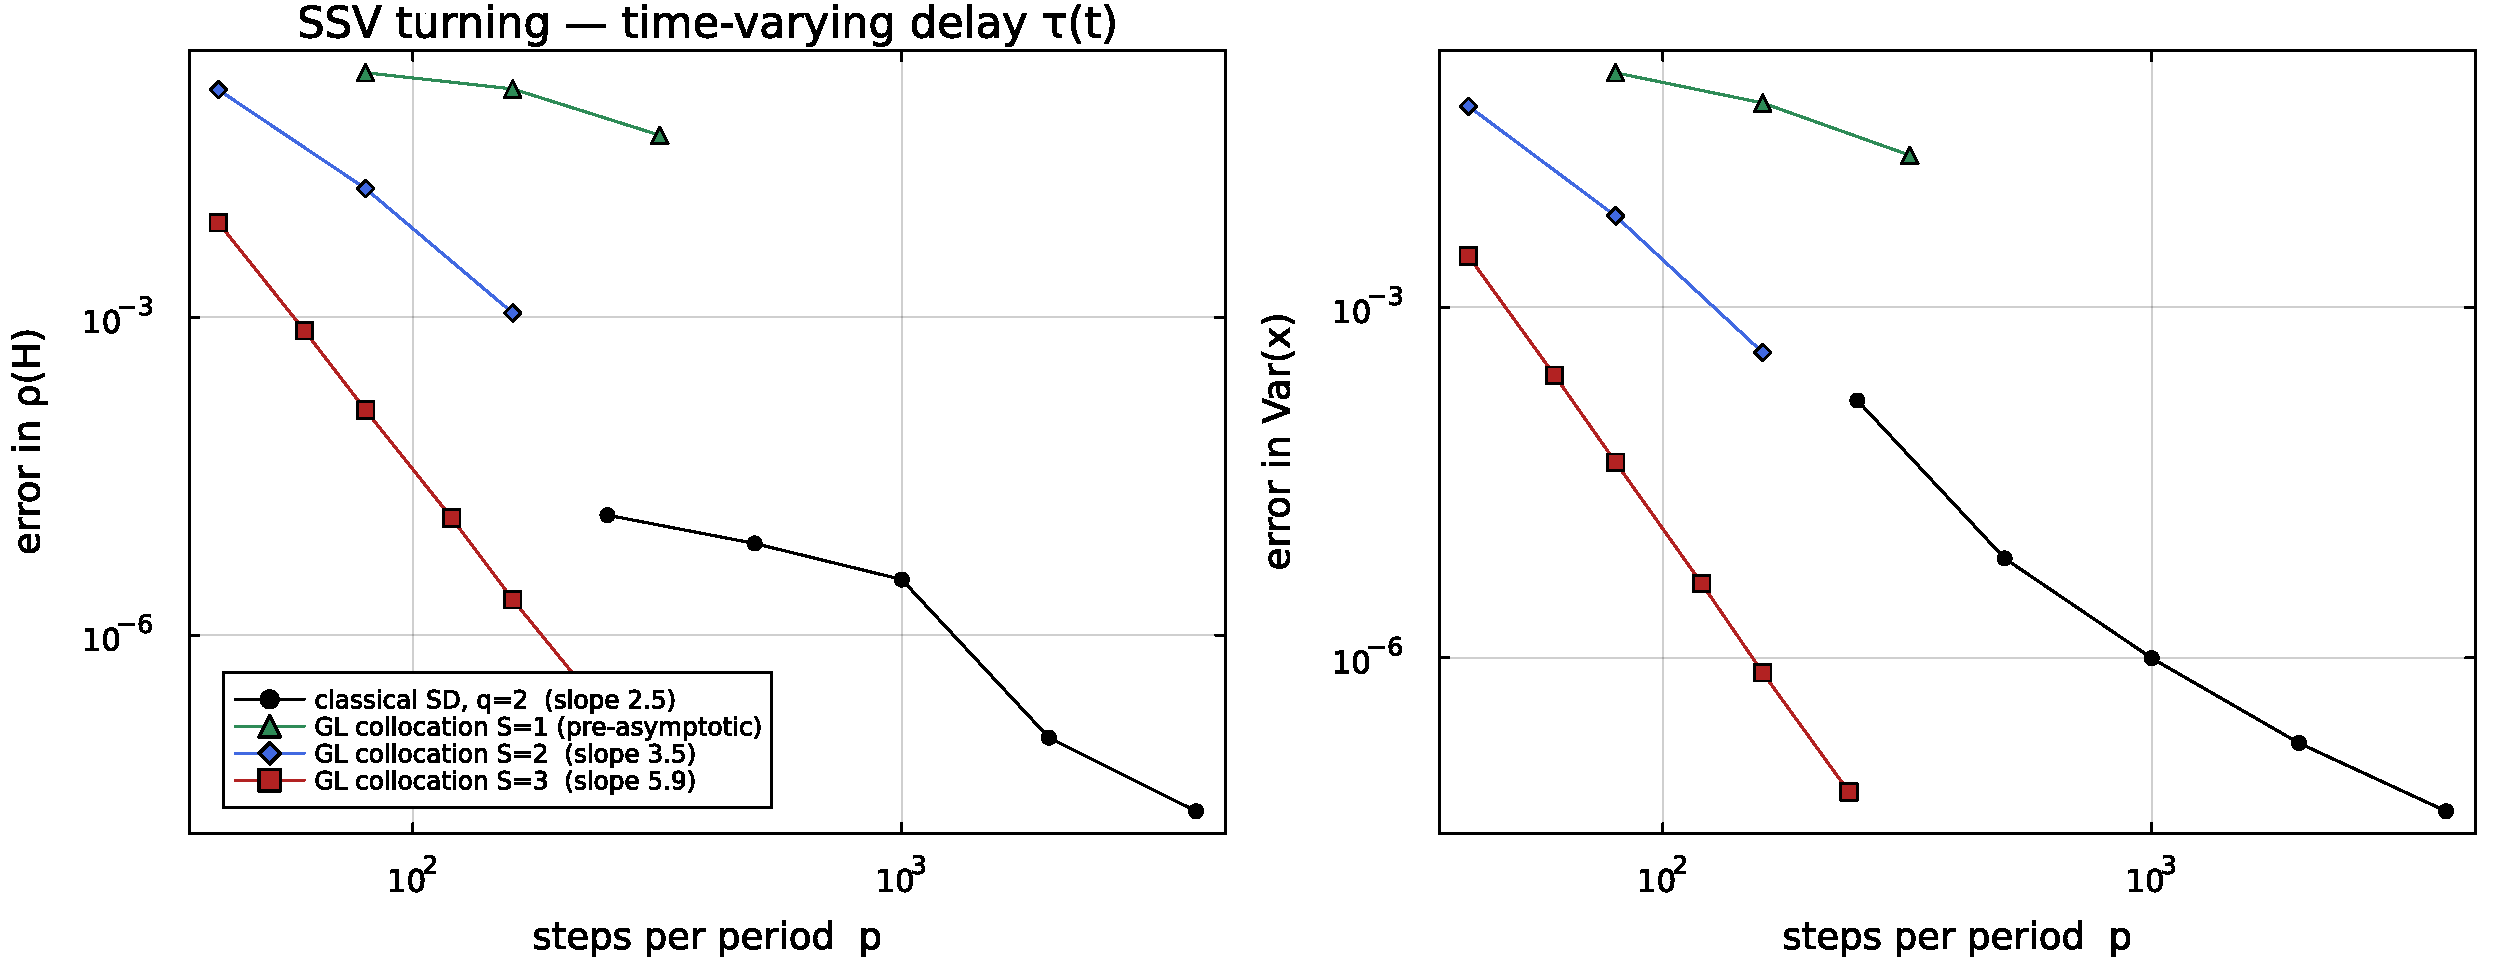
\includegraphics[width=\textwidth]{images/ssv_vt_orders.pdf}
\caption{Second-moment convergence on the SSV turning model with time-varying delay $\tau(t)$: error of the spectral radius $\rho(\mathcal{H})$ (left) and of the stationary variance (right) vs.\ steps per period, for the fractional-limit collocation blocks ($S=1,2,3$, Section~\ref{sec:colloc_tvd}) and the classical scheme ($q=2$). Measured slopes in the legend; $S{=}1$ is pre-asymptotic in this range. On this additive-noise-only problem the classical scheme converges at its deterministic order $\approx 2$ (its generic first-order stochastic cap does not bind), making the comparison conservative.}
\label{fig:ssv_vt}
\end{figure}

\subsection{SSV Milling: Stability Lobes and the Surface-Quality Process Window}
\label{sec:results_ssv}
The final case study exercises every structural feature of the framework at once on the application that motivates it. Spindle speed variation is an established chatter-suppression technique whose stability analysis requires time-periodic coefficients \emph{and} a time-varying regenerative delay \cite{Zatarain2008, Seguy2010, Long2007}. We consider two-DOF milling with full directional cross-coupling between the orthogonal $x$ (feed) and $y$ directions --- a symmetric tool, $\mathbf{q} = [x, y]^\top$ --- with sinusoidal SSV, in the standard dimensionless form (time scaled by the natural angular frequency; cf.\ \cite{Insperger2011, Altintas2012}):
\begin{equation}
\label{eq:milling}
\ddot{\mathbf q} + 2\zeta \dot{\mathbf q} + \mathbf q \;=\; -\,w\, \mathbf{H}(t)\, \big[\mathbf q(t) - \mathbf q(t-\tau(t))\big]\,\big(1 + \sigma_c \dot W_1(t)\big) \;+\; \sigma_a \mathbf{e}_x \dot W_2(t),
\end{equation}
where $w$ is the dimensionless depth of cut (proportional to $a_p K_t$ over the modal stiffness) and $\mathbf{H}(t)$ is the directional cutting-force matrix obtained from the tangential/normal force decomposition (dynamic chip thickness $\Delta x \sin\varphi + \Delta y \cos\varphi$; $F_r = K_r F_t$, $K_r = 0.3$) of a $z=2$-tooth cutter:
\begin{equation}
\label{eq:hfun}
\begin{gathered}
\resizebox{0.9\textwidth}{!}{$\displaystyle
\mathbf{H}(t) = \sum_{j=0}^{z-1} g\big(\varphi_j(t)\big)
\begin{bmatrix}
(\cos\varphi_j + K_r \sin\varphi_j)\sin\varphi_j & (\cos\varphi_j + K_r \sin\varphi_j)\cos\varphi_j \\[2pt]
-(\sin\varphi_j - K_r \cos\varphi_j)\sin\varphi_j & -(\sin\varphi_j - K_r \cos\varphi_j)\cos\varphi_j
\end{bmatrix}$}, \\
\varphi_j(t) = \int_0^t \Omega(s)\,\mathrm{d}s + \tfrac{2\pi j}{z},
\end{gathered}
\end{equation}
with the screen function $g = 1$ while the tooth is in cut and $0$ otherwise. Up-milling is considered with the cut spanning exactly one quarter of the tooth-passing period: $\varphi_{\mathrm{en}} = 0$, $\varphi_{\mathrm{ex}} = \pi/4$ per tooth (the radial immersion $a_D = (1-\cos\varphi_{\mathrm{ex}})/2 \approx 0.146$ follows). The $(1,1)$ entry of $\mathbf{H}$ is the familiar single-DOF directional factor; the off-diagonal entries carry the $x$--$y$ cross-coupling that shapes milling stability in practice. Note that the tooth position $\varphi_j$ advances with the \emph{integral} of the modulated speed, and that the entry/exit discontinuities of $g$ drift relative to the time grid under SSV, so no mesh alignment is possible (or claimed) at these switching instants. The spindle speed is modulated sinusoidally, $\Omega(t) = \Omega_0\big(1 + \mathrm{RVA}\sin(2\pi t/T_{\mathrm{SSV}})\big)$ with $\mathrm{RVA} = 0.25$; the modulation period is $T_{\mathrm{SSV}} = N_{\mathrm{rev}} \cdot 2\pi/\Omega_0$ with $N_{\mathrm{rev}} = 10$ nominal revolutions --- a practically realistic, slow modulation --- and $T_{\mathrm{SSV}}$ is the principal period of the Floquet analysis. For the regenerative delay we use the instantaneous approximation $\tau(t) = (2\pi/z)/\Omega(t)$, which deviates from the exact implicit delay ($\int_{t-\tau}^{t}\Omega\,\mathrm{d}s = 2\pi/z$) at $\mathcal{O}(\mathrm{RVA})$ within one tooth pass --- a standard modeling choice at moderate modulation amplitudes \cite{Long2007, Seguy2010}; the implementation accepts a function-valued delay, discretizes the delayed read with the per-step-averaged delay $\bar\tau_n = \frac{1}{\Delta t}\int_{t_n}^{t_{n+1}}\tau(s)\,\mathrm{d}s$ interpolated to its fractional grid position by the order-$q$ Lagrange stencil, within a buffer sized by $\tau_{\max} = (2\pi/z)/(\Omega_0(1-\mathrm{RVA}))$, and retains the nominal order of the underlying scheme at fixed $\mathrm{RVA}$. The multiplicative noise perturbs the cutting-force coefficient itself ($\sigma_c = 0.2$, at the upper end of the relative force scatter identified in turning experiments \cite{Fodor2020, Fodor2024_PSD}), hence it reads both the present and the delayed tool positions in both directions ($\boldsymbol\beta \ne 0$: the automatic pruning of Section \ref{sec:pruning} correctly stays inactive), and a weak additive source ($\sigma_a = 0.1$, acting in the feed direction) represents broadband force noise; the noise is interpreted in the It\^o sense, and a Stratonovich reading of the physical noise would shift the drift by the correction of Section \ref{sec:theory}, displacing the computed boundaries accordingly. The damping ratio is $\zeta = 0.02$. This stability/quality chart is computed with the classical scheme ($q = 2$); here that is a matter of \emph{correctness}, not merely economy. The interrupted cut makes the directional matrix $\mathbf{H}(t)$ \emph{discontinuous} --- it jumps whenever a tooth crosses the engagement boundary $\varphi_{\mathrm{ex}}$ --- and, as noted above, those switching instants drift across the time grid under SSV. A discontinuity that falls inside a collocation step is spanned by the Gauss--Legendre stage interpolant across the jump, which Gibbs-oscillates: the resulting second-moment spectral radius does not converge under mesh refinement --- we measured it bouncing non-monotonically across the stability threshold as $p$ and $S$ are varied --- so the high-order route cannot place the boundary reliably on this model. The classical scheme, whose step-boundary sampling treats each step piecewise, is robust to the switching and converges cleanly at its first order; it is the appropriate method for an interrupted-cut chart. This limitation is one of \emph{coefficient regularity}, not of the delayed noise or the time-varying delay: the collocation's point-sample $\mathbf{D}_k$ states carry the delayed multiplicative noise ($\boldsymbol\beta \ne 0$) at full order (Section~\ref{sec:colloc_tvd}), and the smooth $\tau(t)$ is handled at high order on the single-axis turning configuration of Section~\ref{sec:results_tvd}. Indeed, the high order is recovered on this very milling model once the engagement is smoothed, as a real helical tool does by averaging the cutting force over the axial depth --- an angular helix-lag window that turns the on/off screen into a continuous engaged fraction. Figure~\ref{fig:helical_order} shows the measured $S=3$ convergence improving with coefficient regularity, from no convergence for the interrupted cut ($C^{-1}$) to order $\approx 3$ for a helical ($C^{0}$) engagement and higher still for a $C^{2}$-smoothed screen, while the classical scheme stays first order throughout.

\begin{figure}[tb]
    \centering
    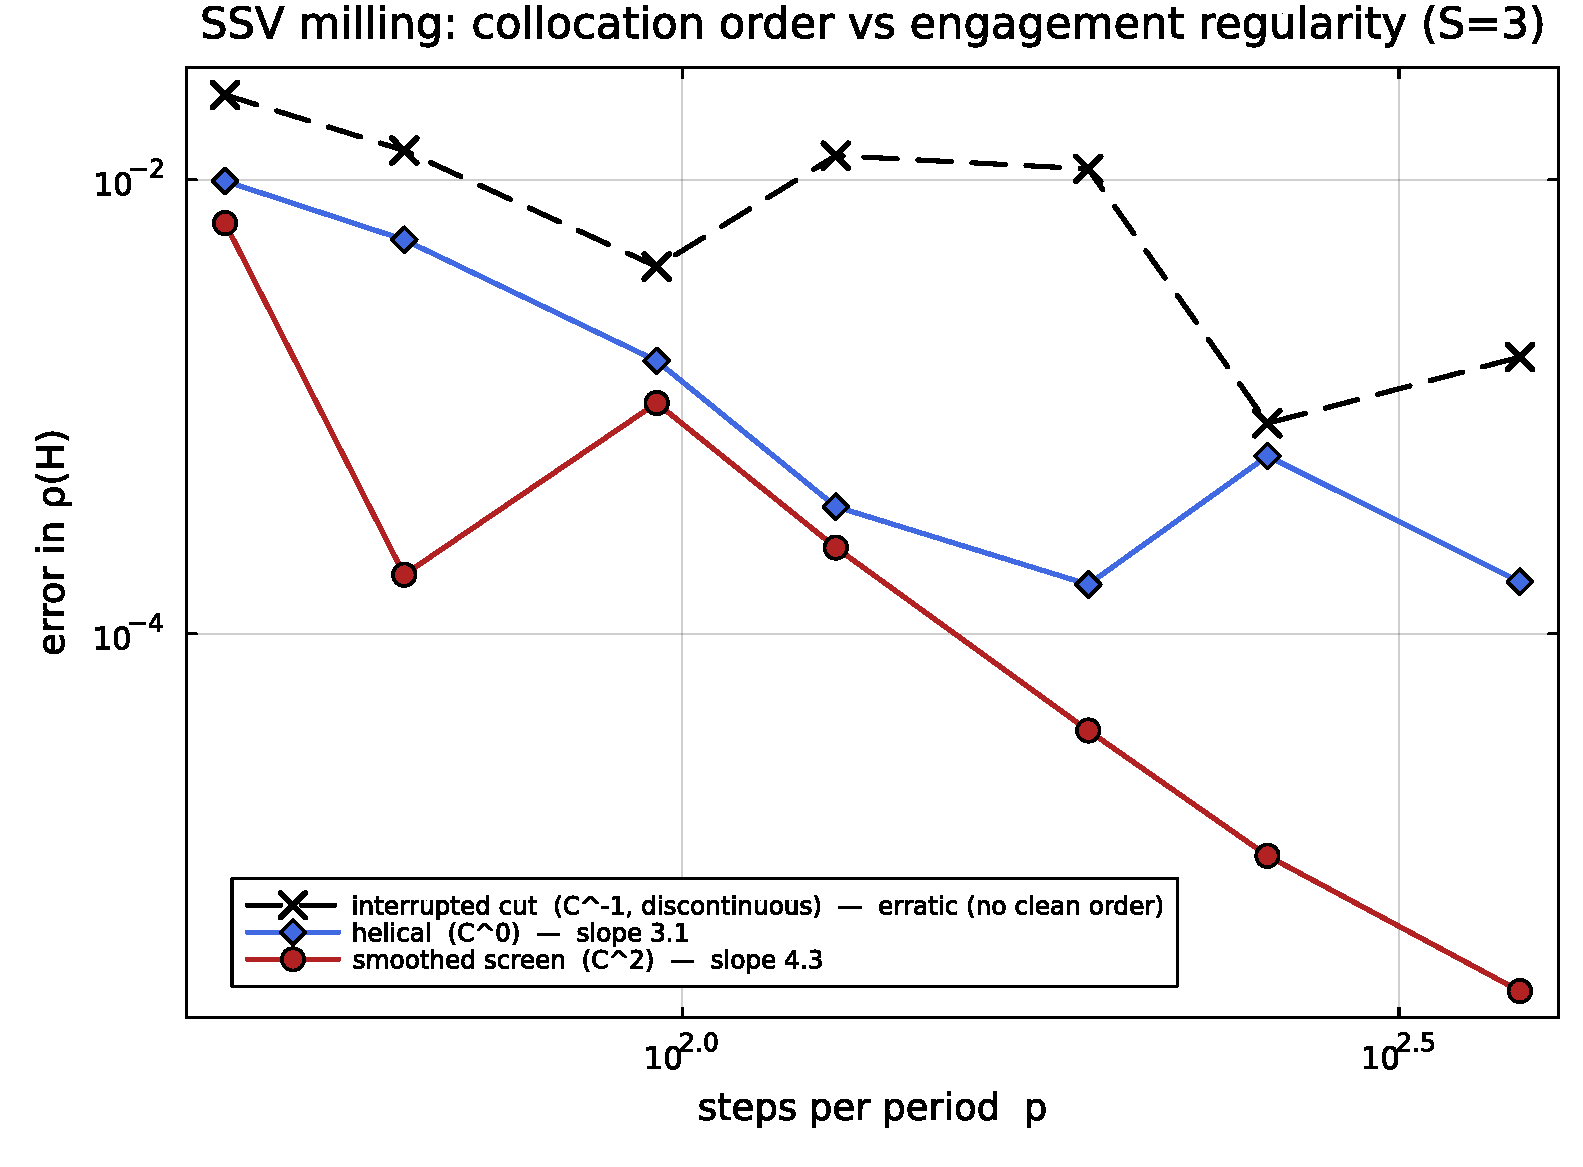
\includegraphics[width=0.72\linewidth]{images/helical_milling_order.pdf}
    \caption{High-order collocation on the SSV \emph{milling} model as a function of the \emph{engagement regularity} (stable operating point $\Omega_0 = 1.0$, $w = 0.25$, stage number $S = 3$): error of the second-moment spectral radius $\rho(\mathcal{H})$ versus steps per principal period $p$. The interrupted straight-tooth cut has a discontinuous ($C^{-1}$) directional matrix and does \emph{not} converge --- its engagement instants drift across the grid and fall inside steps, so the stage interpolant Gibbs-oscillates across the jump (this curve is referenced to the converged classical value; the erratic fine-$p$ behaviour is the point). A helical tool averages the force over the axial depth into a continuous ($C^{0}$) engaged fraction and restores order $\approx 3$; a $C^{2}$-smoothed screen recovers more; the finest points of the convergent curves sit at the accuracy floor of their fine self-references. Reproducible via \texttt{benchmark/helical\_milling\_order.jl}.}
    \label{fig:helical_order}
\end{figure}

\paragraph{Discretization and computational cost.}
The time step resolves both the delay and the structural dynamics, $\Delta t = \min\!\big(\tau_{\max}/24,\; 2\pi/30\big)$ (at least $24$ steps across the longest delay and $30$ steps per natural period), so the number of steps per principal period varies from $360$ for $\Omega_0 \gtrsim 0.83$ (where the delay is the finer scale) to $2400$ at $\Omega_0 = 0.125$ (where $T_{\mathrm{SSV}} = 503$ time units and the natural period sets the step). The variance color map --- a $96\times64$ grid, logarithmically spaced in $\Omega_0$; the $w=0$ row is known in closed form, and every remaining point is a four-dimensional ($d=4$) stochastic moment problem with stationary variance --- completes in $566\,\mathrm{s}$ on $56$ threads of the workstation specified in Section~\ref{sec:results} (Table~\ref{tab:ssv_cost}; the expensive low-$\Omega_0$ columns limit the thread scaling). This configuration is accessible to the multiplication-free evaluation only: at $p = 2400$ steps per period the explicit period product of Eq.~\eqref{eq:period_product} is slower by many orders of magnitude and effectively infeasible (cf.\ Fig.~\ref{fig:wp_ultra}, where it already takes $384\,\mathrm{s}$ and $386\,\mathrm{GB}$ of allocation for a \emph{single} point at $p=192$). As a consistency gate, with the noise switched off the second-moment spectral radius reproduces the squared deterministic Floquet multiplier computed by the independent deterministic semi-discretization package on the same time-varying-delay model class to the discretization accuracy (checked on the single-axis configuration: $2\times10^{-5}$ relative at $r=32$).

The engineering deliverables of Fig.~\ref{fig:ssv} are computed over $\Omega_0 \in [0.125, 1.5]$ (logarithmic speed axis) and $w \in [0, 4]$ with a division of labor that reflects the cost hierarchy of the underlying problems. The variance color map and the two \emph{stochastic} boundaries (the second-moment limit $\rho(\mathcal{H})=1$ and the quality limit $\operatorname{Var}(x)=0.25$) require the factored MF solver of this paper. The two \emph{deterministic} boundaries need only the first-moment monodromy $\rho(\boldsymbol\Phi)$, which the deterministic semi-discretization package \cite{BachrathySDMjl} evaluates through a sparse left/right mapping pair and a matrix-free Krylov eigensolve --- three orders of magnitude cheaper per point, so both deterministic curves are essentially free (Table~\ref{tab:ssv_cost}). All four boundary curves are located by the Multi-Dimensional Bisection Method \cite{Bachrathy2021} on initial grids log-spaced in $\Omega_0$, in a two-phase pattern: a zeroth-order bracketing search over $k$ halving refinements, followed by a single linear-interpolation pass over the final bracketing cubes. After $k$ refinements an $n_1\times n_2$ initial grid resolves the boundary as a uniform grid of $\big((n_1{-}1)2^k{+}1\big)\times\big((n_2{-}1)2^k{+}1\big)$ would, while evaluations are spent only along the boundary --- MDBM pays for boundary \emph{length} where the brute-force map pays for \emph{area}. The deterministic curves at $577\times705$-equivalent resolution resolve fine lobe sub-structure of the modulated system that is invisible at the $96\times64$ resolution of the color map. The practically decisive boundary is the \emph{surface-quality limit} $\operatorname{Var}(x) = 0.25$.

\begin{table}[ht!]
\centering
\small
\caption{Computational cost of the layers of Fig.~\ref{fig:ssv}. Each job ran alone on $56$ threads of the workstation specified in Section~\ref{sec:results}; boundary curves use the two-phase MDBM pattern (zeroth-order bracketing + one linear-interpolation pass). ``Equivalent resolution'' is the uniform grid that a brute-force sweep would need for the same boundary accuracy.}
\label{tab:ssv_cost}
\resizebox{\textwidth}{!}{%
\begin{tabular}{llccrr}
\toprule
layer & solver & initial grid / refinements & equivalent resolution & points & time [s] \\
\midrule
variance color map & MF-SSDM ($\rho$ + fixpoint) & $96\times64$ (full sweep) & $96\times64$ & $6048$ & $566$ \\
(1) const.\ speed, det. & deterministic SD (LR) & $10\times12$ / $6$ & $577\times705$ & $4193$ & $39$ \\
(2) SSV, det.\ $\rho(\boldsymbol\Phi)=1$ & deterministic SD (LR) & $10\times12$ / $6$ & $577\times705$ & $8395$ & $1025$ \\
(3) SSV, $\rho(\mathcal{H})=1$ & MF-SSDM & $10\times6$ / $5$ & $289\times161$ & $846$ & $186$ \\
(4) SSV, $\operatorname{Var}(x)=0.25$ & MF-SSDM (fixpoint) & $10\times6$ / $5$ & $289\times161$ & $629$ & $264$ \\
\bottomrule
\end{tabular}%
}
\end{table} For the zero-mean stationary response of the linear model \eqref{eq:milling} (there is no deterministic forcing here, so the response is purely stochastic; the response is Gaussian in the additive-noise-dominated regime, while strong parametric noise induces excess kurtosis, making the estimate below approximate), the mean absolute deviation of the tool-tip displacement obeys $\mathbb{E}|x| = \sqrt{2/\pi}\,\sigma_x$, and identifying the surface profile height with the tool-tip displacement at the surface-generation instants gives the standard estimate of the \emph{noise-induced contribution} to the arithmetic roughness,
\begin{equation}
\label{eq:ra_formula}
R_a \approx \sqrt{\frac{2}{\pi}} \sqrt{\text{Var}(x)} = \sqrt{\frac{2}{\pi}} \sqrt{\mathbf{M}^*_{x,x}},
\end{equation}
where $\operatorname{Var}(x)$ is evaluated at the period-start phase of the cyclostationary moment. Equation~\eqref{eq:ra_formula} bounds the stochastic contribution only --- deterministic feed marks, runout, and forced vibration contribute additively and are outside the present linear model (cf.\ the surface-location-error literature \cite{HoneycuttSchmitz2017}). In the dimensionless, linear setting the variance scales with $\sigma_a^2$, so the threshold $0.25$ is meaningful relative to the assumed noise intensities; in a physical application the admissible $R_a$ specification, the modal mass, and the length scale of $x$ fix the dimensionless threshold by Eq.~\eqref{eq:ra_formula}.

Regarding physical validity: the deterministic skeleton of Eq.~\eqref{eq:milling} --- the interrupted-cut directional factor and the SSV lobe modification --- belongs to the model class that has been validated against milling experiments in the SSV literature \cite{Zatarain2008, Seguy2010}, and the stochastic layer uses force-noise intensities of the order identified from published cutting-force measurements \cite{Fodor2020, Fodor2024_PSD}; the Monte-Carlo check below verifies the numerics, not the physics, and an experimental validation of the stochastic process map itself remains future work. Figure~\ref{fig:ssv} overlays four boundaries that, read in order, tell the complete story of why the stochastic moment analysis is indispensable for this process. \emph{(1)} The constant-speed process is prone to chatter: its classical deterministic stability lobes (gray dotted) leave only narrow usable pockets. \emph{(2)} Spindle speed variation is applied precisely to overcome this, and the \emph{deterministic} SSV analysis (black dash-dot, $\rho(\boldsymbol\Phi)=1$) indeed predicts a substantially raised admissible depth of cut in the low-speed lobes, in line with the SSV literature \cite{Zatarain2008, Seguy2010}. \emph{(3)} The noise, however, cannot be ignored here: during the modulation cycle the process periodically sweeps through momentarily unstable configurations, and the stochastic excitation is amplified on every pass. The second-moment stability limit $\rho(\mathcal{H})=1$ (blue) therefore lies visibly below the deterministic SSV prediction --- for weaker noise this downward shift of the boundary shrinks, but it does not vanish --- so part of the deterministically ``stable'' gain of SSV is not actually available in a noisy process. \emph{(4)} Even inside the mean-square stable region, stability is not the right criterion: the color map of $\log_{10}\operatorname{Var}(x)$ shows the noise-induced resonance mechanism \cite{Sykora2021_MSSP} at work --- approaching either stability boundary the stationary variance grows by orders of magnitude, and such amplitudes are unacceptable long before the limit is crossed. \emph{Stable does not mean usable}: the vibration-amplitude quality limit $\operatorname{Var}(x)=0.25$ (red dashed) is the boundary that matters, and it lies strictly and non-uniformly below all stability curves. Beyond it the linear model itself loses quantitative validity --- at such amplitudes tool--workpiece contact loss (fly-over) dominates the true dynamics --- so the color map between the quality limit and the stability limit must be read as a qualitative variance-growth indicator only; the nonlinear effects there make the region even less usable than the linear analysis suggests, so the quality boundary is conservative in the safe direction. The engineering conclusion is nuanced: SSV does help --- but by considerably less than the deterministic SSV analysis (itself already nontrivial) predicts, and the actually usable process window can only be identified by the second-moment amplitude analysis introduced in this paper.

As an independent check of the entire chain --- time-varying delay, interrupted-cut coefficients, multiplicative and additive noise --- the stationary variance at the representative stable point $(\Omega_0, w) = (1.0,\, 0.30)$ was validated against a direct Monte-Carlo simulation of Eq.~\eqref{eq:milling}: a semi-implicit (symplectic) Euler--Maruyama ensemble of $2\times10^4$ paths (time step $\Delta t/8$, path-wise time-varying delay with linear history interpolation, $40$ discarded and $20$ averaged modulation periods) yields $\operatorname{Var}(x) = 0.2296 \pm 0.0010$ ($95\%$ confidence), against $0.2267$ from the MF-SSDM fixed point at the chart resolution ($0.2265$ self-converged at sixteenfold resolution) --- an agreement within $1.4\%$, the residual gap being consistent with the $\mathcal{O}(\Delta t)$ weak error of the simulation scheme. We add that this cross-check earns its place in the workflow: it caught a factor-of-two bookkeeping error in the additive-noise accounting of an earlier implementation (an additive source specified on its own Wiener channel was registered once per channel rather than once per source), which the spectral radius --- blind to the additive terms --- could never have revealed; the fixed implementation is guarded by a regression test against the exact limit $\operatorname{Var}(x) = \sigma_a^2/(4\zeta)$ at $w = 0$. We note in passing that a naive \emph{explicit} Euler--Maruyama ensemble is numerically unstable outright at the same time step on this model (the well-known energy drift of the explicit scheme on oscillatory systems turns the mean-square-stable process into a divergent simulation; on the corresponding single-axis model it ``only'' overestimated the variance by $\approx 80\%$), which underlines both the care required in trajectory averaging and the value of a direct moment solver.

\begin{figure}[ht!]
    \centering
    
\includegraphics[width=0.9\textwidth]{images/ssv_chart.png}
    \caption{Stability and surface-quality chart of the two-DOF SSV milling process \eqref{eq:milling} with time-varying delay ($\mathrm{RVA}=0.25$, $T_{\mathrm{SSV}}=10$ revolutions), multiplicative cutting-coefficient noise ($\sigma_c=0.2$) and additive force noise ($\sigma_a=0.1$, feed direction). Color map: $\log_{10}$ of the stationary variance of the feed-direction tool position $x$ over the mean-square stable region; boundary curves located by MDBM \cite{Bachrathy2021}; per-layer computational cost in Table~\ref{tab:ssv_cost}. The four boundaries tell the story in order: (1) gray --- classical deterministic lobes of the \emph{constant-speed} process; (2) black --- deterministic stability limit of the SSV process, $\rho(\boldsymbol\Phi)=1$ (SSV raises the lobes); (3) blue --- second-moment stability limit $\rho(\mathcal{H})=1$ (the noise takes part of that gain back); (4) red --- vibration-amplitude quality limit $\operatorname{Var}(x)=0.25$ (cf.\ Eq.~\eqref{eq:ra_formula}), the practically decisive boundary. The variance diverges toward the stability boundaries (noise-induced resonance), so the usable window is set by the quality limit, not by any stability limit. Between the quality limit and the stability limit the linear model ceases to be quantitatively valid (tool--workpiece contact loss would dominate); the color map there is displayed only to show the variance growth, not as a usable operating region. The three stochastic boundaries are strictly nested --- $\operatorname{Var}=0.25$ (red) inside $\rho(\mathcal{H})=1$ (blue) inside $\rho(\boldsymbol\Phi)=1$ (black) --- as they must be: mean-square stability implies first-moment stability ($\lVert\mathbb{E}\mathbf{x}\rVert^2\le\mathbb{E}\lVert\mathbf{x}\rVert^2$, so $\rho(\mathcal{H})\ge\rho(\boldsymbol\Phi)^2$ pointwise), and a finite stationary variance exists only inside $\rho(\mathcal{H})<1$. At the physical noise level the black and blue boundaries nearly coincide (weak multiplicative noise), so any apparent crossing of the independently traced finite-resolution MDBM curves is a discretization artifact and not a violation of the nesting; amplifying $\sigma_c$ fivefold separates the boundaries visibly and confirms this (supplementary chart, reproducible via \texttt{SSV\_SIGMA\_C=1.0}).}
    \label{fig:ssv}
\end{figure}

\subsection{Cross-validation against a discretization-free formulation}
\label{sec:results_iklodi}
The discretization-free algebraic conditions of Iklodi and Dankowicz \cite{Iklodi2026} provide, on the time-invariant single-delay subclass, an \emph{exact} reference against which the present discretization can be checked --- a stronger benchmark than a Monte-Carlo estimate --- and simultaneously let us quantify the practical cost gap between the two philosophies. Figure~\ref{fig:iklodi} reports both.

\emph{Accuracy.} For their scalar example ($\tau=1$, present multiplicative noise $\alpha=-1.5$, no delayed multiplicative noise), the second-moment stability boundary is available in closed form as the zero set of an elementary-function expression \cite[Eq.~54]{Iklodi2026}. At a point on that boundary the exact second-moment spectral radius equals one, so the quantity $|\rho(\mathcal{H})-1|$ computed by our scheme is pure discretization error. Panel (a) shows this error for the collocation orders $S=1,\dots,5$ at the boundary point $(a,b)=(-3,\,2.6135)$: every scheme converges onto the analytic boundary down to the $\sim\!10^{-11}$ accuracy floor of the iterative eigensolver, reached in under $0.1\,\mathrm{s}$. Two independent routes --- discretization-free algebra and high-order semi-discretization --- thus agree to eleven digits, a machine-precision cross-check of both. On this \emph{scalar, first-order} problem the delayed read $x(t-\tau)$ is only weakly regular (the classical propagation of the initial derivative jump), which limits the asymptotic collocation order to $\approx 4$ irrespective of $S$ --- precisely the rough-delayed-read effect that the integration-by-parts reformulation of Section~\ref{sec:ibp} removes for the delayed-derivative terms of the periodic examples.

\emph{Computational cost.} The final example of \cite{Iklodi2026} is a regenerative \emph{turning} model (their Eqs.~(94)--(95); damping $\zeta=0.05$, force-noise intensity $\sigma=1$) --- a time-invariant, single-delay, two-DOF system carrying present \emph{and} delayed multiplicative noise, squarely within our scope as well. Panel (b) traces its second-moment stability boundary $\rho(\mathcal{H})=1$ with the MF-SSDM (adaptive resolution, $p$ from $24$ at high speed to $\sim\!300$ at the largest delay) located by MDBM \cite{Bachrathy2021}; the reproduced lobe structure and the labelled reference points $A$, $B$, $C$ of \cite[Fig.~13]{Iklodi2026} coincide. The full $774$-point boundary is obtained in $\approx 75\,\mathrm{s}$ on a \emph{single} core of the workstation of Section~\ref{sec:results}. For the same map, \cite{Iklodi2026} reports $22$ hours with a direct pseudo-spectral discretization at their finest resolution ($M=40$; $30$ minutes at $M=20$) and $10$ seconds with their discretization-free continuation. The comparison is instructive: the ``seconds-versus-hours'' advantage of the algebraic method over discretization is, to a large extent, an advantage over a \emph{naive} discretization --- a well-implemented $\mathcal{O}(p^2)$ scheme computes the same boundary in about a minute, within roughly an order of magnitude of the continuation and some three orders of magnitude below the pseudo-spectral cost. Where the discretization-free reduction does not reach --- time-periodic coefficients, and time-varying or multiple delays, which \cite{Iklodi2026} leaves to discretization or to future work --- the multiplication-free semi-discretization remains the practical route, now at a cost that no longer forfeits the comparison.

\begin{figure}[ht!]
    \centering
    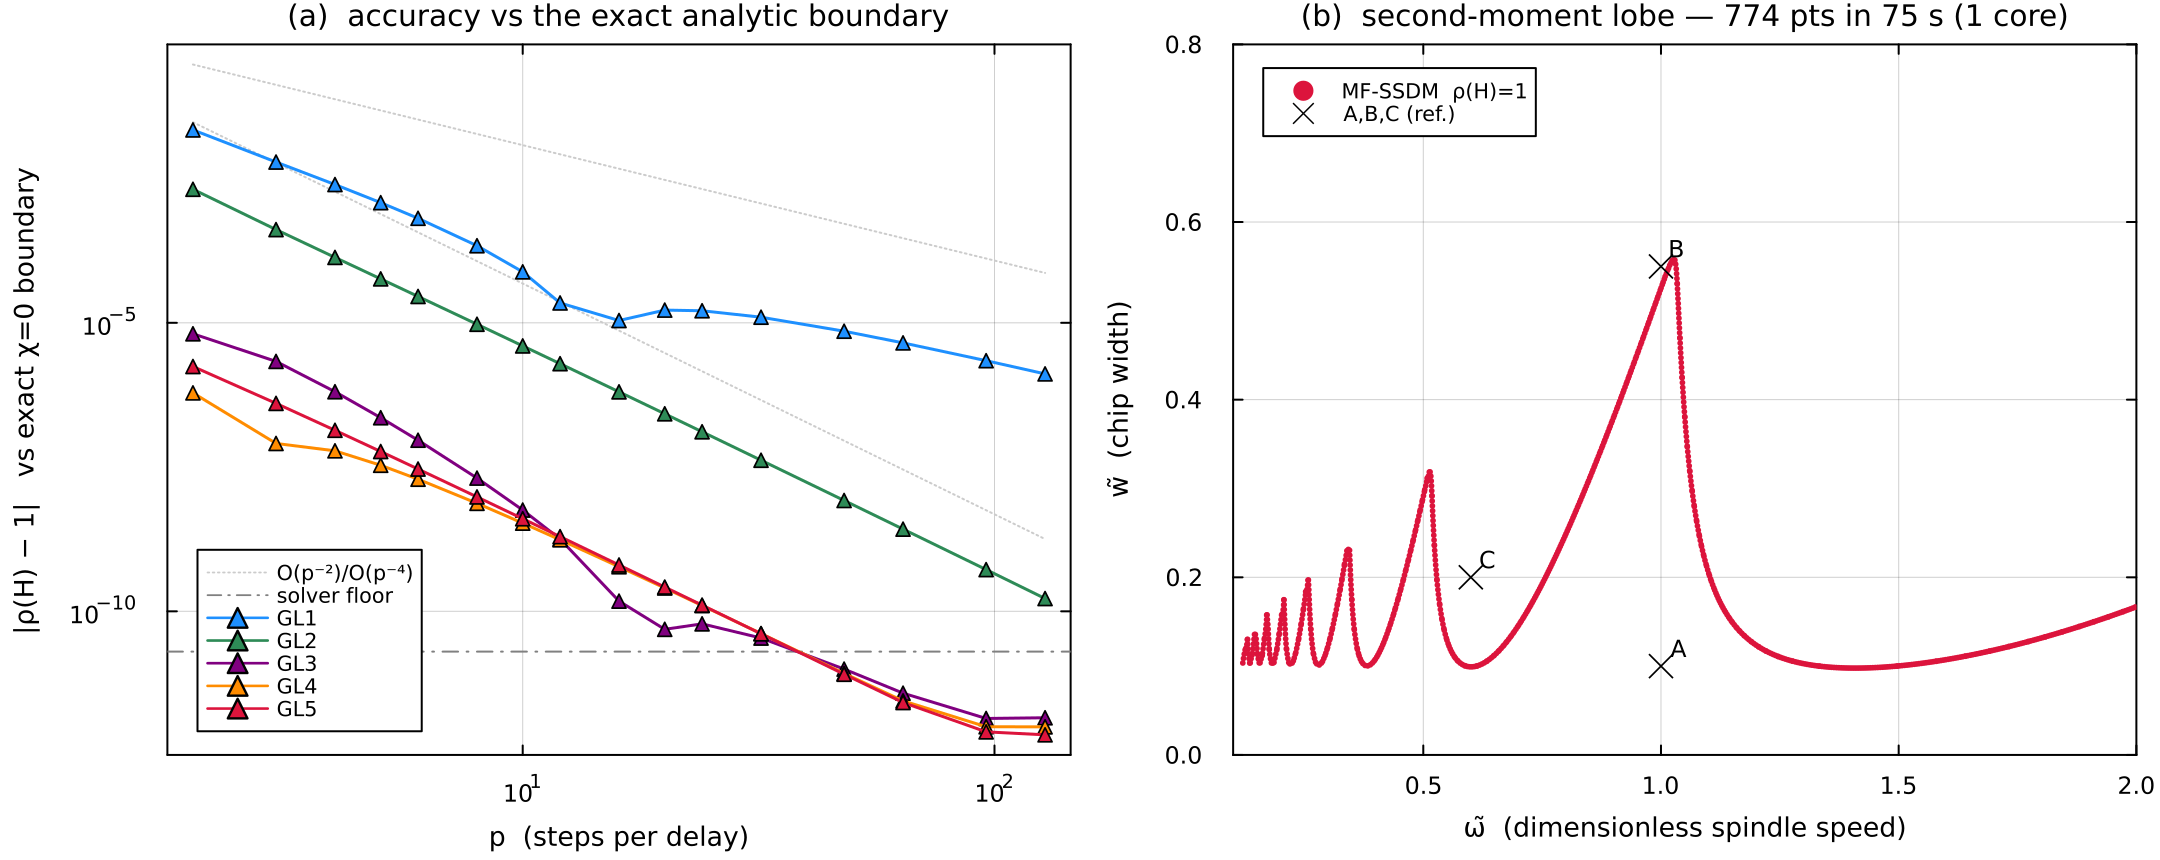
\includegraphics[width=0.95\textwidth]{images/cmp_iklodi.png}
    \caption{Cross-validation against the discretization-free approach of Iklodi and Dankowicz \cite{Iklodi2026}. (a)~Accuracy: error of the collocation second-moment spectral radius against their \emph{exact} scalar boundary $\chi=0$ (\cite[Eq.~54]{Iklodi2026}; $\tau=1$, $\alpha=-1.5$, $\beta=0$) at the boundary point $(a,b)=(-3,2.6135)$, where the true $\rho(\mathcal{H})=1$; all collocation orders reach the $\sim\!10^{-11}$ eigensolver floor, the two independent methods agreeing to eleven digits. (b)~Cost: the second-moment stability lobe $\rho(\mathcal{H})=1$ of their turning benchmark (\cite[Eqs.~(94)--(95), Fig.~13]{Iklodi2026}; $\zeta=0.05$, $\sigma=1$) traced by MF-SSDM${}+{}$MDBM --- $774$ boundary points in $\approx 75\,\mathrm{s}$ on a single core --- reproducing their lobe and reference points $A$, $B$, $C$.}
    \label{fig:iklodi}
\end{figure}

\section{Conclusions and Outlook}
\label{sec:conclusions}

This study addressed a central computational bottleneck of stochastic vibration analysis by introducing the Multiplication-Free Stochastic Semi-Discretization Method (MF-SSDM). The stability analysis of Stochastic Delay Differential Equations (SDDEs) in the semi-discretization framework was previously restricted by the $\mathcal{O}(p^4)$ cost of constructing and multiplying the high-dimensional second-moment step operators. The proposed approach reduces the computational requirement to a strictly quadratic $\mathcal{O}(p^2)$ scaling in execution time, with a correspondingly reduced memory footprint.

The core reformulation decomposes the stochastic transition mapping into a lossless memory shift and a rank-limited boundary injection, evaluated in virtual circular buffers and coupled with Krylov solvers for both spectral stability and stationary moment fixed points; the evaluation is algebraically equivalent to the explicitly assembled discrete operator.

The empirical validations quantify the gain directly. Evaluating the identical discrete operator through the explicit period product and through the multiplication-free recursion, the measured advantage reaches $1.3\times10^3$ in wall-clock time and $6.3\times10^3$ in allocated memory at $p = 192$ (the latter figure refers to cumulative solver allocations; see Section \ref{sec:results}), beyond which the explicit-product route becomes infeasible while the MF route continues to $p = 2048$ and beyond on the same machine. The fractional-limit generalization of the integrated-history blocks removes the constant-delay restriction of the high-order route: on the SSV turning model with genuinely time-varying delay the measured second-moment orders are $3.5$ ($S{=}2$) and $5.9$ ($S{=}3$), at or near the superconvergent $2S$, so the accuracy leap of the collocation blocks now extends to the variable-delay problems that motivate the framework. The SSV milling case study --- a time-varying-delay problem with multiplicative cutting-coefficient noise --- delivers the most important practical result: the surface-quality boundary derived from the stationary variance lies strictly below the second-moment stability boundary across all lobes, so the safe process window is genuinely smaller than any stability analysis alone would indicate.

Beyond the delay-resolution scaling, these extensions broaden the class of tractable problems in orthogonal directions. The Kronecker-factored It\^o operator (Section \ref{sec:kron}) removes the $\mathcal{O}(d^4)$ state-dimension wall of the classical pre-contracted formulation while remaining algebraically identical to it; second-moment stability and stationary variance computations for oscillator chains of one hundred degrees of freedom --- covariance eigenproblems approaching four million unknowns --- complete within minutes on a single workstation, and the factored structure maps naturally onto massively parallel accelerators. The integration-by-parts treatment of rough delayed reads (Section \ref{sec:ibp}) settles a structural question of immediate control-engineering relevance: delayed \emph{proportional} feedback preserves the convergence order of the discretization, whereas the delayed \emph{derivative} term of a PD controller silently collapses it; the exact IBP reformulation restores the order without altering the noise-free consistency of the scheme. Together with the automatic regularity classification of the coefficient matrices, this makes general periodic, delayed, stochastically excited systems under delayed PD control amenable to high-accuracy moment-stability analysis.

The high-order collocation reformulation (Section \ref{sec:colloc}) removes the remaining accuracy barrier of the framework: whereas the classical scheme converges at first order in the second moment for any interpolation order of its deterministic part, the collocation blocks attain a measured order of $2S$ --- rates consistent with order eight at $S=4$, within the resolvable range above the solver floor --- with all structural invariants (noise-free consistency, multiplication-free evaluation, factored contraction) intact. The accompanying work-precision study makes the practical consequence concrete: at engineering tolerances the classical scheme remains an adequate and memory-lean choice, while at tight tolerances the high-order schemes are \emph{more accurate} by three to five orders of magnitude at equal wall-clock time, for the stationary variance exactly as for the spectral radius. The structural pruning of Section \ref{sec:pruning} additionally reduces the memory footprint by a further factor of up to $2.8$ in the common case of delayed feedback control without delayed multiplicative noise, automatically and without user interaction. The two capability extensions must not be conflated: the $(2S+2)^2$ covariance scaling restricts the high-order collocation blocks to low- and moderate-dimensional systems, while high-dimensional problems ($d$ up to hundreds) are covered by the classical-order factored operator; a formulation combining both regimes is an open problem.

Looking forward, a careful It\^o--Taylor treatment of the remaining rough-read residual --- the case where the delayed drift reads a rough component that possesses no smooth antiderivative in the state --- is the subject of ongoing research, as is the port of the factored operator and the collocation blocks to massively parallel accelerators. The longer-term goal is an adaptive-order framework capable of handling state-dependent delays and non-linear stochastic excitations, with applications in model-based process design and monitoring.

\section*{Acknowledgements}
The research leading to these results was supported by the Hungarian National Research, Development and Innovation Office (NKFIH-AG-152125 and NKFIH-PD-146459). H.~T.~Sykora was also supported by the J\'anos Bolyai Research Scholarship of the Hungarian Academy of Sciences (BO/00712/25/6).

\section*{Declaration of competing interest}
The authors declare that they have no known competing financial interests or personal relationships that could have appeared to influence the work reported in this paper.

\section*{CRediT authorship contribution statement}
\textbf{D\'aniel Bachrathy:} Conceptualization, Methodology, Software, Validation, Investigation, Writing -- original draft, Writing -- review \& editing, Supervision. \textbf{Henrik T. Sykora:} Conceptualization, Methodology, Software, Writing -- review \& editing.

\section*{Data availability}
The Julia implementation of all methods of this paper (MF-SSDM, the Kronecker-factored operator, the collocation blocks with automatic pruning, and the GPU path), together with the scripts that generate every figure and table, is openly available in the package \texttt{StochasticSemiDiscretizationMethod.jl} at \url{https://github.com/bachrathyd/StochasticSemiDiscretizationMethod.jl}.

\appendix

\section{The Collocation Block Equations}
\label{app:colloc}

This appendix specifies one step of the Gauss--Legendre collocation covariance update of Section \ref{sec:colloc} explicitly. Let $c_1 < \dots < c_S$ and $a_{ij}, b_j$ denote the nodes and coefficients of the $S$-stage Gauss--Legendre collocation rule on $[0,1]$, $h = \Delta t$ the step, $t_n$ the step start, and $r = \tau/h \in \mathbb{N}$ the delay in steps. Each step stores the block
\begin{equation}
\mathbf{z}_n = \big[\,\mathbf{x}_e;\; \mathbf{Y}_1; \dots; \mathbf{Y}_S;\; \mathbf{J}_1; \dots; \mathbf{J}_S;\; \mathbf{J}_e\,\big] \in \mathbb{R}^{(2S+2)d},
\end{equation}
where $\mathbf{x}_e = \mathbf{x}(t_{n+1})$ is the nodal endpoint, $\mathbf{Y}_i \approx \mathbf{x}(t_n + c_i h)$ are the stage values, and the integrated-history entries are weighted by the delayed-coupling matrix of the step that will read them $r$ steps later,
\begin{equation}
\mathbf{J}_i = \int_0^{c_i h} \mathbf{B}(t_{n+r} + s)\, \mathbf{x}(t_n + s)\, \mathrm{d}s, \qquad i \in \{1,\dots,S\} \cup \{e\},\quad c_e = 1 .
\end{equation}
\paragraph{Deterministic block map.} With $\mathbf{A}_j = \mathbf{A}(t_n + c_j h)$ and the delayed reads supplied \emph{exactly} by the stored integrals of block $n-r$, the stage system and endpoint read
\begin{equation}
\mathbf{Y}_i = \mathbf{x}_n + h \sum_{j=1}^S a_{ij}\, \mathbf{A}_j \mathbf{Y}_j + \mathbf{J}^{(n-r)}_i,
\qquad
\mathbf{x}_e = \mathbf{x}_n + h \sum_{j=1}^S b_j\, \mathbf{A}_j \mathbf{Y}_j + \mathbf{J}^{(n-r)}_e .
\end{equation}
The within-step continuous output $\mathbf{x}(t_n + \theta h) = \mathbf{x}_n + h\sum_j \ell_j(\theta) \dot{\mathbf{Y}}_j$ (with $\ell_j$ the running integrals of the Lagrange basis on the nodes $c_j$ and $\dot{\mathbf{Y}}_j$ the stage derivatives recovered from the $\mathbf{Y}_j$) defines the new integrated-history rows $\mathbf{J}_i$ by Gauss quadrature of $\int_0^{c_i h}\mathbf{B}(t_{n+r}+s)\,\mathbf{x}(t_n+s)\,\mathrm{d}s$; all rows are linear in the window contents, so the step is one block row of a linear map.

\paragraph{Within-step noise covariance.} Let $\boldsymbol\eta(u)$ denote the noise-driven state perturbation accumulated inside the current step ($\boldsymbol\eta \equiv \mathbf{0}$ at all window nodes; delayed reads of $\boldsymbol\eta$ vanish because $\tau \ge h$). Its equal-time covariance $\boldsymbol\Sigma_\eta(u) = \mathbb{E}[\boldsymbol\eta(u)\boldsymbol\eta(u)^\top]$ obeys the within-step Lyapunov equation
\begin{equation}
\begin{split}
\boldsymbol\Sigma_\eta' = {}& \mathbf{A}\boldsymbol\Sigma_\eta + \boldsymbol\Sigma_\eta \mathbf{A}^\top \\
&+ \sum_k \Big[\boldsymbol\alpha_k \mathbf{P}_{xx} \boldsymbol\alpha_k^\top + \boldsymbol\alpha_k \mathbf{P}_{x\tau} \boldsymbol\beta_k^\top + \boldsymbol\beta_k \mathbf{P}_{x\tau}^\top \boldsymbol\alpha_k^\top + \boldsymbol\beta_k \mathbf{P}_{\tau\tau} \boldsymbol\beta_k^\top + \hat{\boldsymbol\gamma}_k\hat{\boldsymbol\gamma}_k^\top\Big](u),
\end{split}
\end{equation}
where $\mathbf{P}_{xx}, \mathbf{P}_{x\tau}, \mathbf{P}_{\tau\tau}$ denote the present/delayed covariance blocks of the current window read at the stage nodes, and $\hat{\boldsymbol\gamma}_k$ the additive loading; the equation is solved by the same collocation rule. (The $\mathcal{O}(\Delta t)$ feedback of $\boldsymbol\Sigma_\eta$ itself onto the multiplicative injection is neglected, consistent with the collocation order.) For the \emph{two-time} entries the drift-propagation identity of linear It\^o systems applies: for $u \le v$,
\begin{equation}
\label{eq:causal_kernel}
\begin{gathered}
\mathbb{E}\big[\boldsymbol\eta(u)\,\boldsymbol\eta(v)^\top\big] \;=\; \boldsymbol\Sigma_\eta(u)\, \boldsymbol\Psi(v,u)^\top, \\
\boldsymbol\Psi(v,u) = \text{present-drift propagator from } u \text{ to } v,
\end{gathered}
\end{equation}
because the martingale increments on $(u,v]$ are uncorrelated with $\boldsymbol\eta(u)$ and the delayed argument of $\boldsymbol\eta$ vanishes within the step. Equation \eqref{eq:causal_kernel} is exact for the locally frozen (within-step collocation) dynamics; its use constitutes an approximation only at the collocation order of the step itself. All node--node, node--integral ($\int \mathbf{B}\,\boldsymbol\eta$), and integral--integral covariance entries of the new block are Gauss quadratures of \eqref{eq:causal_kernel} over the corresponding (triangle-split) domains. The per-step noise injection assembled this way is what Section \ref{sec:colloc} refers to as the kernel fill; the measured order $2S$ of the composed scheme is empirical, consistent with the collocation order of every ingredient above, and no formal proof is claimed. The reference implementation of this appendix is contained in the accompanying package (see the Data Availability statement).

\section{Zeroth-Order Coefficient Blocks}
\label{app:blocks}
For completeness, the explicit zeroth-order deterministic blocks referenced in Section \ref{sec:theory}, with $\mathbf{A}_{\mathrm{avg}} = \frac{1}{\Delta t}\int_{t_n}^{t_{n+1}}\mathbf{A}(s)\,\mathrm{d}s$:
\begin{equation}
\mathbf{F}_{n,0} = \exp(\mathbf{A}_{\mathrm{avg}} \Delta t), \qquad
\mathbf{F}_{n,r} = \left(\int_0^{\Delta t} \exp(\mathbf{A}_{\mathrm{avg}}(\Delta t - s))\, \mathrm{d}s\right) \mathbf{B}(t_n);
\end{equation}
the higher-order ($q \ge 1$) interpolated variants follow \cite{Insperger2011, Sykora2019} and are implemented in the accompanying package.

\section{GPU Implementation and Dimensional Scaling}
\label{app:gpu}

The multiplication-free recursion is a sequence of many small, mutually independent block operations --- a structure that maps naturally onto massively parallel hardware, but only if the classical GPU pitfall is avoided: if every Krylov iteration ships the covariance between host and device, the transfer time dominates and the accelerator idles. Our implementation therefore keeps the \emph{entire} computation resident on the device: the coefficient samples are uploaded once, the full $p$-step covariance recursion and the complete Krylov iteration execute on the GPU (using cooperative kernels with a single grid-wide synchronization per step, and a load-balanced variant of the diagonal It\^o contraction for larger $d$), and only the converged Floquet multiplier is returned to the host. In the accompanying Julia package this is a one-line switch: \texttt{spectralRadiusOfMapping\_GPU} replaces \texttt{spectralRadiusOfMapping\_MF} (an automatic variant selects the GPU whenever a functional CUDA device is present); no other user code changes. The device-memory budget is stated explicitly, since it is the hard wall of the approach: the resident data comprise the Krylov basis, $(k_{\mathrm{dim}}{+}2)$ vectors of the $\operatorname{vech}$ dimension $D = \tfrac12 W(W{+}1)$, $W = d(r{+}1)$, i.e.\ $\mathrm{VRAM} \approx 8\,(k_{\mathrm{dim}}{+}2)\,D$ bytes plus the $\mathcal{O}(K d^2 p)$ coefficient samples. With $k_{\mathrm{dim}} = 15$ this is $4.6\,\mathrm{GB}$ at $d=2$, $p=4096$ and $0.12\,\mathrm{GB}$ at $d=10$, $p=256$ --- all experiments reported here fit the 8-GB workstation card --- while e.g.\ $d = 20$, $p = 1024$ ($D \approx 2.1\times10^8$) would demand $\approx 28\,\mathrm{GB}$ and $d=200$, $p=256$ is beyond any current accelerator. Larger problems require either a smaller Krylov dimension, restarted iterations trading time for memory, or multi-GPU partitioning; none of these is claimed here.

Figure \ref{fig:gpu_chain} reports measured wall-clock times for periodic, delayed, stochastically excited oscillator chains of $1$--$5$ degrees of freedom ($d = 2$--$10$ state variables) over resolutions $p = 16$--$256$, on a workstation GPU (NVIDIA Quadro P4000, whose FP64 throughput is $1/32$ of its FP32 rate). The CPU and GPU paths agree in the spectral radius to $5\times10^{-13}$ over the whole dataset (and to $1.5\times10^{-14}$ on the fully periodic Mathieu benchmark up to $p=4096$). At small $p$ and small $d$ the GPU is slower --- kernel-launch latency dominates and the device is under-occupied ($d=2$ reaches break-even only near $p \approx 200$, $d=4$ near $p \approx 90$) --- while the speedup grows with both the resolution and the state dimension, reaching $5$--$6\times$ at $d = 10$, $p = 256$, because larger blocks saturate the device occupancy. On accelerators with full-rate FP64 the crossover is expected to shift substantially further in favor of the GPU, given the $32\times$ FP64 handicap of the present workstation card; this remains to be measured. The GPU path currently covers the classical-order MF-SSDM operator; a GPU port of the collocation blocks of Section \ref{sec:colloc} is planned.

\begin{figure}[ht!]
    \centering
    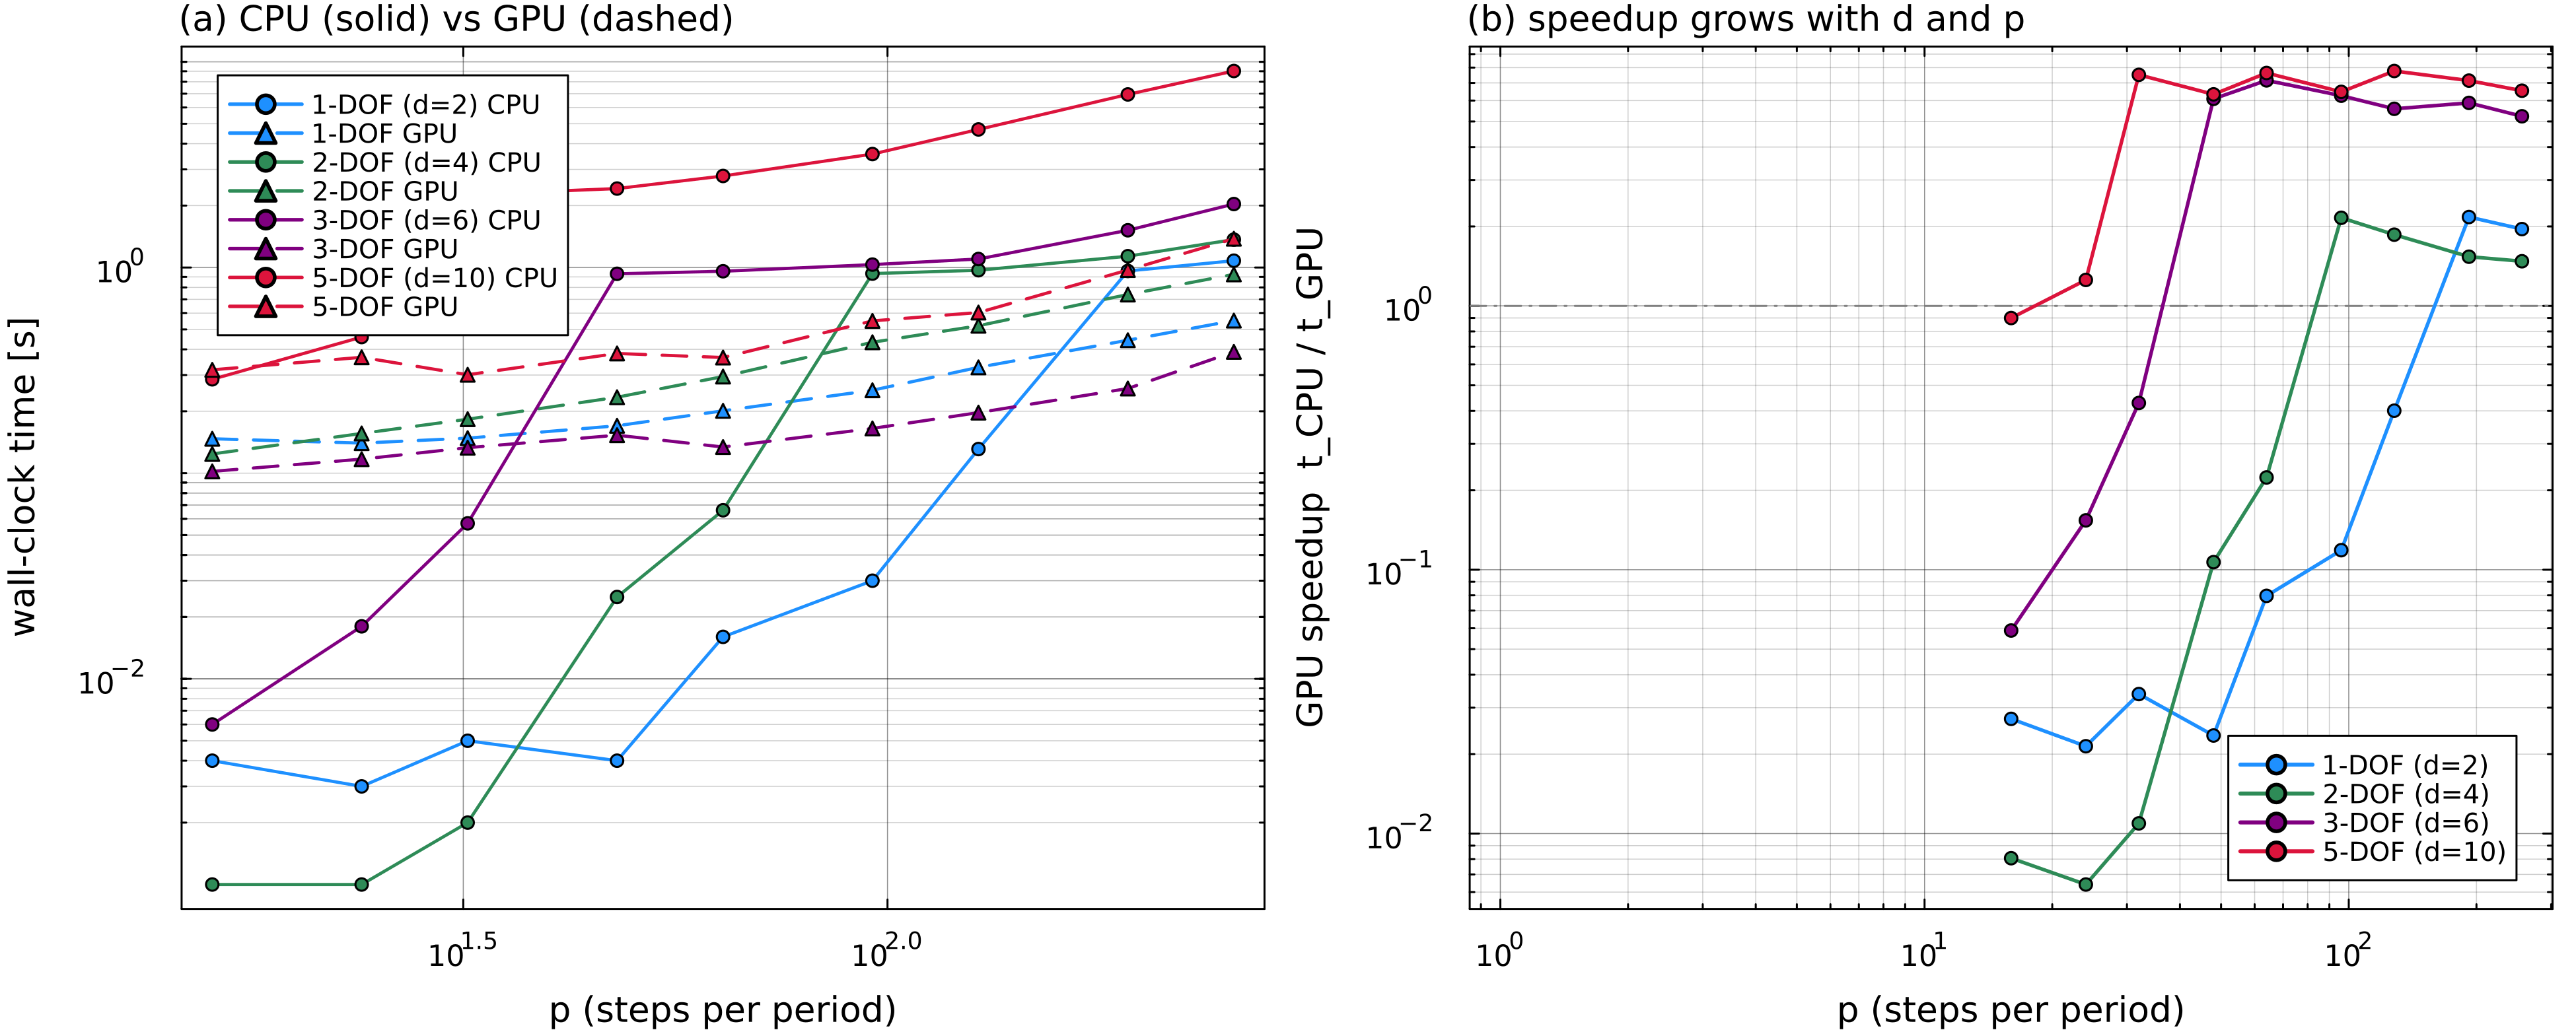
\includegraphics[width=0.95\textwidth]{images/gpu_chain_scaling.png}
    \caption{GPU scaling of the MF-SSDM spectral-radius solve for oscillator chains of increasing dimension (all coefficients time-periodic, present and delayed multiplicative noise). (a) Wall-clock time, CPU (solid) vs GPU (dashed); (b) GPU speedup. Spectral radii agree to $5\times10^{-13}$ between the two paths. NVIDIA Quadro P4000; the entire Krylov iteration runs on the device, only the Floquet multiplier is transferred back.}
    \label{fig:gpu_chain}
\end{figure}

\section{Dimensional Reach: Parametrically Excited FE Beam with Delayed PD Control}
\label{app:beam}

To demonstrate the dimensional reach of the Kronecker-factored operator on a physically motivated model, we consider a pinned--pinned Euler--Bernoulli beam under a pulsating axial load $P(t) = P_0 + P_1 \cos \Omega t$ (parametric excitation) with an active damper applying a delayed PD force at a sensor/actuator location $x_s$, and multiplicative noise on the axial load. A standard finite-element discretization with $n_e$ elements yields
\begin{equation}
\label{eq:beam}
\mathbf{M}\ddot{\mathbf q} + \mathbf{C}\dot{\mathbf q} + \big[\mathbf{K} - P(t)\, \mathbf{G}\big] \mathbf q
= \mathbf{b}_s \big[ k_P\, q_s(t-\tau) + k_D\, \dot q_s(t-\tau) \big]
+ \text{noise},
\end{equation}
where $\mathbf{G}$ is the geometric stiffness matrix and $q_s = \mathbf{b}_s^\top \mathbf{q}$ (in this appendix $\mathbf{M}, \mathbf{C}, \mathbf{K}, \mathbf{G}$ denote the structural matrices, not the global covariance symbols of the main text). The single-mode Galerkin reduction of Eq.~\eqref{eq:beam} is precisely the PD-controlled Mathieu oscillator \eqref{eq:pd_mathieu}, so this example continues the benchmark thread at increasing fidelity. The engineering question is modal convergence: how many modes of the (fine, $n_e=128$) finite-element model must be retained before the second-moment spectral radius $\rho(\mathcal{H})$ is trustworthy, and whether the converged, high-dimensional computation is affordable.

All quantities are dimensionless with $EI = \rho A = L = 1$, so the pinned--pinned natural frequencies are $\omega_i = (i\pi)^2$; cubic Hermite elements are used, and the modal basis is $\mathbf{M}$-normalized. The full parameter set is: axial load $P_0 = 3.0$, $P_1 = 4.0$, excitation at the third-mode parametric resonance $\Omega = 2\omega_3 = 2(3\pi)^2$, delay $\tau = 2\pi/\Omega$ (equal to the principal period), sensor/actuator location $x_s = 0.37$ with $\mathbf{b}_s$ the Hermite shape-function evaluation at $x_s$, delayed gains $k_P = k_D = 3.0$, modal damping $\mathbf{C}_r = \operatorname{diag}(2\zeta_1\omega_i)$ with $\zeta_1 = 0.002$, and multiplicative noise on the axial load: the ``noise'' term of Eq.~\eqref{eq:beam} is $-\sigma_P\,\mathbf{G}\,\mathbf{q}\;\dot W(t)$ with $\sigma_P = 1.5$ (the stochastic part of $P(t)$ reads the positions through the geometric stiffness). We project the $n_e = 128$ model onto its lowest $n_m$ modes and evaluate $\rho(\mathcal{H})$ at fixed discretization ($p = 64$, $q = 0$, It\^o quadrature $K = 20$) for $n_m = 1,\dots,16$. Two consistency gates precede the sweep: the factored and dense second-moment operators agree to $3\times10^{-16}$ on a common test vector, and with the noise switched off $\rho(\mathcal{H})$ reproduces $\rho(\boldsymbol{\Phi})^2$ of the deterministic monodromy operator to $4\times10^{-15}$.

Figure \ref{fig:beam_mesh} shows the result. The spectral radius converges monotonically from $\rho = 1.2214$ (single-mode model, the Mathieu-oscillator fidelity) to $\rho = 1.22545$; the single-mode model underestimates the growth rate by $4\times10^{-3}$, and mode-truncation errors decay roughly geometrically: the relative truncation error drops below $10^{-4}$ for $n_m \ge 4$ and below $3\times10^{-6}$ for $n_m \ge 12$. The largest computation, $n_m = 16$ ($d = 32$ state variables), corresponds to a covariance fixed-point problem with $D = 2.16\times10^{6}$ unknowns and completes in $142\,\mathrm{s}$ on a workstation CPU with the Kronecker-factored operator --- a problem size at which the dense coefficient tensor ($\mathcal{O}(p^2 d^4)$ storage) could not even be assembled (cf.\ Table \ref{tab:kron_scaling}).

\begin{figure}[ht!]
    \centering
    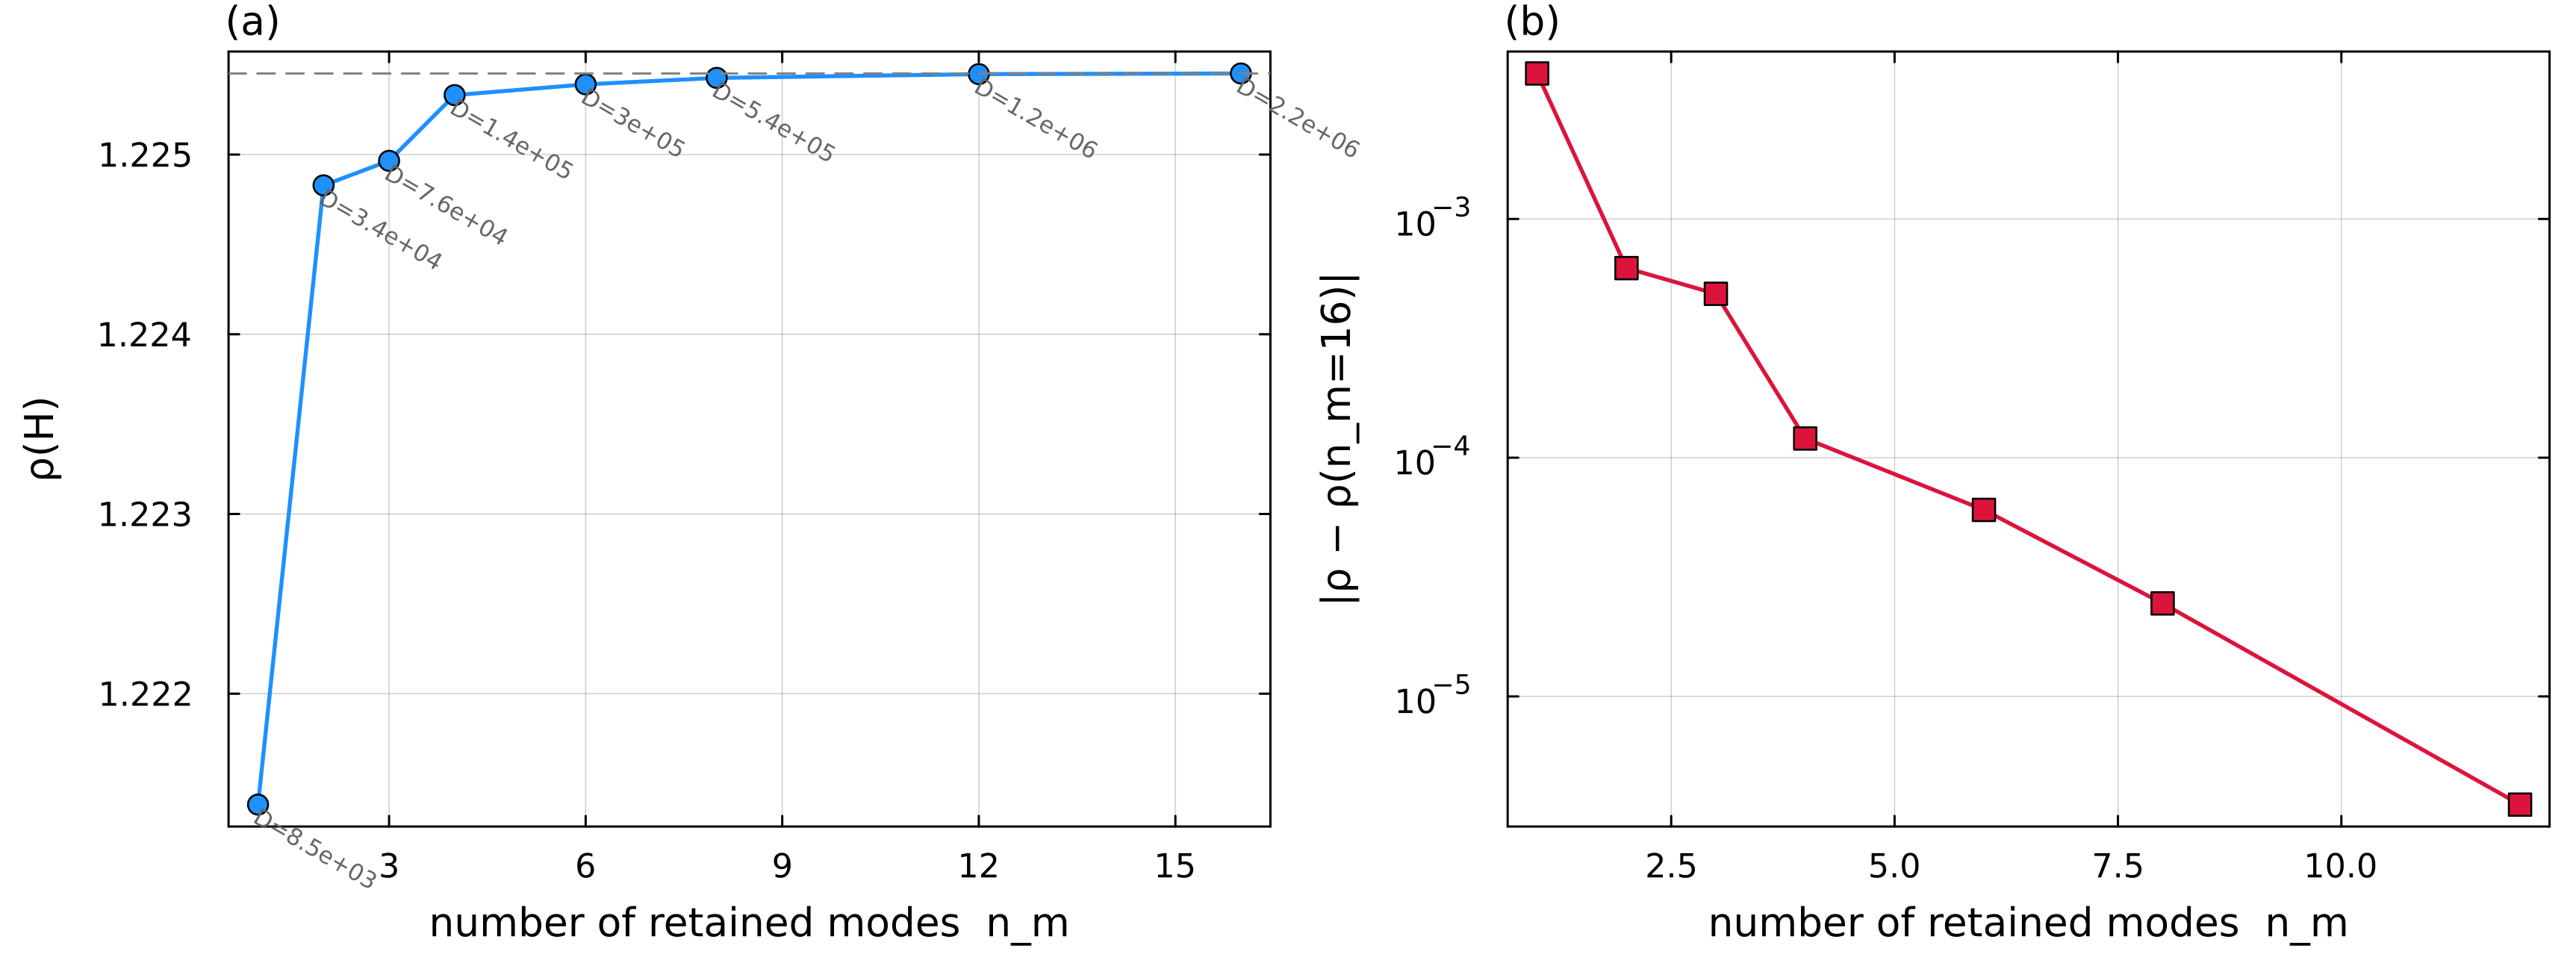
\includegraphics[width=0.9\textwidth]{images/beam_mesh_convergence.png}
    \caption{Modal convergence of the second-moment spectral radius for the actively controlled, parametrically excited beam \eqref{eq:beam} at $\Omega \approx 2\omega_3$ ($n_e = 128$ finite elements, $p=64$). (a) $\rho(\mathcal{H})$ vs the number of retained modes $n_m$, annotated with the covariance problem size $D$; (b) mode-truncation error relative to the $n_m=16$ model. The Kronecker-factored operator makes the converged computation ($D = 2.16\times10^{6}$ unknowns, $142$~s) routine.}
    \label{fig:beam_mesh}
\end{figure}

\bibliographystyle{elsarticle-num}
\bibliography{references}

\end{document}
